%%%%%%%%%%%%%%%%%%%%%%%%%%%%%%%%%%%%%%%%%
%  My documentation report
%  Objetive: Explain what I did and how, so someone can continue with the investigation
%
% Important note:
% Chapter heading images should have a 2:1 width:height ratio,
% e.g. 920px width and 460px height.
%
%%%%%%%%%%%%%%%%%%%%%%%%%%%%%%%%%%%%%%%%%

%----------------------------------------------------------------------------------------
%	PACKAGES AND OTHER DOCUMENT CONFIGURATIONS
%----------------------------------------------------------------------------------------

\documentclass[12pt,fleqn]{book} % Default font size and left-justified equations

%\usepackage[top=3cm,bottom=3cm,left=3.2cm,right=3.2cm,headsep=10pt,letterpaper]{geometry} % Page margins
\usepackage[left=2cm,right=2cm, top=2cm,bottom=2cm,headsep=12pt,letterpaper]{geometry} % Page margins


\usepackage{xcolor} % Required for specifying colors by name
\definecolor{ocre}{RGB}{52,177,201} % Define the orange color used for highlighting throughout the book

% Font Settings
\usepackage{avant} % Use the Avantgarde font for headings
%\usepackage{times} % Use the Times font for headings
\usepackage{mathptmx} % Use the Adobe Times Roman as the default text font together with math symbols from the Sym­bol, Chancery and Com­puter Modern fonts

\usepackage{enumerate}
\usepackage{multicol}
\usepackage{multirow}
\usepackage{caption}
\usepackage{microtype} % Slightly tweak font spacing for aesthetics
\usepackage[utf8]{inputenc} % Required for including letters with accents
\usepackage[T1]{fontenc} % Use 8-bit encoding that has 256 glyphs

% Bibliography
%\usepackage[style=alphabetic,sorting=nyt,sortcites=true,autopunct=true,babel=hyphen,hyperref=true,abbreviate=false,backref=true,backend=biber]{biblatex}
%\addbibresource{bibliography.bib} % BibTeX bibliography file
%\defbibheading{bibempty}{}

\input{structure} % Insert the commands.tex file which contains the majority of the structure behind the template

\begin{document}

%----------------------------------------------------------------------------------------
%	TITLE PAGE
%----------------------------------------------------------------------------------------

\newcommand{\institutionauthor}{Personal Teaching}
\begingroup
\thispagestyle{empty}
\AddToShipoutPicture*{\put(0,0){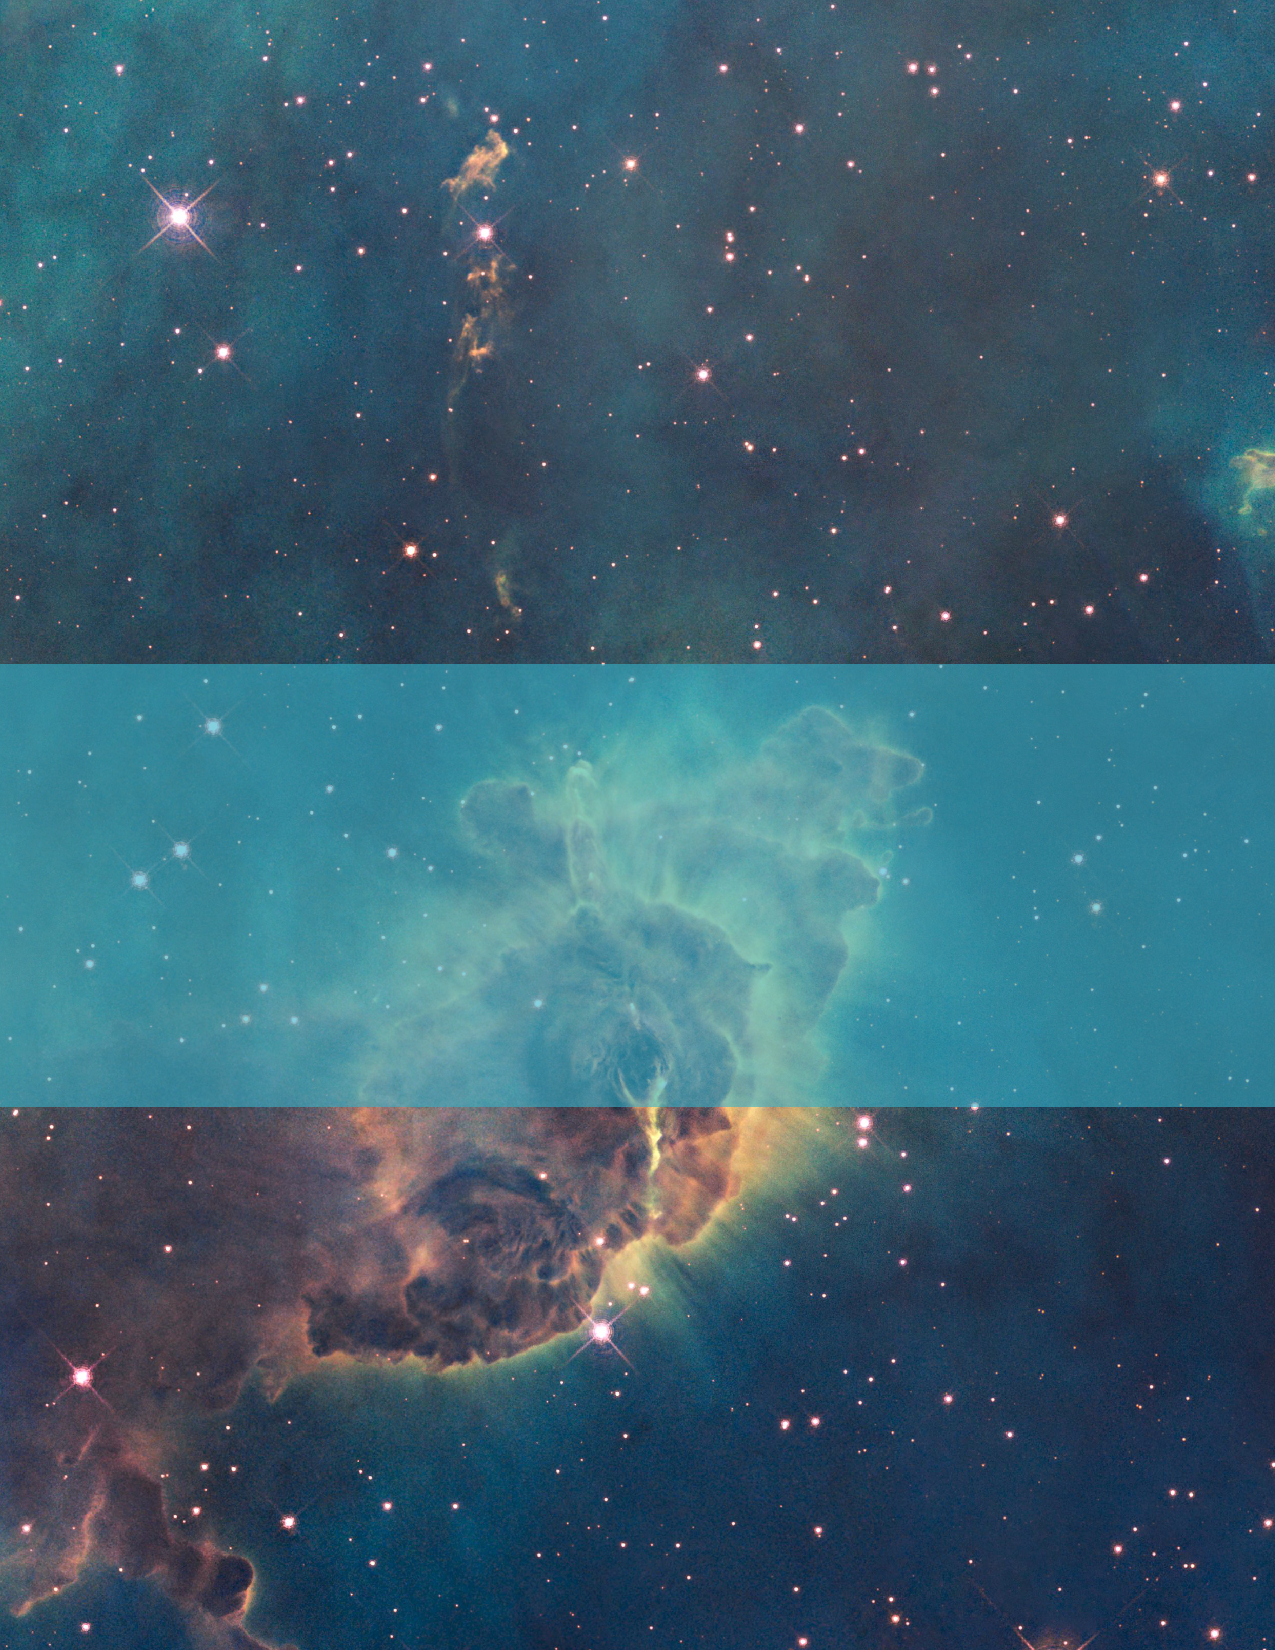
\includegraphics[scale=1.25]{esahubble}}} % Image background
\centering
\vspace*{5.8cm}
\par\normalfont\fontsize{35}{35}\sffamily\selectfont
\textbf{Cartilla Pre ICFES}\\
\vspace*{0.5cm}
{\Huge Personal Teaching}\par % Book title
{\Huge 2015}\par % Book title
\vspace*{1.cm}
{\LARGE Editor J. S. Castellanos-Durán}\par
%{\LARGE 2015}\par % Author name
\endgroup

%----------------------------------------------------------------------------------------
%	COPYRIGHT PAGE
%----------------------------------------------------------------------------------------

\newpage
~\vfill
\thispagestyle{empty}

%\noindent Copyright \copyright\ 2014 Andrea Hidalgo\\ % Copyright notice

\noindent \textsc{\copyright Personal Teaching}\\

\noindent \textit{Marzo 2015} % Printing/edition date



%%%%%%%%%%%%%%%%%%%%%%%%%%%%%%%%%%%%%%%%%%%%%%%%%%
%%%%%%%%%%%%  Cabezote    %%%%%%%%%%%%%%
%%%%%%%%%%%%%%%%%%%%%%%%%%%%%%%%%%%%%%%%%%%%%%%%%%

%\newpage
\vfill
\begin{center}
\begin{Huge}
Caratula
\end{Huge}

\vfill
Bogotá D.C. 2014

\end{center}
\vfill

%%%%%%%%%%%%%%%%%%%%%%%%%%%%%%%%%%%%%%%%%%%%%%%%%%

\newpage
\vfill
\begin{center}
\begin{Huge}
Ficha técnica
\end{Huge}
\vfill
\par
\textbf{Gerente general}\\
...\\
\textbf{Profesores}\\
...
\par

\vfill
Bogotá D.C. 2014

\end{center}
\vfill

%%%%%%%%%%%%%%%%%%%%%%%%%%%%%%%%%%%%%%%%%%%%%%%%%%

\newpage
\vfill
\begin{center}
\begin{Huge}
Prefacio
\end{Huge}
\vfill
\par

En esta cartilla ... gracias a ... dedicada a...
\par

\vfill
Bogotá D.C. 2014

\end{center}
\vfill


%----------------------------------------------------------------------------------------
%	TABLE OF CONTENTS
%----------------------------------------------------------------------------------------

\chapterimage{head1.png} % Table of contents heading image

\pagestyle{empty} % No headers

\tableofcontents % Print the table of contents itself

%\cleardoublepage % Forces the first chapter to start on an odd page so it's on the right

\pagestyle{fancy} % Print headers again


%----------------------------------------------------------------------------------------
%	CHAPTER 1
%----------------------------------------------------------------------------------------

\chapterimage{blanck.jpg} % Chapter heading image

\chapter{Introducción}


\twocolumn

%%%%%%%%%%%%%%%%%%%%%%%%%%%%%%%%%%%%%%%%%%%%%%%%%%
%%%%%%%%%%%%   Ciencias Mathematics %%%%%%%%%%%%
%%%%%%%%%%%%%%%%%%%%%%%%%%%%%%%%%%%%%%%%%%%%%%%%%%
\newpage

\chapterimage{math3v.jpg} % Table of contents heading image

\chapter{Matemáticas I}\label{chap:math1}

\subsubsection*{Responda las preguntas \ref{vic-1} y \ref{vic-2} con base en la siguiente informaci\'on.}

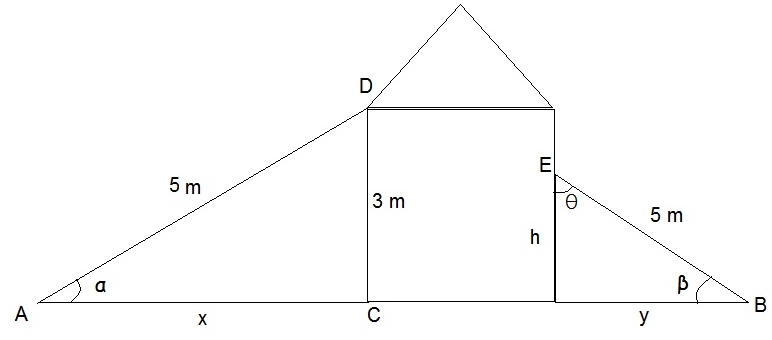
\includegraphics[width=0.45\textwidth]{vic_1_2.jpg}
%\centering\captionof{figure}{Preguntas \ref{vic-1} y \ref{vic-2}}\label{fig:vic-1-2}
%\justifying
\begin{enumerate}
\item En un paseo de grupo de estudiantes de grado 11$^o$, han armado una carpa que est\'a sujeta por dos cuerdas de 5 metros para darle mayor estabilidad. Tanto la cuerda A como la cuerda B  miden 5 metros y se sujetan de los puntos como se muestra. \label{vic-1}\\

La distancia x desde el punto A hasta el punto C es igual a:
\begin{enumerate}[(A)]
\item 8 m
\item 6 m 
\item 4 m 
\item 2 m
\end{enumerate}

\newpage
\item Si la cuerda B se sujeta de a la carpa a una altura h  y se sabe que el ángulo de elevación de la cuerda respecto a la horizontal es  $\beta$, entonces la altura h se puede expresar como:\label{vic-2}

\begin{enumerate}[(A)]
\item $5m x \sin\beta$
\item $5m x \cos\beta$
\item	$\frac{\sin\beta}{5}$
\item $\frac{\cos\beta}{5}$
\end{enumerate}
\item Un informe sobre el consumo de fruta de un grupo de niños durante la hora de descanso, lo hicieron de la siguiente \label{vic-3} manera:\\
50 comieron piña \\
40 - pera \\
30 - manzana\\
15 - ninguna\\
Pero debemos anotar que algunos comieron más de una fruta:\\
10 - piña y pera\\
5 - piña, pera y manzana\\
5 - piña y manzana\\
10 - pera y manzana\\
El número total de niños es:
\begin{enumerate}[(A)]
\item 80
\item 100
\item 120 
\item 135
\end{enumerate}


\begin{center}
\begin{table*}[htp]
%\begin{multicols}{1}
\begin{tabular}{|c|p{8.5cm}ccc|}
\hline 
PUESTO	&EDIFICIO	&PISOS	&ALTURA(m)	&AÑO\\
\hline \hline 
1	&Taipéi 101,Taipei(Taiwan)	&101	&509	&2004\\
2	&Petronas, Torres 1 Kuala Lumpur (Malasia)	&88	&452	&1998\\
3	&Petronas, Torres 1 Kuala Lumpur (Malasia)	&88	&452	&1998\\
4	&Torre Sears, Chicago (EE.UU)	&110	&442	&1974\\
5	&Edificio Jin Mao, Shanghai (China)	&88	&421	&1979\\
6	&Centro Int. de finanzas II, Hong Kong (China)	&88	&415	&2003\\
7	&Citic Plaza, Guangzhou (China)	&80	&391	&1996\\
8	&Shun Hing Square, Shenzhen (China)	&69	&384	&1996\\
9	&Edificio Empire State , New York (EE.UU)	&102	&381	&1931\\
10	&Central Plaza Hong Kong(China)	&78	&374	&1992\\
\hline 
\end{tabular} 
\captionof{table}{Tabla pregunta \ref{pregunta_altura}.}
%\end{multicols}

\end{table*}

\end{center}

\newpage


\item Se tiene la palabra impresiones, si se ponen en una bolsa cada letra y se saca una al azar, ¿cuál es la probabilidad de que la letra sacada sea una consonante? \label{vic-4} 
\begin{enumerate}[(A)]
\item $\frac{6}{11}$
\item $\frac{3}{11}$c
\item $\frac{1}{11}$
\item $\frac{8}{9}$
\end{enumerate}
\item El profesor Carlos pensando un ejercicio demora los 5/3 de un minuto; redactando el enunciado 4 minutos y 15 segundos; buscando los distractores 1/12 de hora y pasándolo a limpio 3 y $3/4$ de minuto.  ¿Qué tiempo empleó en elaborar 35 preguntas de una prueba de amptitud  matemática?\label{anexo_1}\label{vic-5}
\begin{enumerate}[(A)]
\item 12 h y 15 minutos.
\item 30.800 segundos.
\item 6.250 minutos.
\item 16 h. y 3 segundos.
\end{enumerate}



\item Antes  del siglo XIX, los edificios muy altos eran poco usuales, pero con la invención de diversos materiales como el acero y el hormigón, se hizo posible que iniciara la construcción de los primeros rascacielos. Desde su aparición hasta la actualidad, distintas potencias del mundo se han dado a la tarea de construir el edificio más alto del mundo. En este arduo proceso le han demostrado al mundo impactantes obras arquitectónicas. En la imagen se presenta una tabla con los datos de los 10 edificios más altos del todo el mundo.\label{vic-6} \label{pregunta_altura} \\

El edificio con menor altura por piso es:\hrulefill\\
\_\hrulefill\hrulefill\\
\_\hrulefill.

\item Se tiene un tanque cuya capacidad es de 32.480 litros. Está provisto de dos llaves: la llave A vierte 201 litros en 3 minutos. Y la llave B, 540 litros en 5 minutos; además tiene un desagüe C por el que escapan 240 litros en 8 minutos. El tiempo que tarda en llenarse del tanque, estando totalmente desocupada y abiertas las llaves y el desagüe, es: \label{vic-7}

\begin{enumerate}[(A)]
\item 3 h 44'
\item 3 h 68'
\item 4 h 33'
\item 4 h 73'
\end{enumerate}

\newpage
\item En las olimpiadas de matemáticas del Colegio Central se hacen 40 preguntas y cada pregunta correcta se premia con 5 puntos buenos; mientras que cada pregunta mal contestada se califica con tres puntos malos. Si contestando todas las preguntas el resultado es cero; las preguntas correctas fueron: \label{vic-8}
\begin{enumerate}[(A)]
\item 5
\item 15
\item 22
\item 25
\end{enumerate}
\item A un grupo de personas pertenecientes a un club de la tercera edad se le pregunto cuál era la actividad  que más le agradaba realizar sobre su permanencia en el club, de tres actividades posibles. Los resultados de la encuesta se presentan en la tabla que aparece en la imagen.\label{vic-9}

\begin{center}
\begin{tabular}{p{2cm}|p{1.8cm} p{2.5cm}}
\hline \hline 
Actividad	&Frecuencia Relativa	&Frecuencia\par relativa\par acumulada 	\\
\hline \hline 
Gimnasia	&12	&12	\\
Juegos de Mesa	&X	&W	\\
Leer	&9	&40	\\
\hline \hline 
\end{tabular} 
\end{center}

%\hrulefill\\
%\_\hrulefill\hrulefill\\
%\_\hrulefill.

\subsubsection*{Pregunta de selección múltiple con única respuesta. Responda con base en la siguiente información}

%\begin{flushleft}
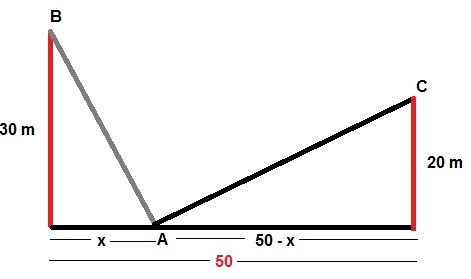
\includegraphics[width=0.45\textwidth]{vic_10.jpg} 
%\end{flushleft}
%\centering\captionof{figure}{Pregunta \ref{vic-10}}\label{fig:vic-10}
%\justifying

\newpage
\item Tenemos un poste de 30 metros de alturas y uno de 20 metros, la distancia entre ellos es de 50 metros. Se debe extender una cuerda que los une desde el extremo superior de cada uno de ellos. El centro de la cuerda debe tocar el piso. ¿a qué distancia del poste más bajo debe tocar el piso? \label{vic-10}\hrulefill\\
\_\hrulefill\hrulefill\\
\_\hrulefill.

%\begin{flushleft}

%\end{flushleft}
%\centering\captionof{figure}{Pregunta \ref{vic-11}}\label{fig:vic-11}
%\justifying
\item Se dice que una ventana es de estilo normando si tiene la forma de un cuadrado rematado por un semicírculo en la parte superior. Si r es el radio del semicírculo que está dada por $\frac{\pi r^2}{2}$  , y un cuadrado de radio $2r$, cuya área es igual a lado por lado, según la información suministrada el área de la ventana está dada por: \label{vic-11}

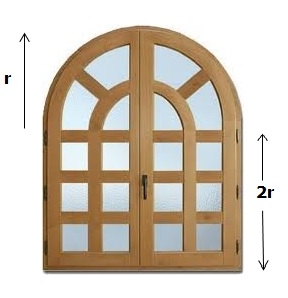
\includegraphics[width=0.45\textwidth]{vic_11.jpg} 

\begin{enumerate}[(A)]
\item $\frac{1}{4}r^2\pi+2r^2$
\item $\frac{\pi r^2}{2}+4r^2$
\item $r^2\pi+2r^2$
\item $\frac{1}{2}\pi+4r^2$
\end{enumerate}

\newpage
\subsubsection*{Pregunta de selección múltiple con única respuesta. Responda de acuerdo con la siguiente información}
\item Se realiza una convocatoria para unas vacantes en un circo y quedan seleccionado de la siguiente manera  hay 32 artistas, de estos 16 bailan, 25 cantan y 12 cantan y bailan. Según esto se desea saber el número de artistas que se incorporaron al circo que  no  cantan y bailan \label{anexo_conjuntos}\label{vic-12} 

\begin{enumerate}[(A)]
\item 10
\item 5
\item 8
\item 3
\end{enumerate}
\item En el curso de noveno  hay 30 estudiantes el 55\% tiene una nota en superior, el 35\% tiene notas en básico y el resto de las notas en bajo lo que quiere decir que están perdiendo la materia. \\ Entonces, el número de  estudiantes que están perdiendo es:\label{vic-13}
\begin{enumerate}[(A)]
\item 7
\item 13
\item 10
\item 3
\end{enumerate}

\newpage
%\begin{flushleft}
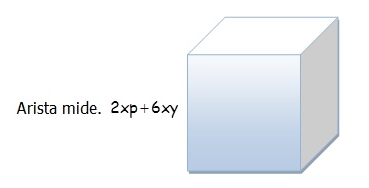
\includegraphics[width=0.4\textwidth]{vic_14.jpg} 
%\end{flushleft}
%\centering\captionof{figure}{Pregunta \ref{vic-14}}\label{fig:vic-14}
%\justifying

\item Se desea construir en el colegio un estanque para el estudio de especies acuáticas en la materia de Biología, si se sabe que  la expresión que representa el arista mide 2xp + 6xy, los estudiantes desean saber ¿Cuál de las siguientes les permitirá calcular el volumen total que ocupara el estanque? (Volumen del cubo es: Lado$^3$)\label{vic-14}


\begin{enumerate}[(A)]
\item $8x^{33}+72x^{32}y+213x^3y^2+216x^3y^3$
\item $8x^3p^3+72x^3p^2y+216x^3py^2+312x^3y^3$
\item $x^3p^3+x^3p^2y+x^3py^2+x^3y^3$
\item $216x^3+32py^2+16x^2yp^2+8p^3$
\end{enumerate}

\item Un almacén de televisores cuenta con 900 televisores de la marca A y 825 de marca B. Se debe distribuir todos los computadores en diferentes compañías de tal manera que todas reciban igual número de televisores marca A y todas reciban igual número de televisores marca B, el número máximo de compañías a las que se les puede hacer la distribución es:\label{vic-15}

\item En un hospital se a determinado que al enfermo lo visita la mamá todos los días, el papa día de por medio, una hermana cada 5 días, un hermano cada 15 días y una tía cada 18 días. Si para el 1 de enero con motivo del año nuevo se encontraron en el hospital, entonces la próxima fecha que se volverán a encontrar sabiendo que febrero tendrá 28 días es: \label{vic-16}

\begin{enumerate}[(A)]
\item 25
\item 75
\item 90
\item 180
\end{enumerate}

\item La siguiente tabla muestra las calificaciones obtenidas por un grupo de estudiantes universitarios, que se presentaron a un examen. \label{vic-17}


\begin{center}
\begin{tabular}[c]{|c|p{3cm}|}
\hline 
Calificaciones & Número de estudiantes  \\ 
\hline \hline
1 & 2	 \\ 
2 & 6 \\  
3 & 18 \\  
4 & 10 \\  
5 & 4 \\ 
\hline 
\end{tabular} 

\end{center}
¿Cuál es la gráfica que representa  la tabla de datos mostrada con  las calificaciones obtenidas?

\begin{enumerate}[(A)]
\item 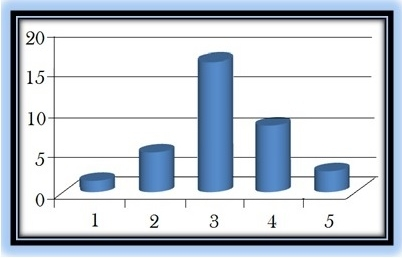
\includegraphics[width=0.3\textwidth]{vic_17_a.jpg} 
\item 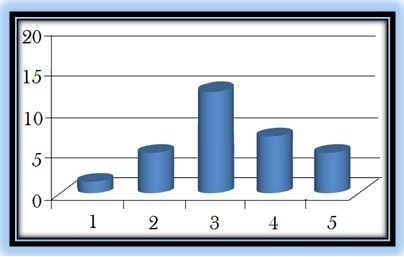
\includegraphics[width=0.3\textwidth]{vic_17_b.jpg} 
\item 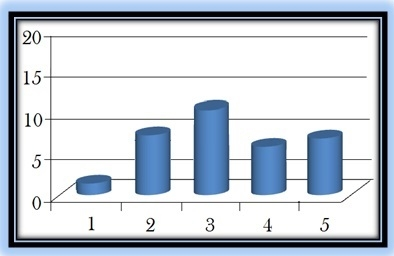
\includegraphics[width=0.3\textwidth]{vic_17_c.jpg} 
\item 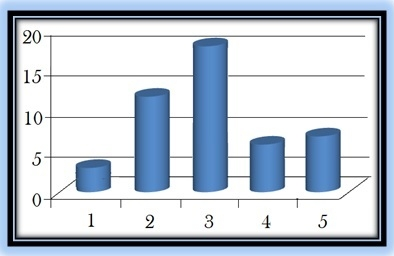
\includegraphics[width=0.3\textwidth]{vic_17_d.jpg} 
\end{enumerate}


\item  En un colegio de Bogotá hay 180 estudiantes repartidos por cada curso como se muestra en la tabla.\label{vic-18}

\begin{center}
\begin{tabular}{|c|cc|}
\hline 
 & Niñas & Niños \\ 
\hline \hline 
Primero & 30 & 15 \\ 
Segundo & 25 & 20 \\ 
Tercero & 27 & 18 \\ 
Cuarto & 33 & 12 \\ 
\hline 
\end{tabular} 
\end{center}


 Si se elige un estudiante al azar, ¿Cuál(es) de las siguientes proposiciones es (son) verdadera(s)?  
 \begin{enumerate}[I]
 \item I La probabilidad de que sea un niño es de $\frac{65}{180}$
\item La probabilidad de que se un estudiante de tercero es  $\frac{45}{180}$
\item La probabilidad de que sea una niña y de segundo es  $\frac{20}{45}$. 
 \end{enumerate}
\begin{enumerate}[(A)]
\item Sólo I
\item Sólo II
\item Sólo I y II
\item Sólo II y III
\end{enumerate}

 \item Tres personas practican natación diariamente de la siguiente forma:\label{vic-19}
Alejandro practica $2\frac{1}{2}$ horas, Patricia $3\frac{1}{4}$ horas y Ricardo $4\frac{3}{4}$ horas. 
¿Cuánto tiempo más práctico  Ricardo que Alejandro?

\begin{enumerate}[(A)]
\item 2 horas.
\item $2\frac{3}{8}$ horas.
\item 3 horas.
\item $2\frac{1}{4}$ horas.
\end{enumerate}
\newpage
\item Se quiere empacar 24 canicas rojas, 36 canicas azules  y  28  canicas amarillas  de tal forma que cada paquete contenga el mismo número de canicas de cada color. El número mínimo de paquetes que se necesita para realizar este empaque es:\label{vic-20}

\begin{enumerate}[(A)]
\item 24
\item 36
\item 6
\item 4
\end{enumerate}

\item Diana tiene contrato para vender azúcar al detal, en kilos (en dos bolsas), las ventas se incrementan diariamente de la siguiente manera progresiva: 8, 18, 28$\cdots$  \label{vic-21}

Al pasar un mes, y si el ritmo de las ventas no cambia, Diana puede decir que venderá cuantos kilos de azúcar:\hrulefill\\
\_\hrulefill\\
\_\hrulefill\\



\item Observa y analiza las siguientes gráficas:\label{vic-22}

%\begin{flushleft}
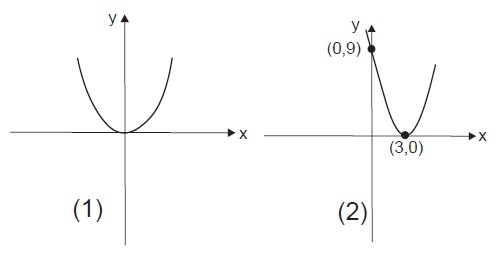
\includegraphics[width=0.45\textwidth]{vic_22.jpg} 
%\end{flushleft}
%\centering\captionof{figure}{Pregunta \ref{vic-22}}\label{fig:vic-22}
%\justifying

De acuerdo con las gráficas anteriores, se podría afirmar que, la gráfica (2) corresponde a la función:

\begin{enumerate}[(A)]
\item $y=x^2-3$
\item $y=x^2+3$
\item $y=(x+3)^2$
\item $y=(x-3)^2$
\end{enumerate}

\newpage
\item  Respecto a las gráficas de las funciones que se presentan a continuación se puede afirmar que: \label{vic-23}

%\begin{flushleft}
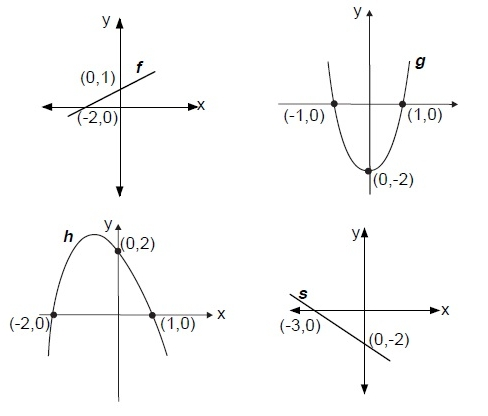
\includegraphics[width=0.45\textwidth]{vic_23.jpg} 
%\end{flushleft}
%\centering\captionof{figure}{Pregunta \ref{vic-23}}\label{fig:vic-23}
%\justifying

\begin{enumerate}[(A)]
\item Las funciones $f$ y $h$ interceptan al eje $y$ en el punto $(0, -2)$.
\item  Las funciones $g$ y $s$ interceptan al eje $x$ en el punto $(-2, 0)$.
\item  $f(1) = s(1) = 0$
\item $g(1) = h(1) = 0$ 
\end{enumerate}
\newpage
\item Observe la siguiente serie de igualdades: \label{vic-24}
\begin{align*}
&1+3=4\\
&1+3+5=9\\
&1+3+5+7=16\\
&1+3+5+7+9=25\\
&\vdots\\
&1+3+5+7+9+\cdots +(2n-1)=?
\end{align*}
Si $n$ es cualquier número natural, la suma $1+3+5+7+9+\cdots +(2n-1)$
es igual a: 
\begin{enumerate}[(A)]
\item $n^2$
\item $(2n-1)^2$
\item $(2n)^2$
\item $(n+1)^2$
\end{enumerate}


\newpage
\item En el sistema de coordenadas cartesianas que se muestra en la siguiente figura, se ha representado la trayectoria parabólica del salto de una rana. El desplazamiento horizontal que alcanza la rana en un salto es de 3 metros y la altura máxima es de 1 metro. \label{vic-25}

%\begin{flushleft}
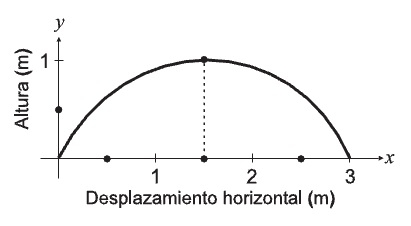
\includegraphics[width=0.45\textwidth]{vic_25.jpg} 
%\end{flushleft}
%\centering\captionof{figure}{Pregunta \ref{vic-25}}\label{fig:vic-25}
%\justifying

La ecuación que describe la trayectoria  del salto de la rana es:

\begin{enumerate}[(A)]
\item $y=-\left (x+\frac{3}{2}\right )^2+1$
\item $y=-\left (x-\frac{3}{2}\right )^2+1$
\item $y=-\frac{2}{3}x-\frac{5}{3}$
\item $y=-\frac{4}{9}x^2+\frac{4}{3}x$
\end{enumerate}

%%%%%%%%%%%%%%%%%%%%%%%%%%%%%
\end{enumerate}
%%%%%%%%%%%%%%%%%%%%%%%%%%%%%5

\newpage

\chapterimage{math2v.jpg} % Table of contents heading image

\chapter{Matemáticas II}\label{chap:math2}
\subsubsection*{Las preguntas del \ref{yolma-1} al \ref{yolma-3} se contestan con base en la siguiente información}


Un globo circular comienza a inflarse en un instante $t=0$; el radio de dicho globo en función del tiempo n, viene dado por la expresión $r (t)=2t+1$, donde $t$ representa el tiempo transcurrido en segundos y $r$ se mide en centímetros. Además debido a la calidad del caucho usado en la elaboración del globo, este explota cuando el diámetro del globo  alcanza 30 centímetros.\\
\begin{enumerate}

\item Con base en la información suministrada es válido afirmar que:\label{yolma-1}\\



\begin{enumerate}[(A)]
\item  En el instante en que empieza a ser llenado, el radio del globo es 2 centímetros
\item Por cada segundo transcurrido el volumen del globo aumenta en 2 centímetros cúbicos
\item El radio del globo y el tiempo transcurrido se comportan como magnitudes directamente proporcionales
\item Al momento de estallar el radio del globo es de 15 centímetros 
\end{enumerate}

%%%%%%%%%%%%%%%%%%%%%%%%%%%%%
\newpage
\item  El tiempo que transcurre desde el inicio del proceso de inflado hasta el instante en el cual el globo estalla es  \label{yolma-2}\\

\begin{enumerate}[(A)]
\item  30 segundos
\item 21 segundos
\item 15 segundos
\item 7 segundos
\end{enumerate}

%%%%%%%%%%%%%%%%%%%%%%%%%%%%%

\item  La expresión que permite determinar el volumen del globo, en función del tiempo transcurrido desde el inicio del proceso de inflado es \label{yolma-3}\\

\begin{enumerate}[(A)]
\item  Cuatro tercios de pi por radio al cubo
\item Cuatro tercios del radio al cubo
\item Cuatro veces el radio al cubo
\item Cuatro tercios de pi por el radio
\end{enumerate}

%%%%%%%%%%%%%%%%%%%%%%%%%%%%%
\subsubsection*{Responda las preguntas \ref{yolma-4} y \ref{yolma-5} de acuerdo a la siguiente información}

Los siguientes datos indica los valores obtenidos para dos funciones $f$ y $g$ al ser evaluados en $x=0$.  $f(0)=3$; $f’(0)=1$; $g(0)=2$; $g’(0)=1$


\newpage
\item Con base en la información suministrada es correcto afirmar que: \label{yolma-4}\\

\begin{enumerate}[(A)]
\item  La función $f$ no es diferenciable en $x=0$
\item Las funciones $f$ y $g$ son continuas en $x=0$
\item La función $g$ es diferenciable en $x=0$ pero no es continua
\item Tanto $f$ como $g$ no son diferenciables en $x=0$
\end{enumerate}

%%%%%%%%%%%%%%%%%%%%%%%%%%%%%

\item De acuerdo con la información suministrada se verifica que la función $f*g$ es diferenciable en $x=0$ y además, que $(f*g)’(0)$ es igual a \label{yolma-5}\\

\begin{enumerate}[(A)]
\item  5
\item 1
\item 6
\item 2
\end{enumerate}

%%%%%%%%%%%%%%%%%%%%%%%%%%%%%

\subsubsection*{Responda las preguntas \ref{yolma-6}  al \ref{yolma-9} con base en la siguiente información}

\noindent En el proceso de elaboración de un determinado materia, se estipula que dada una cantidad $M$, en kilogramos, de masa a procesar para obtener el material, la temperatura que alcanza el proceso viene dada por la expresión: 

\begin{equation*}
M^2+20M, \text{en grados centígrados}
\end{equation*}

Por razones de seguridad, la temperatura del proceso, no debe superar los 12.000 grados centígrados.

\newpage
\item La información dada en el texto, en términos de inecuaciones se expresa como:  \label{yolma-6}\\

\begin{enumerate}[(A)]
\item  $M^2+12.000\leq 20M$
\item $12.000\leq M^2+20M$
\item $12.000+20M\leq M^2$
\item $M^2+20M\leq 12.000$
\end{enumerate}

%%%%%%%%%%%%%%%%%%%%%%%%%%%%%

\item Con base en la información, se puede procesar 40Kg de masa. En tal caso, la temperatura que alcanza el proceso es:\label{yolma-7}\\

\begin{enumerate}[(A)]
\item  1.500 grados centígrados
\item 1.800 grados centígrados
\item 2.100 grados centígrados
\item 2.400 grados centígrados
\end{enumerate}

%%%%%%%%%%%%%%%%%%%%%%%%%%%%%

\item  Con base en la expresión que determina la temperatura, según la cantidad de materia procesada, se observa que a mayor cantidad de materia procesada,  la temperatura \label{yolma-8}\\

\begin{enumerate}[(A)]
\item  Aumenta directamente proporcional a la masa
\item Aumenta linealmente proporcional a la masa
\item Aumenta cuadráticamente proporcional a la masa
\item Aumenta en algunos casos y en otros no varia
\end{enumerate}

%%%%%%%%%%%%%%%%%%%%%%%%%%%%%

\newpage

\item Una información adicional, establece que con el objeto de reducir costos de producción, la temperatura mínima del proceso de producción debe ser 1.500 grados; por lo tanto para el proceso  la cantidad de materia para el proceso debe \label{yolma-9}\\

\begin{enumerate}[(A)]
\item  Menor a 50Kg porque así se economiza mas energía
\item Exactamente 50Kg porque es la cantidad de materia que permite que la temperatura sea 1.500 grados
\item Algo más de 50Kg porque la graduación de la maquina no es exacta
\item Mucho más de 50Kg porque los niveles de producción así lo exigen
\end{enumerate}

%%%%%%%%%%%%%%%%%%%%%%%%%%%%%

\subsubsection*{Responda las preguntas \ref{yolma-10} al \ref{yolma-12} de acuerdo a la siguiente información}

\begin{center}
\begin{tabular}{c|ccc}
\hline 
\hline 
 & Efectivo & Cheque & Tarjeta \\ 
\hline 
\hline 
Hombre & 28 & 60 & 37 \\ 
Mujer & 40 & 39 & 46 \\ 
\hline 
\hline 
\end{tabular} 
\end{center}
\item  De la información en la tabla es válido afirmar que: \label{yolma-10}\\

\begin{enumerate}[(A)]
\item  El número de mujeres encuestadas es superior al de hombres encuestados
\item La cantidad de personas encuestadas es desconocida
\item 68 de los encuestados pagaron sus compras en efectivo
\item El número de mujeres encuestadas es inferior a 110
\end{enumerate}

%%%%%%%%%%%%%%%%%%%%%%%%%%%%%
\newpage
\item De acuerdo con la tabla se infiere que la probabilidad de que una persona que realice una compra en el supermercado, sea mujer y cancele en efectivo es: \label{yolma-11}\\

\begin{enumerate}[(A)]
\item  40/125
\item 40/250
\item 28/40
\item 85/125
\end{enumerate}

%%%%%%%%%%%%%%%%%%%%%%%%%%%%%

\item La probabilidad de que un hombre pague con cheque, es mayor que la probabilidad que: \label{yolma-12}\\

\begin{enumerate}[(A)]
\item  Pague en efectivo o con tarjeta
\item Una mujer pague en efectivo o en cheque
\item Una mujer pague en efectivo o con tarjeta
\item Una mujer pague en cheque
\end{enumerate}

%%%%%%%%%%%%%%%%%%%%%%%%%%%%%

\item Los divisores de un numero son:\label{yolma-13}\\\hrulefill\\
\_\hrulefill\\
\_\hrulefill\\



%%%%%%%%%%%%%%%%%%%%%%%%%%%%%

\subsubsection*{Responda las preguntas \ref{yolma-14} al \ref{yolma-16} de acuerdo con la siguiente información}
Para una terna de ángulos $A$, $B$, y $C$ se verifican las siguientes relaciones:

\begin{gather*}
\text{Sen}(A)=\frac13; \text{Sen}(B)=\frac35; \text{Sen}(C)=\frac{5}{13}\\
\text{Cos}(A)=\frac{2\sqrt{2}}{3}; \text{Cos}(B)=\frac45; \text{Cos}(C)=\frac{12}{13}
\end{gather*}

Los tres ángulos son agudos

\newpage
\item  Con base en la información suministrada, para determinar el valor de Tan($B$), es necesario\label{yolma-14}\\

\begin{enumerate}[(A)]
\item  Multiplicar $\frac35$ por $\frac45$
\item Dividir $\frac45$ entre $\frac35$
\item Sumar $\frac35$ y $\frac45$
\item Dividir $\frac35$ entre $\frac45$
\end{enumerate}

%%%%%%%%%%%%%%%%%%%%%%%%%%%%%

\item A partir de la información suministrada, es posible determinar que el valor $\frac{12}{5}$ es equivalente a  \label{yolma-15}\\
\begin{enumerate}[(A)]
\item  Tan($A$)
\item Cot($B$)
\item Sec($C$)
\item Ninguna de las anteriores
\end{enumerate}

%%%%%%%%%%%%%%%%%%%%%%%%%%%%%
\item  Con base en la información suministrada, para determinar el valor de Sen($A+B$), es necesario determinar el resultado de: \label{yolma-16}
\begin{enumerate}[(A)]
\item  Sen($A$)+Sen($B$)
\item Sen($A$)Cos($B$)+Sen($B$)Cos($A$)
\item Sen($A$)Cos($B$)-Sen($B$)Cos($A$)
\item Sen($A$)-Sen($B$)
\end{enumerate}

%%%%%%%%%%%%%%%%%%%%%%%%%%%%%

\item  Las relaciones trigonométricas se establecen\label{yolma-17}\hrulefill\\
\_\hrulefill\\
\_\hrulefill
\_\hrulefill.


%%%%%%%%%%%%%%%%%%%%%%%%%%%%%

\item Si un cilindro y un cono de igual altura y radio se acoplan por sus bases es incorrecto afirmar que: \label{yolma-18}
\begin{enumerate}[(A)]
\item  El volumen total de la pieza es $\frac43$ del volumen del cilindro
\item El volumen del cilindro es tres veces el volumen del cono
\item El volumen del cono es tres veces el volumen del cilindro
\item La altura total de la pieza es el doble de la del cono
\end{enumerate}

%%%%%%%%%%%%%%%%%%%%%%%%%%%%%

\item El volumen es: \label{yolma-19}\hrulefill\\
\_\hrulefill\\
\_\hrulefill
\_\hrulefill.

%%%%%%%%%%%%%%%%%%%%%%%%%%%%%

\subsubsection*{Responda las preguntas \ref{yolma-20} al \ref{yolma-22} de acuerdo con la siguiente información}

Una empresa promotora de salud ofrece dos planes de afiliación: el primero, tiene un valor de \$800.000 anuales y el segundo la mitad del valor del primero, más \$12.000 por cada día de hospitalización.

\item Para una persona que dure hospitalizada mes y medio, tiene mayor beneficio económico con: \label{yolma-20}\\

\begin{enumerate}[(A)]
\item  El segundo plan porque paga menos dinero
\item El primer plan
\item Cualquiera de los planes le sirve
\item El segundo plan si el valor es una fracción del primero
\end{enumerate}

%%%%%%%%%%%%%%%%%%%%%%%%%%%%%

\item Si la fracción que determina el valor del segundo plan se cuadriplicara, el tiempo que podría permanecer una persona hospitalizada para obtener el mismo costo del primero sería: \label{yolma-21}\\

\begin{enumerate}[(A)]
\item  Menos de un mes
\item Un mes exactamente
\item Más de un mes
\item Hasta un año
\end{enumerate}

%%%%%%%%%%%%%%%%%%%%%%%%%%%%%
\newpage
\item Si la fracción que determina el valor del segundo plan disminuye su denominador que pasaría con respecto al primer plan durante dos meses de hospitalización: \label{yolma-22}\\

\begin{enumerate}[(A)]
\item  El día de hospitalización resultaría 50\% más costoso respecto del primer plan
\item El día de hospitalización resultaría igual de costoso que en el primero
\item El día de hospitalización seria casi el doble de costoso que en el primero
\item El día de hospitalización seria el triple de costoso del primero
\end{enumerate}

%%%%%%%%%%%%%%%%%%%%%%%%%%%%%

\item La razón de dos segmentos es: \label{yolma-23}\hrulefill\\
\_\hrulefill\\
\_\hrulefill
\_\hrulefill.


%%%%%%%%%%%%%%%%%%%%%%%%%%%%%
\newpage
\item La compañía Personal Teaching ofrece dos tipos de cursos en áreas no académicas diferentes. Para la semana entrante dispone de 60 horas de trabajo destinadas a dictar los dos cursos. Además como dichos cursos son los productos bandera de la compañía, a la gerencia le interesa utilizar las 60 horas disponibles de esa semana. El curso de cocina requiere 1.5 horas de trabajo para su montaje y el de música requiere 1.25 horas. La ecuación que relaciona la cantidad de cursos que se ofrecerán de cada uno con el total de horas disponibles es: \label{yolma-24}
\begin{enumerate}[(A)]
\item  $1.5C+1.25M=60$
\item $1.5C-1.25M=60$
\item $1.25M-1.25C=60$
\item $1.5C+1.5M=60$
\end{enumerate}

%%%%%%%%%%%%%%%%%%%%%%%%%%%%%

\item La trigonometría es: \label{yolma-25}\hrulefill\\
\_\hrulefill\\
\_\hrulefill
\_\hrulefill.

%%%%%%%%%%%%%%%%%%%%%%%%%%%%%
\end{enumerate}
%%%%%%%%%%%%%%%%%%%%%%%%%%%%%5




%%%%%%%%%%%%%%%%%%%%%%%%%%%%%%%%%%%%%%%%%%%%%%%%%%
%%%%%%%%%%%%     Ciencias Fisica %%%%%%%%%%%%%%
%%%%%%%%%%%%%%%%%%%%%%%%%%%%%%%%%%%%%%%%%%%%%%%%%%
\chapterimage{physics2.jpg} % Table of contents heading image

\chapter{F\'{i}sica I}\label{chap:phy1}
\begin{enumerate}


%%%%%%%%%%%%%%%%
\item Usain Bolt es un atleta jamaicano especialista en pruebas de velocidad, ostenta el record de velocidad por correr $100.0$ m en $10.0$ s, sin embargo el atleta afirma que puede recorrer la misma distancia en $9.4$ s, los analistas están seguros que puede superar sus marcas ya que el atleta baja su ritmo al final de la carrera cuando sabe que ha ganado. ¿Cuál es la velocidad máxima media del atleta? \label{dia-1}

\begin{enumerate}[(A)]
\item $10.0\frac{m}{s}$
\item $10.6\frac{m}{s}$
\item $11.0\frac{m}{s}$
\item $9.4\frac{m}{s}$
\end{enumerate}

%%%%%%%%%%%%%%%%%%%%%
\item Asuma que, para el record, al atleta le toma un segundo acelerar desde el reposo a su velocidad máxima media y faltando $2$ s para finalizar la carrera comienza a desacelerar constantemente. ¿Cuál es la magnitud de esta desaceleración?\label{dia-2}

\begin{enumerate}[(A)]
\item $-5.3 \frac{m}{s^2}$
\item $-5.0 \frac{m}{s^2}$
\item $+5.3 \frac{m}{s^2}$
\item $+5.0 \frac{m}{s^2}$
\end{enumerate}

%%%%%%%%%%%%%%%%%%%%%%%%
\newpage
\item Una gráfica correcta de este movimiento sería: \label{dia-3}\\

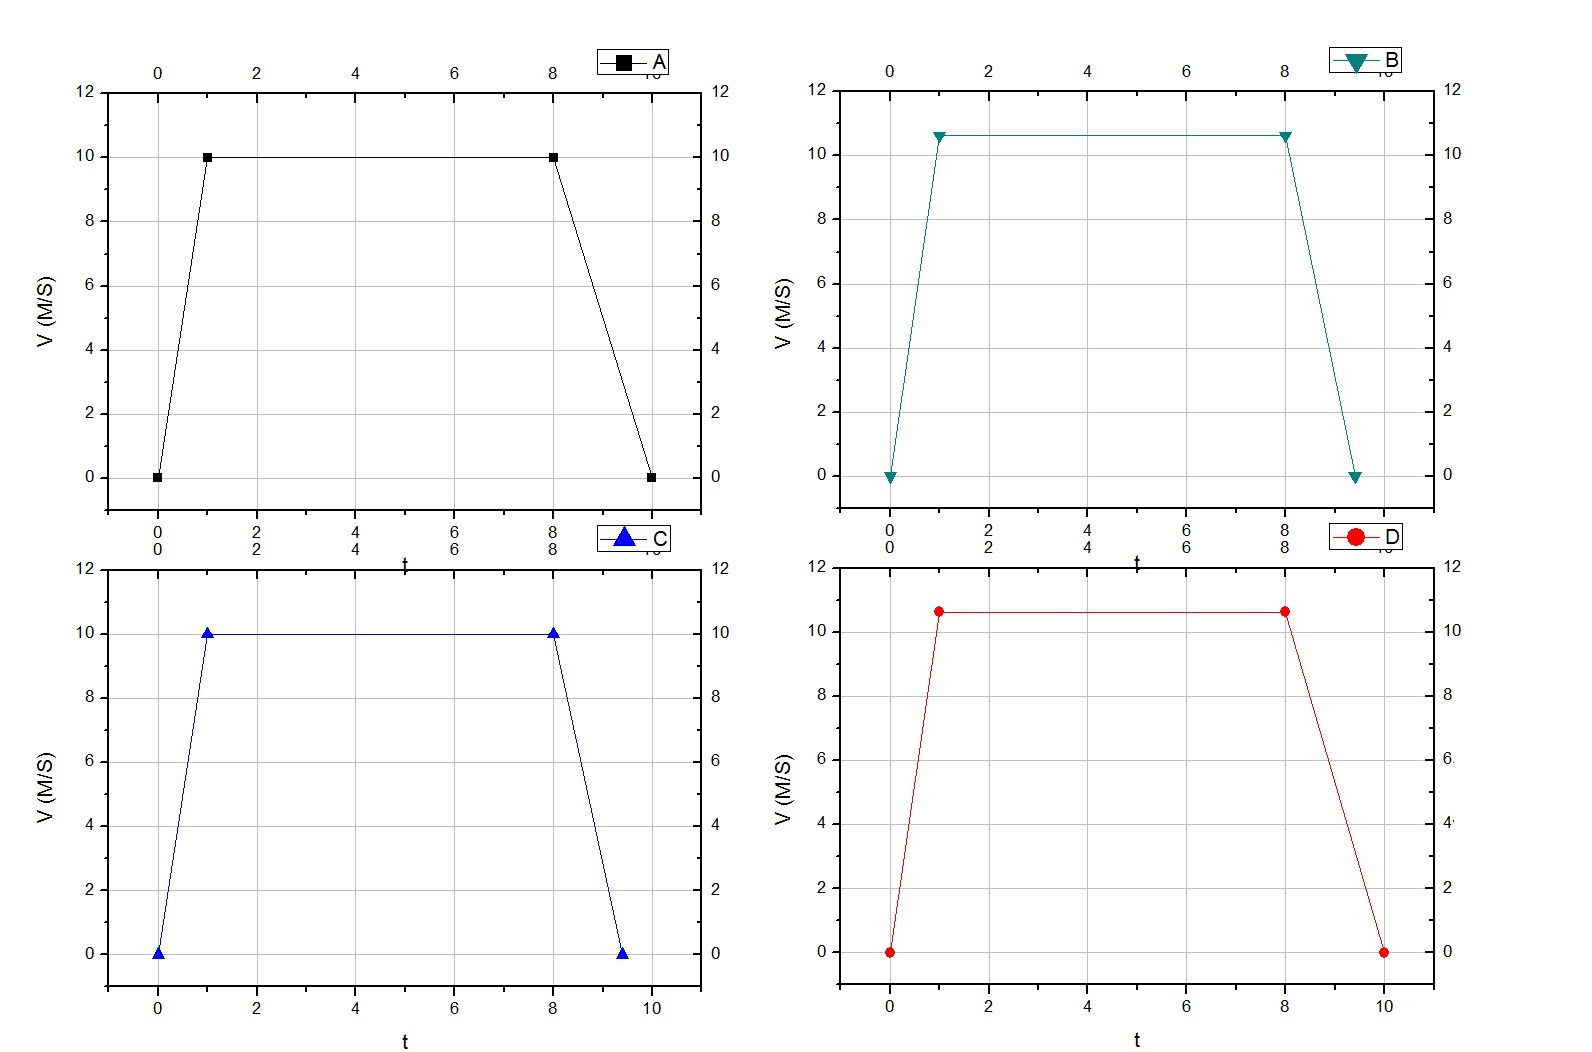
\includegraphics[width=0.45\textwidth]{dia1}


%%%%%%%%%%%%%%%%%%%%%%%%%

\item Supongamos que el atleta compite en un día con mucho viento, imagine que la velocidad del viento es aproximadamente $5.5\frac{m}{s}$, lastimosamente no supera su record y recorre $100$ m en $16$ s. \label{dia-4}
\noindent Una representación correcta con los valores dados en $\frac{m}{s}$ es:

% yo cambie el orden de la numeraciòn que tenia diana es decir cambie la figura llamada 2 y 1 por dia1 y dia2
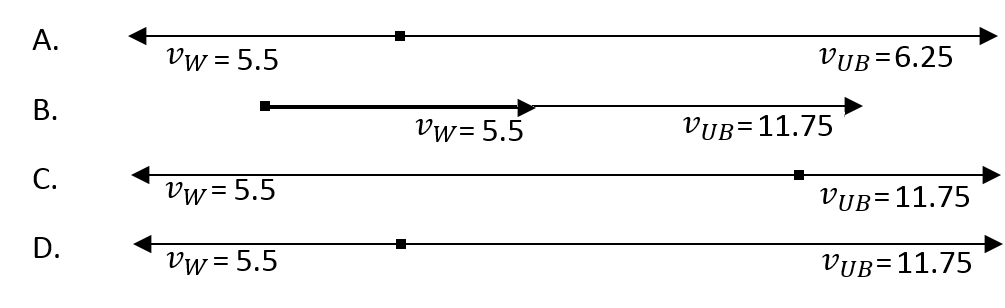
\includegraphics[width=0.45\textwidth]{dia2}

%%%%%%%%%%%%%%%%%%%%%%
\item Teniendo en cuenta lo anterior en un día sin viento, se hubiera superado el record? Justifique su respuesta claramente \label{dia-5} \hrulefill\\
\_\hrulefill\\
\_\hrulefill\\
\_\hrulefill.

%%%%%%%%%%%%%%%%%%%%%
\newpage
\item Thomas Muller, un futbolista alemán se encuentra practicando lanzando penaltis frente al arco de futbol. La distancia reglamentaria para cobrar un penalti es de $11$ m del arco, con un arco de $2.4$ m de altura. \label{dia-6}
\noindent ¿Cuál es la velocidad máxima vertical que debe imprimirle el jugador al balón para que haga gol? (Asuma que el balón tiene energía cinética nula en el eje Y)

\begin{enumerate}[(A)]
\item $4 \sqrt{2}\frac{m}{s}$
\item $4 \sqrt{3}\frac{m}{s}$
\item $4.0\frac{m}{s}$
\item Faltan datos en el problema
\end{enumerate}

%%%%%%%%%%%%%%%%%%%%%%%%%

\item ¿Cuánto tiempo dura el balón en el aire antes de conocer si es gol o no? (Recuerde que $\sqrt{3}>\sqrt{2}$) \label{dia-7}

\begin{enumerate}[(A)]
\item $0.56$ s
\item $0.69$ s
\item $0.40$ s
\item Faltan datos en el problema
\end{enumerate}

%%%%%%%%%%%%%%%%%%%%%%%%
\noindent Un tornamesa es un aparato para reproducir discos de vinilo. Asumamos uno de estos de $45$ RPM con un disco de $12$ pulgadas. 

\begin{center}
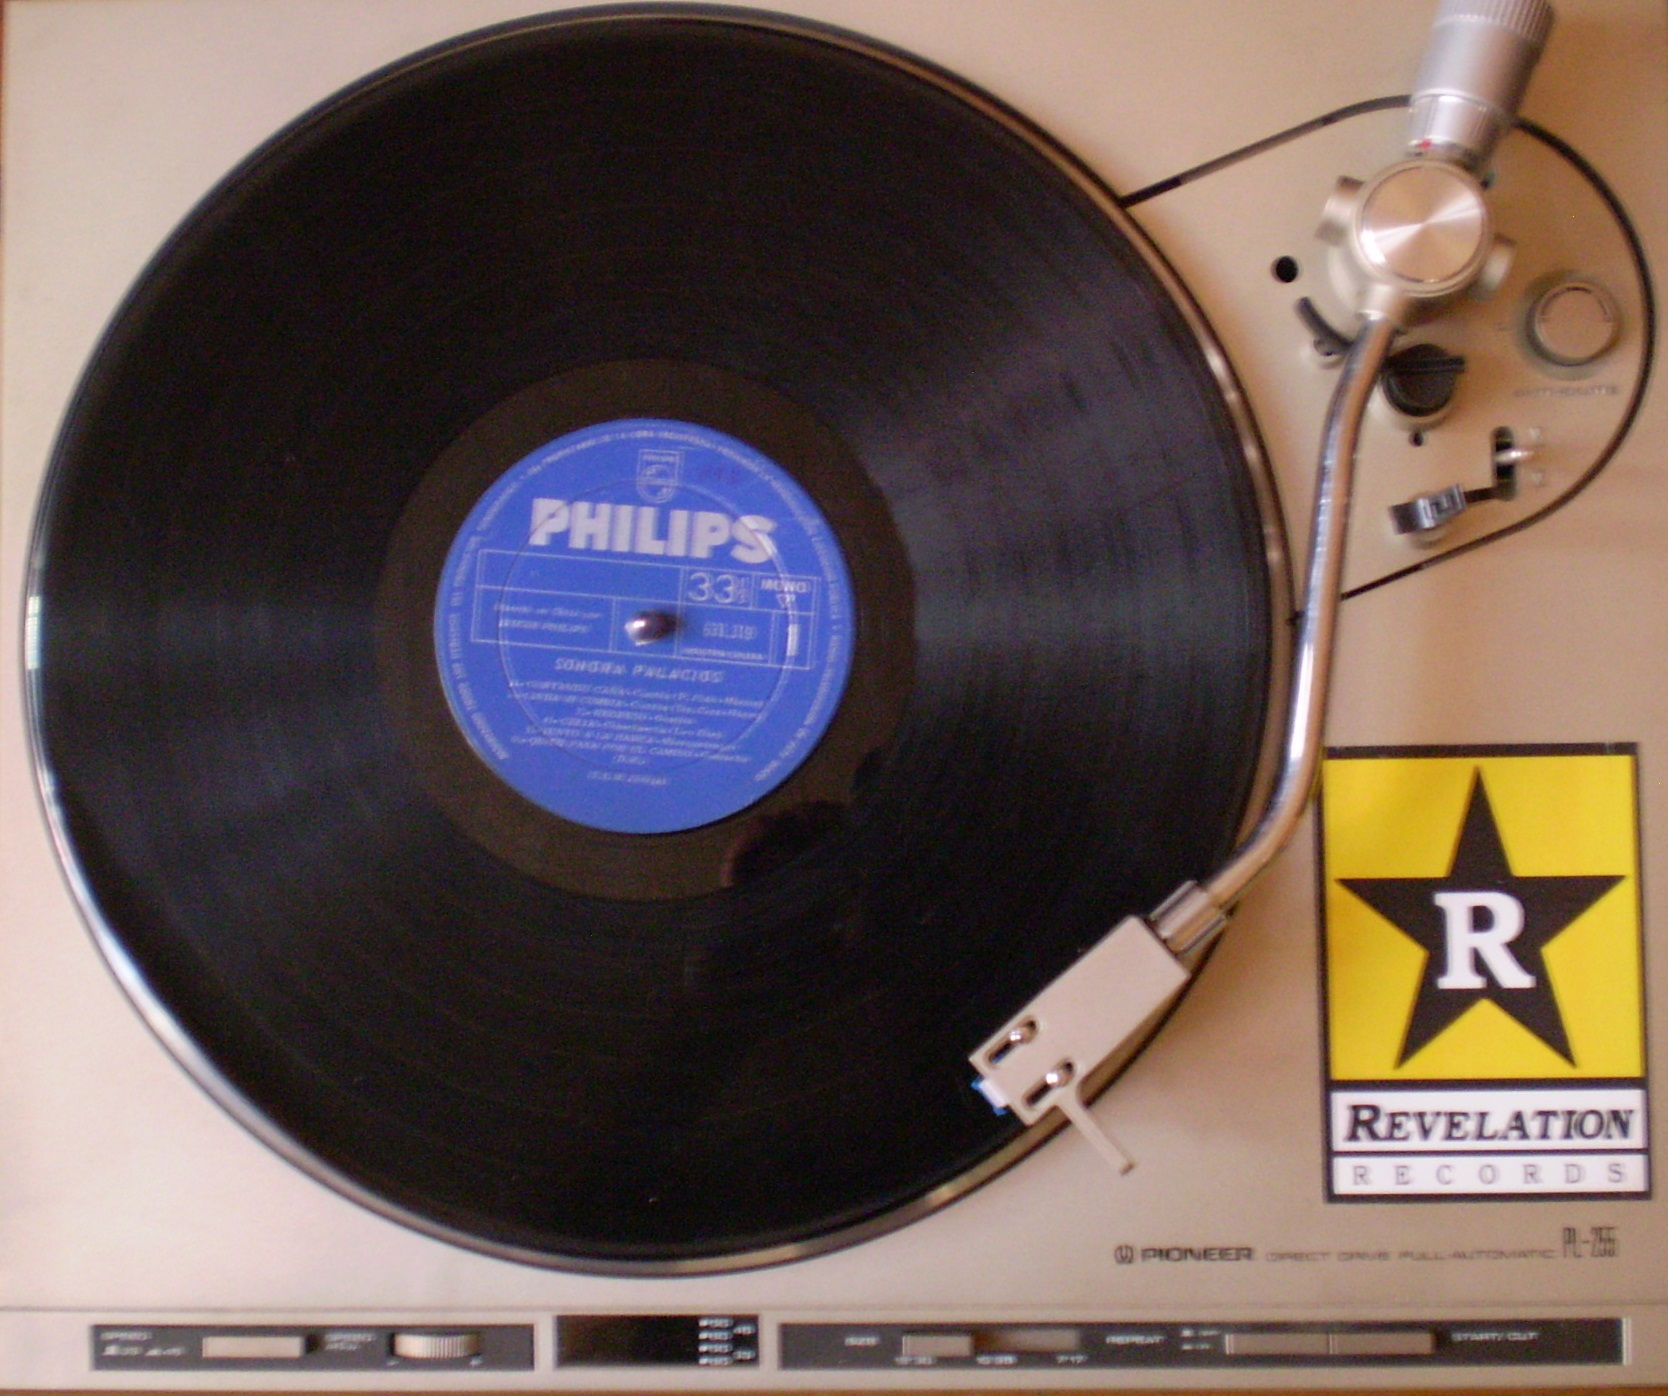
\includegraphics[width=0.35\textwidth]{dia3}
\end{center}

\newpage
\item ¿Cuál es la velocidad lineal de un punto situado en el borde del disco? \label{dia-8}

\begin{enumerate}[(A)]
\item $540\frac{m}{s}$
\item $32400\frac{pulg}{s}$
\item $540\frac{pulg}{s}$
\item $32400\frac{pulg}{min}$
\end{enumerate}

%%%%%%%%%%%%%%%%%%%%%%%

\item ¿Cuál es su aceleración centrípeta?\label{dia-9}

\begin{enumerate}[(A)]
\item $24300\frac{pulg}{s^2}$
\item $24300\frac{m}{s^2}$
\item $24300\frac{pulg}{min^2}$
\item $24300\frac{m}{min^2}$
\end{enumerate}

%%%%%%%%%%%%%%%%%%%%%%%
\item Cuando una esfera de plomo y una de madera de igual radio caen, la resistencia del aire $R$ que actúa sobre cada una de ellas es prácticamente igual. ¿Qu\'e se puede decir sobre las aceleraciones de las esferas?\label{dia-10}

\begin{enumerate}[(A)]
\item La esfera de plomo está más acelerada que la de madera
\item La esfera de plomo está menos acelerada que la de madera
\item Las aceleraciones son iguales
\item La resistencia del aire no cambia para nada el sistema
\end{enumerate}

%%%%%%%%%%%%%%%%%%%%%%%%%
\item En una campaña ecológica realizada se ha notado que si se vierte una gota de aceite de volumen $0.01cm^3$ sobre una piscina esta se expande uniformemente de tal manera que dicha capa tiene un espesor de $10^{-9}m$. ¿Cuál es el área de la piscina de agua contaminada?\label{dia-11}

\begin{enumerate}[(A)]
\item $1m^2$
\item $10m^2$
\item $100m^2$
\item $1000m^2$
\end{enumerate}

%%%%%%%%%%%%%%%%%%%%%%%%%%

\newpage
\item De acuerdo a lo anterior ¿cuántas piscinas de este mismo tamaño se contaminan con un litro de este aceite? \label{dia-12}

\begin{enumerate}[(A)]
\item 1000
\item 10000
\item 100000
\item 1 millon
\end{enumerate}

%%%%%%%%%%%%%%%%%%%%%%%%%
\item ¿Por qué los bomberos tienen que sujetar fuertemente la manguera cuando se lanza agua a alta presión para apagar un incendio? \label{dia-13} \hrulefill\\
\_\hrulefill\\
\_\hrulefill\\
\_\hrulefill.

%%%%%%%%%%%%%%%%%%%%%%%%%%%%

\item Un tubo de crema dental se cierra en la fábrica a la altura de mar y que se lleva un cargamento de estas a Bogotá para su comercialización. Cuando usted compre uno de estos tubos y lo abra la crema dental:\label{dia-14}

\begin{enumerate}[(A)]
\item Saldrá puesto que la presión de empacado es menor que la de sus condiciones actuales
\item Entrará puesto que la presión de empacado es menor que la de sus condiciones actuales
\item Saldrá puesto que la presión de empacado es mayor que la de sus condiciones actuales
\item Entrará puesto que la presión de empacado es mayor que la de sus condiciones actuales
\end{enumerate}

%%%%%%%%%%%%%%%%%%%%%%%%%%%%%
\newpage
\item Se tiene una pelota de $2$ Kg de masa a lo alto de una colina como se muestra en la situación.\label{dia-15}

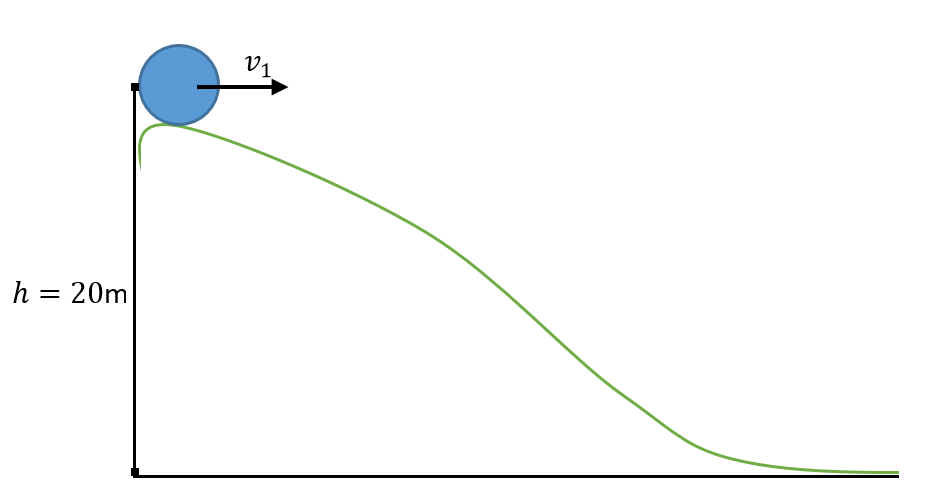
\includegraphics[width=0.45\textwidth]{dia4}

 ¿Cuál es el valor de la energía cinética al llegar al punto más bajo de la rampa? 

\begin{enumerate}[(A)]
\item $mgh$
\item $\frac{1}{2}mgh+\frac{mv_1^2}{2}$
\item $mgh+\frac{mv_1^2}{2}$
\item $mgh+mv_1^2$
\end{enumerate}

%%%%%%%%%%%%%%%%%%%%%%%%%%%%%%%

\item Tome en cuenta lo anterior y asuma que la pelota cae desde lo alto sin ninguna velocidad inicial ¿con qué velocidad llega al punto más bajo? \label{dia-16}

\begin{enumerate}[(A)]
\item $10\sqrt{2}\frac{m}{s}$
\item $20.0\frac{m}{s}$
\item $10.0\frac{m}{s}$
\item $2\sqrt{10}\frac{m}{s}$
\end{enumerate}

%%%%%%%%%%%%%%%%%%%%%%%%%%%%%%%%%%%
\item Una carreta de $20$ Kg se desplaza con una velocidad de $2\frac{m}{s}$. Un instante después una niña de $40$ Kg salta de la carreta con una velocidad en el mismo sentido de la carreta de $1\frac{m}{s}$, la nueva velocidad de la carreta es: \label{dia-17}

\begin{enumerate}[(A)]
\item $2.5\frac{m}{s}$
\item $3.5\frac{m}{s}$
\item $8.0\frac{m}{s}$
\item $4.0\frac{m}{s}$
\end{enumerate}

%%%%%%%%%%%%%%%%%%%%%%%%%%
\newpage
\item Un deposito muy grande de agua sujeto a presión atmosférica tiene un pequeño agujero sobre la pared lateral a una profundidad de $5$ m ¿Cuál es la velocidad de salida del agua? \label{dia-18}

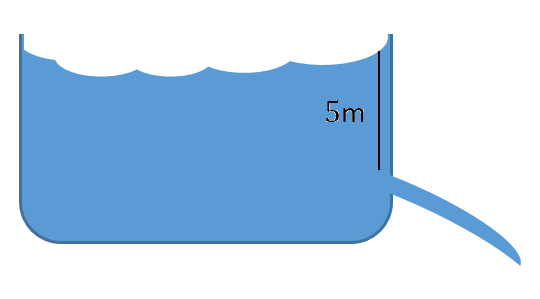
\includegraphics[width=0.45\textwidth]{dia5}

\begin{enumerate}[(A)]
\item $2\sqrt{5}\frac{m}{s}$
\item $5.0\frac{m}{s}$
\item $5\sqrt{2}\frac{m}{s}$
\item $10.0\frac{m}{s}$
\end{enumerate}

%%%%%%%%%%%%%%%%%%%%%%%%%%%%%
\item Un recipiente de $25cm^3$ (mostrado en la figura) contiene un líquido cuya densidad es $1200\frac{Kg}{m^3}$, se sumerge un sólido y $2/5$ partes de él flotan, determine la densidad del sólido. \label{dia-19}

\begin{enumerate}[(A)]
\item $720.0\frac{Kg}{m^3}$
\item $480.0\frac{Kg}{m^3}$
\item $240.0\frac{Kg}{m^3}$
\item No es posible determinarla
\end{enumerate}

%%%%%%%%%%%%%%%%%%%%%%%%%%%%%%
\item En medio de un bosque un leñador ve un relámpago y a los $5$ s escucha el trueno, $30$ s después se encuentra resguardado dentro de la cabaña ¿Cuál es la distancia entre el punto en el que cayó el rayo y la cabaña?\label{dia-20}\\
El sonido viaja aproximadamente a $340\frac{m}{s}$ y la luz a $300000\frac{Km}{s}$. 

\begin{enumerate}[(A)]
\item $10200$ Km
\item $170$ Km
\item $10200$ m
\item $1700$ m
\end{enumerate}


%%%%%%%%%%%%%%%%%%%%%%%%%%%%%%%%%
\item Un resorte con longitud natural $20$ cm, se alarga $5$ cm cuando se ejerce sobre él una fuerza de $2$ N. ¿Cuál es la constante elástica del resorte? \label{dia-21}

\begin{enumerate}[(A)]
\item $0.4\frac{N}{m}$
\item $0.1\frac{N}{m}$
\item $40\frac{N}{m}$
\item $10\frac{N}{m}$
\end{enumerate}

%%%%%%%%%%%%%%%%%%%%%%%%%%%%%%%%%
\item En un juego se tiene que mover una pelota pesada desde el reposo hasta una distancia máxima, uno de los jugadores tira la pelota de $5$ Kg a $25$ m en $5$ s. Asuma que la aceleración es constante, Cuál es la fuerza horizontal que el jugador ejerció sobre la pelota? \label{dia-22}

\begin{enumerate}[(A)]
\item $25$ N
\item $12.5$ N
\item $50$ N
\item $10$ N
\end{enumerate}

%%%%%%%%%%%%%%%%%%%%%%%%%%%%%%%%%
\item En una película de ciencia ficción una nave se encuentra en la mitad entre la Tierra y Marte cuando de repente un misil la golpea y se ve una explosión, un astronauta observando a la distancia puede ver la escena, pero ¿qué ruido siente?\label{dia-23}

\begin{enumerate}[(A)]
\item Ninguno
\item Uno que varía en intensidad dependiendo de la distancia a la cual se sitúe el astronauta
\item Uno idéntico al que se escucharía en la tierra pero más sordo 
\item Uno idéntico al que se escucharía en la tierra 
\end{enumerate}

%%%%%%%%%%%%%%%%%%%%%%%%%%%%%%%%%
\newpage

\item Dos recipientes cilíndricos abiertos en los cuáles se puede medir el nivel contienen el mismo líquido, se unen en la base por un tubo. En el cilindro 1 se vierte agua, como es posible que las medidas en los cilindros sean distintas? \label{dia-24}

\begin{enumerate}[(A)]
\item Inicialmente ambos estaban vacíos
\item Inicialmente contenían agua a distintos niveles
\item Inicialmente contenían un líquido distinto al agua
\item Tenían un diámetro distinto 
\end{enumerate}


%%%%%%%%%%%%%%%%%%%%%%%%%%%%%%%%%
\newpage
\item La luz es un tipo de onda \label{dia-25}
\begin{enumerate}[I.]
\item Transversal
\item Longitudinal
\item Electromagnética
\item Mecánica
\end{enumerate}


\begin{enumerate}[(A)]
\item I y III
\item I y IV
\item II y III
\item II y IV
\end{enumerate}



%%%%%%%%%%%%%%%%%%%%%%%%%%%%%
\end{enumerate}
%%%%%%%%%%%%%%%%%%%%%%%%%%%%%5



\chapterimage{physics3v.jpg} % Table of contents heading image

\chapter{F\'{i}sica II}\label{chap:phy2}
\subsubsection*{Las preguntas del \ref{yolf-1} al \ref{yolf-4} se contestan con base en la siguiente información}

\noindent La gráfica posición-tiempo para una figura que se mueve a lo largo del eje x se muestra en la figura:

\begin{center}
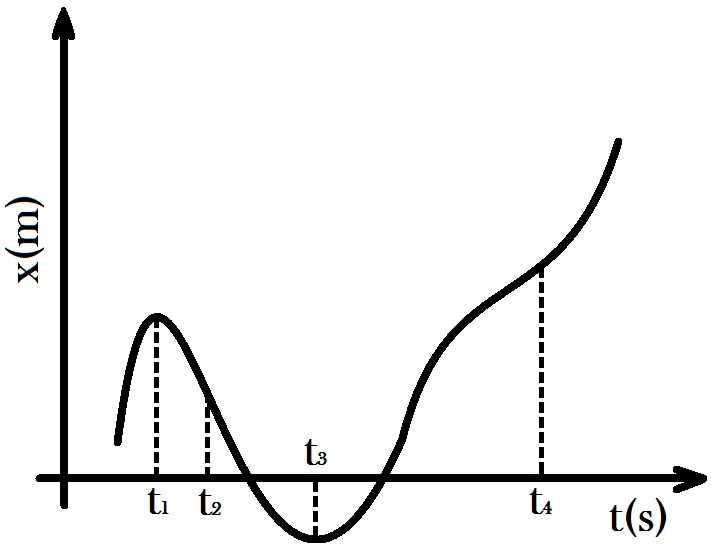
\includegraphics[width=0.45\textwidth]{yol_img1.jpg}
\end{center}



%%%%%%%%%%%%%%%%%%%%%%%%%%%%%%%%%%%
\begin{enumerate}
\item En $t_1$ la velocidad es 0 porque: \label{yolf-1}\\

\begin{enumerate}[(A)]
\item La pendiente de la recta tangente que es horizontal en ese punto es 0
\item  La curva ni crece ni decrece
\item  El cuerpo está en reposo
\item La aceleración es 0
\end{enumerate}


%%%%%%%%%%%%%%%%%%%%%%%%%%%%%%%%%%%
\newpage
\item En $t_2$ la velocidad es diferente de 0 pero negativa debido a:  \label{yolf-2}\\

\begin{enumerate}[(A)]
\item La pendiente de la recta tangente a la curva en ese punto es indeterminada
\item La pendiente de la recta tangente a la curva en ese punto es mayor que cero
\item  La pendiente de la recta tangente a la curva en ese punto es menor que cero
\item  La pendiente de la recta tangente a la curva en ese punto es igual a cero
\end{enumerate}

%%%%%%%%%%%%%%%%%%%%%%%%%%%%%%%%%%%
\item En $t_3$ la pendiente de la recta tangente a la curva es mayor que cero por tanto: \label{yolf-3}\\

\begin{enumerate}[(A)]
\item  La velocidad es indeterminada
\item  La velocidad es diferente de cero y positiva
\item La velocidad es diferente de cero y negativa
\item  La velocidad es igual a cero
\end{enumerate}

%%%%%%%%%%%%%%%%%%%%%%%%%%%%%%%%%%%
\newpage
\item  En $t_4$ la velocidad es igual a\label{yolf-4}\\

\begin{enumerate}[(A)]
\item La velocidad en $t_1$ porque las rectas tangentes a la curva en $t_1$ y en $t_4$ son paralelas y su pendiente es igual a cero
\item  La velocidad en $t_2$ porque las rectas tangentes a la curva en $t_2$ y en $t_4$ son perpendiculares y el producto de sus pendientes es -1
\item  La velocidad en $t_3$ porque las rectas tangentes a la curva en $t_3$ y en $t_4$ son horizontales
\item  Ninguno de los puntos marcados

\end{enumerate}

\subsubsection*{Las preguntas del \ref{yolf-5} al \ref{yolf-8} se contestan de acuerdo a la siguiente información:}

\noindent La figura muestra una gráfica de v contra t para el movimiento de un motociclista desde que parte del reposo y se mueve a lo largo de un camino en línea recta:

\begin{center}
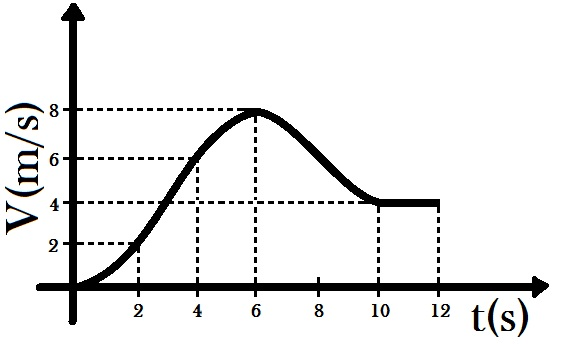
\includegraphics[width=0.45\textwidth]{yol_img2.jpg}
\end{center}

%%%%%%%%%%%%%%%%%%%%%%%%%%%%%%%%%%%
\item  La aceleración promedio puede ser calculada mediante la expresión: \label{yolf-5}\\

\begin{enumerate}[(A)]
\item  $a= v(0)-\frac{v(6)}{0-6}$
\item  $a= v(6)-\frac{v(0)}{6-0}$
\item  $a= \frac{0-6}{v(6)}-v(0)$
\item $a=\frac{6-0}{v(0)}-v(6)$

\end{enumerate}

%%%%%%%%%%%%%%%%%%%%%%%%%%%%%%%%%%%
\item El tiempo en el cual la aceleración tiene su mayor valor positivo y su valor en ese instante es: \label{yolf-6}\\

\begin{enumerate}[(A)]
\item  En $t=1$ y su valor es 1.1 $\frac{m}{s^2}$
\item  En $t=2$ y su valor es 2.2 $\frac{m}{s^2}$
\item  En $t=3$ y su valor es 1.3 $\frac{m}{s^2}$
\item  En $t=4$ y su valor es  2.2 $\frac{m}{s^2}$
\end{enumerate}

%%%%%%%%%%%%%%%%%%%%%%%%%%%%%%%%%%%
\item  La aceleración es 0 en $t=6$ y en $t=11$ porque: \label{yolf-7}\\

\begin{enumerate}[(A)]
\item  Las rectas tangentes a la curva son horizontales
\item  Las pendientes de las tangentes a la curva en esos puntos son iguales a 0
\item  Las pendientes son oblicuas y diferentes de 0
\item  Las opciones a y b son correctas
\end{enumerate}

%%%%%%%%%%%%%%%%%%%%%%%%%%%%%%%%%%%
\item  En $t=8$ la aceleración tiene un valor de -1.3$\frac{m}{s^2}$ , este valor es: \label{yolf-8}\\

\begin{enumerate}[(A)]
\item  El máximo valor positivo
\item  El máximo valor negativo
\item  El mínimo valor positivo
\item  El mínimo valor negativo
\end{enumerate}

\newpage
\subsubsection*{Las preguntas \ref{yolf-9} al \ref{yolf-12} se contestan de acuerdo a la siguiente información:}


\noindent Cada uno de los vectores de desplazamiento A y B mostrados en la figura tiene una magnitud de 3 metros

\begin{center}
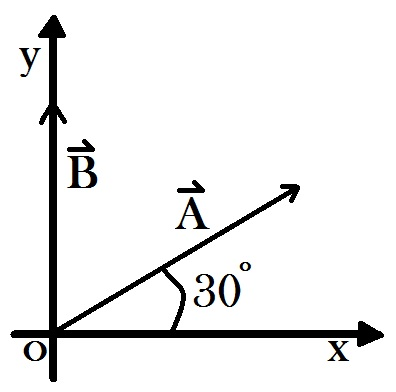
\includegraphics[width=0.3\textwidth]{yol_img3.jpg}
\end{center}
%%%%%%%%%%%%%%%%%%%%%%%%%%%%%%%%%%%
\item  La figura representa \label{yolf-9}\\

\begin{center}
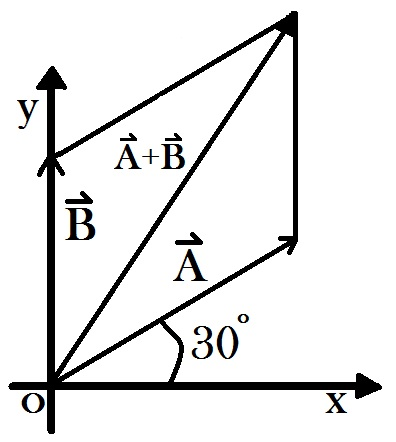
\includegraphics[width=0.3\textwidth]{yol_img4.jpg}
\end{center}

\begin{enumerate}[(A)]
\item  La suma de los vectores $\vec{A}$  y $\vec{B}$ por el método grafico
\item  La suma de los vectores $\vec{A}$  y $\vec{B}$ por el método del triangulo
\item  La suma de los vectores $\vec{A}$  y $\vec{B}$ por el método del paralelogramo
\item  La suma de los vectores $\vec{A}$  y $\vec{B}$ por el método de las componentes rectangulares
\end{enumerate}

%%%%%%%%%%%%%%%%%%%%%%%%%%%%%%%%%%%
\newpage
\item El vector $\vec{A}-\vec{B}$ \label{yolf-10}
\begin{center}
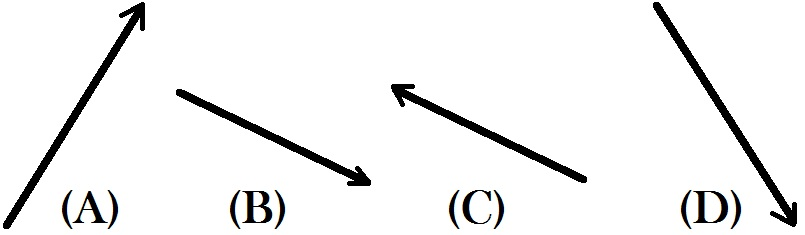
\includegraphics[width=0.45\textwidth]{yol_img5.jpg}
\end{center}

%%%%%%%%%%%%%%%%%%%%%%%%%%%%%%%%%%%
\item El vector $\vec{D}$ de la figura anterior representa \label{yolf-11}\\

\begin{enumerate}[(A)]
\item  $\vec{A}-\vec{B}$
\item  $\vec{A}+\vec{B}$
\item  $\vec{B}-\vec{A}$
\item  $\vec{A}-\vec{2B}$
\end{enumerate}

%%%%%%%%%%%%%%%%%%%%%%%%%%%%%%%%%%%
\item La magnitud del vector suma es  \label{yolf-12}\\

\begin{enumerate}[(A)]
\item  6 unidades en cualquier caso
\item  Mayor a 6 unidades si los vectores estuvieran sobre los ejes del plano
\item  Menor a 6 unidades
\item  Mayor a 6 unidades
\end{enumerate}

%%%%%%%%%%%%%%%%%%%%%%%%%%%%%%%%%%%
\item El trabajo se define como \label{yolf-13}\hrulefill\\
\_\hrulefill\\
\_\hrulefill\\
\_\hrulefill.


%%%%%%%%%%%%%%%%%%%%%%%%%%%%%%%%%%%
\item La relación entre el trabajo y la energía cinética se puede expresar como \label{yolf-14}\\

\begin{enumerate}[(A)]
\item  La suma de las energías cinéticas inicial y final
\item  La diferencia entre la energía cinética inicial y la energía cinética final
\item  La diferencia entre la energía cinética final y la energía cinética inicial
\item  El producto de las energías cinéticas inicial y final
\end{enumerate}

%%%%%%%%%%%%%%%%%%%%%%%%%%%%%%%%%%%
\item La potencia se define como \label{yolf-15}\hrulefill\\
\_\hrulefill\\
\_\hrulefill\\
\_\hrulefill.

%%%%%%%%%%%%%%%%%%%%%%%%%%%%%%%%%%%
\item La energía química de los alimentos se puede considerar como \label{yolf-16}\\

\begin{enumerate}[(A)]
\item  Energía cinética
\item  Energía potencial
\item  Energía potencial gravitacional
\item  Energía potencial elástica
\end{enumerate}

%%%%%%%%%%%%%%%%%%%%%%%%%%%%%%%%%%%
\item Con respecto al impulso se puede decir que \label{yolf-17}\\
\begin{enumerate}[(A)]
\item  Es el cambio en la velocidad porque al impulsarse la velocidad aumenta
\item  Es el cambio en la aceleración porque actúa la fuerza
\item  Es el cambio de la fuerza con relación al tiempo porque la fuerza es un vector
\item  Es el cambio en la cantidad de movimiento porque depende tanto d la masa como de la velocidad
\end{enumerate}

%%%%%%%%%%%%%%%%%%%%%%%%%%%%%%%%%%%
\item  Son elementos de una onda excepto \label{yolf-18}\\

\begin{enumerate}[(A)]
\item  Cresta ,valle y ciclo
\item  Difracción, interferencia y reflexión
\item  Amplitud, frecuencia y periodo
\item  Nodo, longitud de onda y velocidad de onda
\end{enumerate}

%%%%%%%%%%%%%%%%%%%%%%%%%%%%%%%%%%%
\item  La termodinámica es la rama de la física que \label{yolf-20}\hrulefill\\
\_\hrulefill\\
\_\hrulefill\\
\_\hrulefill.


%%%%%%%%%%%%%%%%%%%%%%%%%%%%%%%%%%%
\newpage
\item  Del sonido no se puede decir que  \label{yolf-19}\\

\begin{enumerate}[(A)]
\item  Es un fenómeno que involucra la propagación en forma de ondas elásticas
\item  Las ondas audibles producen oscilaciones en la presión del aire y las convierte en ondas mecánicas percibidas por el oído
\item  La propagación del sonido involucra transporte de energía y de materia
\item  Para que se genere un sonido es necesario que vibre alguna fuente
\end{enumerate}



%%%%%%%%%%%%%%%%%%%%%%%%%%%%%%%%%%%
\item   La primera ley de la termodinámica permite definir el calor como \label{yolf-21}\\

\begin{enumerate}[(A)]
\item  Un cambio en el trabajo sobre un sistema
\item  La energía necesaria que debe intercambiar un sistema para compensar las diferencias entre trabajo y energía interna
\item  Un cambio en la temperatura de un sistema
\item  Un cambio en la dirección en la que deben llevarse a cabo los procesos termodinámicos
\end{enumerate}
%%%%%%%%%%%%%%%%%%%%%%%%%%%%%%%%%%%
\item  Con respecto a las interacciones eléctricas no se puede concluir que. \label{yolf-22}\\

\begin{enumerate}[(A)]
\item  Son mucho más intensas que las interacciones gravitatorias
\item  Las cargas eléctricas pueden ser positivas o negativas
\item  Las interacciones entre las cargas eléctricas pueden ser atractivas o repulsivas
\item  La carga eléctrica constituye una medida de la estructura eléctrica de los átomos
\end{enumerate}

%%%%%%%%%%%%%%%%%%%%%%%%%%%%%%%%%%%
\item  La inercia es: \label{yolf-23}\hrulefill\\
\_\hrulefill\\
\_\hrulefill\\
\_\hrulefill.





%%%%%%%%%%%%%%%%%%%%%%%%%%%%%%%%%%%
\item   El voltaje se relaciona con: \label{yolf-25}\hrulefill\\
\_\hrulefill\\
\_\hrulefill\\
\_\hrulefill.


\newpage
%%%%%%%%%%%%%%%%%%%%%%%%%%%%%%%%%%%
\item   Un fluido se caracteriza por: \label{yolf-24}\\

\begin{enumerate}[(A)]
\item  Ser un medio que se mueve
\item  Su incapacidad para resistir esfuerzos cortantes
\item  Carecer de forma definida
\item  La opción b y c son correctas
\end{enumerate}

%%%%%%%%%%%%%%%%%%%%%%%%%%%%%
\end{enumerate}
%%%%%%%%%%%%%%%%%%%%%%%%%%%%%5



%%%%%%%%%%%%%%%%%%%%%%%%%%%%%%%%%%%%%%%%%%%%%%%%%%
%%%%%%%%%%%%     Ciencias Sociales %%%%%%%%%%%%%%
%%%%%%%%%%%%%%%%%%%%%%%%%%%%%%%%%%%%%%%%%%%%%%%%%%

\chapterimage{sociales1v.jpg} % Table of contents heading image

\chapter{Ciencias Sociales I}\label{chap:soc1}


\subsubsection*{Con base en el siguiente texto responda las preguntas: \ref{socandres-1} a \ref{socandres-3}}
Hasta el siglo XV América fue un continente habitado mayoritariamente por indígenas de diversas culturas: Mayas, Aztecas, Chibchas, Incas, etc. No obstante, se dice en algunos libros de historia que en 1492 surge el llamado ``descubrimiento de América''. El diccionario de la Real Academia Española define ``descubrimiento'' como: ``Hallazgo, encuentro, manifestación de lo que estaba oculto o secreto o era desconocido''.

\begin{enumerate}
\item Lo anterior presupone una paradoja porque: \label{socandres-1}

\begin{enumerate}[(A)]
\item 1492 es un año que está inserto dentro del siglo XV.
\item La definición de la Real Academia Española no contempla hechos históricos.
\item No se puede descubrir algo que ya ha sido descubierto por otros.
\item No se puede determinar exactamente quién descubrió América.
\end{enumerate}


%%%%%%%%%%%%%%%%%%%%%
\newpage
\item Una explicación acertada para este fenómeno es\label{socandres-2}
\begin{enumerate}[(A)]
\item La fuerza de la costumbre ha configurado el contenido de algunos libros de historia.
\item Colón pensaba que llegaba a las Indias descubriendo accidentalmente América.
\item Los recursos informativos en el siglo XV eran escasos y por ende no pudieron hacer un rastreo histórico exacto.
\item Dichos libros de historia manejan una perspectiva Eurocéntrica.
\end{enumerate}

\item Justifique su respuesta \label{socandres-3} \hrulefill\\
\_\hrulefill\\
\_\hrulefill\\
\_\hrulefill.

\subsubsection{Responda las preguntas de la \ref{socandres-4} a la \ref{socandres-6} con base en el siguiente texto.}
``A los cincuenta años \rule{3cm}{1pt} interviene por primera vez en la historia de la inquisición española. <<Mi nombre es Liberación>>, le hace exclamar Víctor Hugo. La realidad es bastante diferente y más desgraciada, atribuyéndosele la responsabilidad de muchas muertes de herejes.''\\{\footnotesize Tomado de: De Juan, J. y Pérez, F. (1985) La inquisición. Editora Cinco S.A. Bogotá. Pág. 35.}

\item El anterior texto hace referencia a un personaje histórico conocido como el primer gran inquisidor o primer inquisidor general, el cual es: \label{socandres-4}

\begin{enumerate}[(A)]
\item Fray José de Ascanio, nacido en 1210.
\item Papa Pío VI (Ángelo Onofrio), nacido en 1717.
\item Fray Tomás de Torquemada, nacido en 1420.
\item Papa Rodrigo Borgia (Alejandro VI), nacido en 1431. 
\end{enumerate}

\item El principal objetivo de la inquisición fue:\label{socandres-5}
\begin{enumerate}[(A)]
\item Torturas selectivas a los desertores de la Santa Iglesia Católica.
\item Supresión de la herejía, principalmente en el seno de la Santa Iglesia Católica.
\item Luchas cruzadas en contra de fundamentalistas de otras religiones.
\item Acaparamiento del oro proveniente de la recién descubierta América, por parte de la Santa Iglesia Católica. 
\end{enumerate}

\item La Inquisición es una institución que históricamente ha despertado fuertes críticas en diversos sectores debido a:\label{socandres-6}
\begin{enumerate}[(A)]
\item La ausencia de radicalismo en los procedimientos para la supresión de la herejía.
\item El acaparamiento de las riquezas de pueblos periféricos en torno a la figura del Papa.
\item Extralimitaciones en los procedimientos para combatir la herejía como el asesinato, la tortura y otros crímenes.
\item La falta de tolerancia ante las ideas religiosas profesadas por las comunidades musulmanas y asiáticas.
\end{enumerate}

\subsubsection*{Responda las preguntas de la \ref{socandres-7} a la \ref{socandres-10} con base en el siguiente texto}
``La condición esencial de la existencia y de la dominación de la clase burguesa es la acumulación de la riqueza en manos de particulares, la formación y el acrecentamiento del capital. La condición de existencia del capital es el trabajo asalariado. El trabajo asalariado descansa exclusivamente sobre la competencia de los obreros entre sí. El progreso de la industria, del que la burguesía, incapaz de oponérsele, es agente involuntario, sustituye el aislamiento de los obreros, resultante de la competencia, por su unión revolucionaria mediante la asociación. Así, el desarrollo de la gran industria socava bajo los pies de la burguesía las bases sobre las que ésta produce y se apropia lo producido. La burguesía produce, ante todo, sus propios sepultureros.''\\
\begin{footnotesize}
Tomado de: Marx Karl, Engels F. (1970) Manifiesto del partido comunista y otros escritos políticos. Editorial Grijalbo. México, D.F. Pág. 38.
\end{footnotesize}

\item Con la frase: “La condición esencial de la existencia y de la dominación de la clase burguesa es la acumulación de la riqueza en manos de particulares” Marx se refiere a:\label{socandres-7}

\begin{enumerate}[(A)]
\item Que es requisito para la constitución de una sociedad burguesa el atesoramiento de las riquezas por parte de una clase social determinada.
\item Que sólo a través de la apropiación y acumulación de la riqueza por parte de la clase burguesa puede ésta existir y mantener su dominio.
\item Que la burguesía para mantener su existencia y dominio debe impedir la existencia de una esfera pública social determinada.
\item Que la burguesía constituye en sí misma un modo de producción determinado puesto que el atesoramiento de la riqueza se da únicamente en su respectiva clase social.
\end{enumerate}

\item De la frase: “El trabajo asalariado descansa exclusivamente sobre la competencia de los obreros entre sí”, se podría concluir que:\label{socandres-8}

\begin{enumerate}[(A)]

\item Los obreros deben competir entre ellos mismos en la producción de bienes puesto que de ello dependerá el monto y renta de su salario.
\item Los obreros deben competir entre ellos mismos para asegurar un lugar dentro del sistema de producción y con ello un salario y su subsistencia.
\item Los obreros deben competir para obtener un lugar dentro del ejército de reserva industrial y de esta manera asegurar su subsistencia.
\item Los obreros deben competir entre sí en la rapidez mecánica de su ejercicio laboral para dar paso a nuevas formas de producción.
\end{enumerate}


\item Según los planteamientos de Karl Marx, el sistema capitalista es:\label{socandres-10}

\begin{enumerate}[(A)]
\item Justo, porque toda persona recibe una retribución o salario que se establece conforme al trabajo realizado.
\item Injusto, porque se sostiene sobre la explotación de los trabajadores a raíz, principalmente, de la apropiación de la plusvalía por parte de la burguesía.
\item Justo, porque el ser burgués o proletario no es algo inmanente a la naturaleza humana, sino que dependerá del esfuerzo de cada sujeto.
\item Injusto, porque no se combate la desigualdad inherente a la naturaleza humana.
\end{enumerate}


%%%%%%%%%%%%%%%%%%%%%%%%5
\newpage
\item Cuando Marx afirma que: “El progreso de la industria, del que la burguesía, incapaz de oponérsele, es agente involuntario, sustituye el aislamiento de los obreros, resultante de la competencia, por su unión revolucionaria mediante la asociación.” Se puede inferir que:\label{socandres-9}

\begin{enumerate}[(A)]
\item Con el necesario progreso de la industria, es inevitable que los obreros se aglutinen en fábricas y de esta manera, al permanecer juntos e identificar una explotación conjunta -como clase proletaria- se asocien con el fin de transformar sus condiciones materiales de vida a través de una revolución que derroque a la burguesía.
\item La burguesía, al ser incapaz de frenar los avances de la industria, es así mismo incapaz de frenar la competencia que sostienen los obreros entre sí, competencia que dará lugar a la superación asociativa de los trabajadores y con ello, al establecimiento de una nueva clase burguesa que derroque a la anterior.
\item La unión revolucionaria de los trabajadores al derrocar a los señores feudales y con ello, al viejo sistema de producción, se erige como nuevo ente social dominante cuyo fin es la superación del aislamiento industrial y de esta manera eliminar el sistema de competencia para establecer el nuevo modo de producción socialista.
\item Al agudizarse los avances de la industria, los obreros se unen en las diversas fábricas identificándose ideológicamente entre sí, y conformando la clase obrera -o proletariado-, que a través de la competencia establecerá una asociación revolucionaria cuyo objetivo es el derrocamiento de la clase burguesa.     
\end{enumerate}

\subsubsection*{Responda a la pregunta \ref{socandres-11} con base en la siguiente información}
``Todas las luchas que se libran dentro del Estado, la lucha entre la democracia, la aristocracia y la monarquía, la lucha por el derecho de sufragio, etc., no son sino las formas ilusorias bajo las que se ventilan las luchas reales entre las diversas clases''\\
{\footnotesize Tomado de: Marx C, Engels F. (1976) La ideología Alemana. Ediciones Calarcá. Bogotá. Pág. 24.}
\item Teniendo en cuenta la categoría “Lucha de clases”, bajo el sistema moderno de producción, las clases sociales identificadas por Marx y Engels que se enfrentan son:\label{socandres-11} \hrulefill\\
\_\hrulefill\\
\_\hrulefill\\
\_\hrulefill.

\subsubsection*{Responda a las preguntas \ref{socandres-12} y \ref{socandres-13} con base en el siguiente texto}

``Mijail Gorbachov escribe en su libro ``La Perestroika'' lo siguiente: ``Por supuesto que la Perestroika ha sido ampliamente estimulada por nuestro descontento por la manera en que han funcionado las cosas en nuestro país en los años recientes. Pero en mucha mayor medida fue impulsada por la conciencia de que el potencial del socialismo había sido poco utilizado.''\\
{\footnotesize Tomado de: Gorbachov, M. (1988) La perestroika. Editorial Oveja Negra. Bogotá. Pág. 07.}

\item El significado de la palabra ``Perestroika'' es: \label{socandres-12} \hrulefill\\
\_\hrulefill\\
\_\hrulefill\\
\_\hrulefill.


\newpage
\item Una de las principales consecuencias de la aplicación de La Perestroika fue: \label{socandres-13}

\begin{enumerate}[(A)]
\item Fin del culto a la personalidad en Rusia.
\item Fin del socialismo soviético y disolución de la URSS.
\item Ascenso de Vladimir Putin al poder.
\item Inicio de la Guerra fría entre la URSS y EEUU.
\end{enumerate}


\item El orden correcto para los siguientes acontecimientos que configuran la historia mundial es: \label{socandres-14}


\begin{enumerate}[1.]
\item Revolución Francesa
\item Caída del muro de Berlín 
\item Invasión de América
\item Primera guerra mundial
\item La perestroika
\item Revolución de Octubre
\item Segunda guerra mundial
\item Guerra fría
\end{enumerate}

\begin{enumerate}[(A)]
\item 3, 1, 6, 4, 7, 8, 5 y 2
\item 3, 1, 4, 6, 7, 8, 2 y 5
\item 3, 1, 6, 4, 5, 7, 2 y 8
\item 3, 1, 4, 6, 7, 8, 5 y 2  
\end{enumerate}
\item El Apartheid fue un sistema de segregación racial que tuvo lugar principalmente en Sudáfrica. Dicho sistema consistía básicamente en la creación de lugares separados para los diferentes grupos raciales, la no autorización de matrimonio o contacto sexual entre blancos y negros, además de la prohibición de que los negros ejercieran el voto con el fin de que la minoría blanca mantuviese el poder político. Es pues, una de las mayores muestras históricas de discriminación que ha existido. \label{socandres-15}

Si el reglamento de un colegio estatal plantea que sólo las personas con orientación heterosexual tienen derecho a ingresar en ella. ¿Se puede considerar esta situación, moralmente como análoga al Apartheid?, ¿por qué?
\hrulefill\\
\_\hrulefill\\
\_\hrulefill\\
\_\hrulefill.

\item El 1 de Enero de 1994 se da a conocer, a través de un levantamiento armado, en Chiapas-México el grupo guerrillero autodenominado Ejército Zapatista de Liberación Nacional (EZLN). Las exigencias de este grupo insurgente han girado en torno a una transformación radical de la sociedad cuyas bases se construyan teniendo como ejes fundamentales la democracia, la libertad y la justicia. Desde la fecha de su aparición y hasta el día de hoy algo que ha asombrado a diversos sectores sociales, académicos y políticos es que el EZLN no se plantea como objetivo la toma del poder político. \label{socandres-16}

Este asombro se debe a:

\begin{enumerate}[(A)]
\item Que es desacertada la pretensión de lograr objetivos tales como la democracia, la libertad y la justicia a través de un levantamiento armado, pues habría una falta de coherencia entre medios y fines.
\item Que no se explica cómo lograr una transformación radical de la sociedad descartando la toma del poder político por parte de grupos armados al margen de la ley.
\item Que hay una ruptura del paradigma ideológico guerrillero en tanto que, por lo general, los diferentes grupos guerrilleros que emergieron a lo largo del siglo XX tenían como requisito indispensable para el logro de una transformación social radical, la toma del poder político.
\item Que el EZLN no desea, sea cual sea la forma de lucha, una toma real y efectiva del poder político vigente.
\end{enumerate}

\item El  orden correcto para los siguientes hechos que configuran la historia de Colombia es:\label{socandres-17}

\begin{enumerate}[1.]
\item Asesinato de Jorge Eliécer Gaitán.
\item Guerra de los mil días.
\item Frente Nacional.
\item Política de seguridad democrática.
\end{enumerate}
\begin{enumerate}[(A)]
\item 1, 2, 3 y 4
\item 2, 1, 3 y 4
\item 1, 3, 2 y 4
\item 2, 1, 4 y 3
\end{enumerate}
\item Con el surgimiento de la Constitución Política de Colombia de 1991 nacen así mismo diversos mecanismos jurídicos para salvaguardar y hacer efectivos los derechos de los ciudadanos. Uno de estos mecanismos es la acción de tutela, la cual, no obstante su alta efectividad, no es aplicable en todos los casos debido a que:\label{socandres-18}

\begin{enumerate}[(A)]
\item Es subsidiaria, es decir, que sólo beneficia a aquellas personas que perciben subsidios estatales con el fin de protegerlas de su vulnerabilidad socioeconómica. 
\item Es específica, es decir, que sólo protege los derechos consagrados dentro del bloque de constitucionalidad.
\item Es subsidiaria, es decir, que sólo es aplicable cuando no existen otras vías de defensa judicial.
\item Es específica, es decir, que es única para la protección de los derechos consagrados en los diversos códigos legales.

\end{enumerate}

%%%%%%%%%%%%%%%%%%%%%%%%%%%%%%%%%
\newpage
\item En el artículo 13 nuestra Carta Política reza lo siguiente: “Todas las personas nacen libres e iguales ante la ley, recibirán la misma protección y trato de las autoridades y gozarán de los mismos derechos, libertades y oportunidades sin ninguna discriminación por razones de sexo, raza, origen nacional o familiar, lengua, religión, opinión política o filosófica.
El Estado promoverá las condiciones para que la igualdad sea real y efectiva y adoptará medidas en favor de grupos discriminados o marginados.”\label{socandres-19}

Para la consecución de los objetivos inherentes a este artículo, ¿cuál de los siguientes planteamientos sería pertinente aplicar?


\begin{enumerate}[(A)]
\item Políticas que acompañen la defensa de postulados pluralistas tales como el etnocentrismo o la xenofobia para salvaguardar un ambiente de tolerancia a nivel nacional.
\item Campañas para rechazar el racismo, el altruismo y el fundamentalismo como representaciones de intolerancia y como manifestaciones explícitas de diversidad cultural.
\item Políticas que contemplen la aceptación de directrices y postulados tales como la segregación racial, en tanto que la Constitución Política propende en su artículo 16 el libre desarrollo de la personalidad (derechos conexos).
\item Campañas dirigidas al reconocimiento de la diferencia y el respeto de la diversidad, optando por la coexistencia pacífica entre las mayorías y minorías sociales, rechazando postulados tales como el racismo y la homofobia. 
\end{enumerate}

\subsubsection*{Responda las preguntas \ref{socandres-20} - \ref{socandres-25} con base en la siguiente información}

En el país Manchería, se presentan los resultados de las últimas 4 jornadas electorales discriminadas por año, partido político y porcentaje de votos de la siguiente manera: 


\vfill

 \begin{tabular}{p{1cm}||p{6cm}}
 \hline  \hline
Año & RESULTADO POR PARTIDO \\
\hline  \hline
\multirow{6}{*}{2000} & 1. Z con 48\% de votos (ganador). \\
 & 2. X con 34\% de votos.\\
 & 3. J con 10\% de votos.\\
& 4. K con 07\% de votos.\\
& * Voto en blanco: 01\% de votos.	\\
	& * Abstencionismo: 10\% del censo electoral.\\
	\hline
\end{tabular} 
\begin{tabular}{p{1cm}||p{6cm}}
\hline
\multirow{6}{*}{2004}& 1. X con 47\% de votos (ganador).\\
& 2.  Z con 30\% de votos.\\
& 3.  J con 10\% de votos.\\
& 4.  K con 08\% de votos.\\
& * Voto en blanco: 05\% de votos.\\
& * Abstencionismo: 12\% del censo electoral.\\ 
\hline
\end{tabular} 
\begin{tabular}{p{1cm}||p{6cm}}
\hline
\multirow{7}{*}{2008}& 1. X con 30 \% de votos (ganador).\\
			&		 2.  Z con 25 \% de votos.\\
			&		 3.  J con 10\% de votos.\\
			&		 4. K con 10\% de votos.\\
			&		 5. L con 05\% de votos.\\
			&		 * Voto en Blanco: 20\% de votos.\\
			&		 * Abstencionismo: 30\% del censo electoral.\\
			\hline
\end{tabular} 
\begin{tabular}{p{1cm}||p{6cm}}
\hline
\multirow{8}{*}{2012}&1. Z con 27\% de votos (ganador).\\
			&		  2.  X con 23\% de votos.\\
			&		  3.  L con 22 \% de votos.\\
			&		  4.  M con 10\% de votos.\\
			&		  5.  J con 03\%  de votos.\\
			&		  6.  K con 02\% de votos.\\
			&		  * Voto en blanco: 13\% de votos.\\
			&		  *Abstencionismo: 60\% del censo electoral \\
			\hline \hline
\end{tabular}  


%%%%%%%%%%%%%%%%%%%%%%

\newpage
\item De los anteriores resultados se puede concluir que:\label{socandres-20}

\begin{enumerate}[(A)]
\item El crecimiento inesperado del partido político L representa una amenaza para X y Z en las jornadas electorales representadas en la gráfica.
\item X y Z son los partidos políticos dominantes y por ello se puede afirmar que de acuerdo con las estadísticas, el próximo presidente será un candidato de cualquiera de estos dos partidos.
\item A pesar de que X y Z son los partidos más votados, empieza a existir una disconformidad política que se refleja en la disminución de votos para dichos partidos, el aumento progresivo del abstencionismo y el aumento de votos hacia nuevos partidos tales como L y M.
\item Para obtener la victoria sobre los partidos políticos dominantes, es necesaria una alianza entre los partidos L, M, J y K para las próximas elecciones en 2014.   

\end{enumerate}

\item Cuando una persona vota en blanco, quiere indicar:\label{socandres-21}

\begin{enumerate}[(A)]
\item Un profundo desconocimiento de las propuestas de los candidatos.
\item La indecisión en torno a votar por uno u otro candidato.
\item Una expresión de disentimiento o inconformidad.
\item La inoperancia de las formas políticas representativas electorales.

\end{enumerate}

%%%%%%%%%%%%%%%%%%%%%%%%%%%%%5
\newpage
\item Juan Pérez, ciudadano de Manchería, piensa que las elecciones del 2012 son ilegítimas. Uno de sus argumentos podría ser:\label{socandres-22}

\begin{enumerate}[(A)]
\item El candidato por el partido político X ganó las elecciones presidenciales sólo con el 27\% de los votos, lo cual no constituiría una mayoría electoral tomando como base el 100\% de la votación.
\item En dichas elecciones sólo el 40\% del censo electoral votó, por lo tanto, ningún candidato puede representar de manera alguna la voluntad de las mayorías.   
\item La voluntad de las personas que optaron por el voto en blanco, que en este caso fue del 13\% no fue tenida en cuenta y por lo tanto el candidato del partido político X no puede representar a la totalidad poblacional de Manchería.
\item No sufragó la totalidad de la población, por ejemplo la correspondiente a los niños, en ese caso las elecciones son ilegítimas por no permitir el voto de todos los habitantes de Manchería.

\end{enumerate}

\item Con la expresión ``censo electoral'' se hace referencia a:\label{socandres-23}\hrulefill\\
\_\hrulefill\\
\_\hrulefill\\
\_\hrulefill.

\newpage

\item Los partidos políticos X y Z se han enfrentado históricamente por el dominio político de Manchería. Dicho enfrentamiento no sólo se ha llevado a cabo en el plano electoral, sino que ha atravesado diversas esferas tales como guerras y violencia en general que ha impedido a los habitantes de Manchería vivir en paz. Sin embargo, al analizar los resultados electorales de los últimos años X y Z observan que son los partidos políticos más votados. Así pues, para colocar fin a su enfrentamiento, los integrantes de estos partidos deciden crear un Frente Común con el objetivo de turnarse temporalmente el poder político, quedando configurado su acuerdo de la siguiente manera:\label{socandres-24}

En el año 2014 un candidato del partido X asumirá la presidencia.
En el año 2018 un candidato del partido Z asumirá la presidencia.
En el año 2022 un candidato del partido X asumirá la presidencia.
En el año 2026 un candidato del partido Z asumirá la presidencia.

Se podría afirmar que dicho acuerdo es:

\begin{enumerate}[(A)]
\item Justo, porque con dicho acuerdo finalizarían las guerras y la violencia que históricamente han tenido los partidos X y Z y de esta manera la población de Manchería podría vivir en paz.
\item Injusto, porque podrían haber sectores sociales y políticos que no se sientan representados por X ni por Z y que no encuentren alternativas para un ejercicio político democrático.
\item Justo, porque al ser los partidos políticos más votados, la voluntad de la mayoría se ve acogida y de esta manera se frenaría la violencia que existe en Manchería. 
\item Injusto, porque al turnarse el poder X y Z no habría una continuidad política que permitiera definir el rumbo social, político y económico de Manchería, lo cual llenaría de incertidumbre a sus habitantes.

\end{enumerate}

\item Una situación análoga a dicho acuerdo es:\label{socandres-25}

\begin{enumerate}[(A)]
\item Frente Nacional de Colombia.
\item La Perestroika de la URSS.
\item Proceso de Apartheid en África.
\item Repartición de África por parte de potencias imperiales en la conferencia de Berlín 1884-1885.
\end{enumerate}


%%%%%%%%%%%%%%%%%%%%%%%%%%%%%
\end{enumerate}
%%%%%%%%%%%%%%%%%%%%%%%%%%%%%5





\chapterimage{sociales2v.png} % Table of contents heading image

\chapter{Ciencias Sociales II}\label{chap:soc2}

\begin{enumerate}

\item La organización que fue creada tras la finalización de la segunda guerra mundial y que tiene como fines principales velar por la paz entre los Estados y el cumplimiento del Derecho internacional, se denomina:\label{sociii-1}


\begin{enumerate}[(A)]
\item A) Organización de los Estados Americanos (OE .
 \item  Organización de las Naciones Unidas (ONU).
\item Organización del Tratado Atlántico Norte (OTAN).
\item Organización Mundial de la Salud (OMS).
\end{enumerate}


%%%%%%%%%%%%%%%%%%%%%%%%%%%%%
\subsubsection*{Responda a la pregunta \ref{sociii-2} con base en la siguiente información}

``Atribución de un estatuto internacional a la facción sublevada contra el gobierno, legítimo o establecido, siempre que la mencionada facción reúna unas condiciones mínimas e indispensables (territorio, ejército, organización). Su objeto es reconocer a las fuerzas insurrectas -por lo menos en cuanto a los fines de la lucha en que están empeñadas y únicamente mientras dure la misma- los derechos necesarios para mantener esa lucha, con todas sus consecuencias. La facción así reconocida será considerada como sujeto de Derecho Internacional, pero solamente por lo que respecta a las operaciones de guerra.''
\\{\footnotesize Fuente: http://www.enciclopedia-juridica.biz14.com}


\item La anterior es la definición de:\label{sociii-2}


\begin{enumerate}[(A)]
\item   Derecho Internacional Humanitario (DIH)
 \item  Legitimidad insurreccional.
\item Estatus de beligerancia.
\item Derechos Humanos (DDHH)
\end{enumerate}


%%%%%%%%%%%%%%%%%%%%%%%%%%%%%

\item ¿Qué son los Derechos Humanos?\label{sociii-3}
\hrulefill\\
\_\hrulefill\\
\_\hrulefill\\
\_\hrulefill.

%%%%%%%%%%%%%%%%%%%%%%%%%%%%%

\item No son características de las que carezcan los Derechos Humanos:\label{sociii-4}


\begin{enumerate}[(A)]
\item   Universales e inalienables.
 \item  Interdependientes e indivisibles.
\item A y B son correctas.
\item Ninguna de las anteriores es correcta.
\end{enumerate}


%%%%%%%%%%%%%%%%%%%%%%%%%%%%%

\item  ``El exterminio de trabajadores sindicalizados de la United Fruit Company ocurrido en diciembre de 1928 en Ciénaga, Magdalena, Colombia.'' Dicho enunciado hace referencia a:\label{sociii-5}


\begin{enumerate}[(A)]
\item   Masacre de Bojayá.
 \item  Masacre de las Bananeras.
\item Masacre de Tacueyó.
\item Masacre de Mapiripán.
\end{enumerate}


%%%%%%%%%%%%%%%%%%%%%%%%%%%%%

\subsubsection*{Responda las preguntas \ref{sociii-6} a \ref{sociii-8} con base en el siguiente texto}

``Ya sé, señora, que no está usted en condiciones de comprender mi sufrimiento, pues el dolor de cada uno es siempre mayor que el de los demás. Pero comprenda, espero, que las condiciones que llevaron al secuestro de su marido y a la tortura mortal del mío son siempre las mismas: que es importante darse cuenta de que la violencia-hambre, la violencia-miseria, la violencia-opresión, la violencia-subdesarrollo, la violencia-tortura, conducen a la violencia-secuestro, a la violencia-terrorismo, a la violencia-guerrilla; y que es muy importante comprender quién pone en práctica la violencia: si son los que provocan la miseria o los que luchan contra ella'' \\ {\footnotesize Cortázar, Julio. (2004) El libro de Manuel. Colombia. Alfaguara. Pág. 295.}

\item De acuerdo con el texto anterior, la violencia ejercida por parte de una guerrilla es:\label{sociii-6}


\begin{enumerate}[(A)]
\item   Un acto que por su propia naturaleza está vinculado con el terrorismo.
 \item  Una de las causas por las cuales existen crímenes tales como el secuestro, la tortura, etc.
\item Una consecuencia de otras formas de violencia como lo son el hambre, la miseria, etc.
\item Un factor que provoca inevitablemente miseria y subdesarrollo en el seno de una sociedad.
\end{enumerate}


%%%%%%%%%%%%%%%%%%%%%%%%%%%%%

\item Del fragmento anterior se podrían inferir dos tipos de violencia que serían:\label{sociii-7}


\begin{enumerate}[(A)]
\item   Violencia simbólica, es decir, una acción racional donde el "dominador" ejerce un modo de violencia indirecta; y violencia no físicamente directa la cual se evidencia en una ilegítima coacción en contra de los "dominados".
 \item  Violencia estructural, es decir, aquella que se centra en el conjunto de estructuras que no permiten la satisfacción de las necesidades y se concreta, precisamente, en la negación de las mismas; y violencia directa, es decir una violencia física y visible que se da en respuesta a la anterior.
\item Violencia cultural, es decir, aquella inserta en el conjuntos de saberes, creencias y pautas de conducta de un grupo social, incluyendo los medios materiales que usan sus miembros para comunicarse entre sí y resolver sus necesidades de todo tipo; y violencia jurídica, evidenciada en las relaciones legales y contractuales que se desarrollan en una sociedad.
\item Violencia moral, es decir, las acciones o conductas de las personas con respecto al bien y al mal, o relativo a ellas; y violencia ética que hace referencia a la reflexión personal que se realiza en una circunstancia determinada y que aparece como consecuencia notoria de la anterior.
\end{enumerate}


%%%%%%%%%%%%%%%%%%%%%%%%%%%%%

\item  La expresión ``es muy importante comprender quién pone en práctica la violencia: si son los que provocan la miseria o los que luchan contra ella'' pretende:\label{sociii-8}


\begin{enumerate}[(A)]
\item   Identificar a la miseria como factor desencadenante de la violencia y en esta medida señalar a sus causantes como responsables de dicho fenómeno.
 \item  Señalar una responsabilidad inexcusable por parte de todo actor que ejerza la violencia, ya sea provocándola o respondiendo ante ella.
\item Proponer una  tesis en la cual es la miseria la responsable de toda forma de violencia: tanto la que ejercen quienes la crean, como aquella que practican quienes luchan contra ella.
\item Plantear que la culpabilidad que tienen los diversos actores insertos en la política (tanto de derecha como de izquierda -tácitamente-) es definitiva en el acto de colocar en práctica la violencia.  
\end{enumerate}


%%%%%%%%%%%%%%%%%%%%%%%%%%%%%

\item La opción que no tiene incidencia en el surgimiento de la guerrilla colombiana autodenominada ``Fuerzas Armadas Revolucionarias de Colombia - Ejército del Pueblo'' (FARC-EP), es:\label{sociii-9}


\begin{enumerate}[(A)]
\item   Frente Nacional.
 \item  Ofensiva perpetrada por parte del gobierno de Guillermo León Valencia a la llamada ``República independiente de Marquetalia''
\item Partido Comunista de Colombia.
\item Ninguna de las anteriores.
\end{enumerate}


%%%%%%%%%%%%%%%%%%%%%%%%%%%%%

\item En 1974, a raíz del llamado fraude electoral de los comicios presidenciales de 1970, algunos representantes de la ANAPO, entre otros, deciden crear el Movimiento 19 de Abril o M19. Dicho grupo guerrillero se destacó por algunas acciones de publicidad tal y como lo fueron:\label{sociii-10}


\begin{enumerate}[(A)]
\item   Anuncios en varios periódicos de Bogotá que generaron expectativa en cuanto a la aparición del grupo guerrillero. Por ejemplo en el periódico El tiempo un anuncio decía: ``¿Parásitos… gusanos…? Espere M19.   
 \item  Toma armada el 03 de enero de 1974 de algunos sectores cercanos a Bogotá como Soacha y La Calera, hurtando algunos bancos y almacenes de cadena mientras repartían el dinero y los alimentos entre la población civil.
\item Robo de la espada de Simón Bolívar, realizada el 17 de enero de 1974 proclamando "Bolívar, tu espada vuelve a la lucha" junto con su consigna guerrillera "Con el pueblo, con las armas, al poder".
\item A y C son correctas.
\end{enumerate}


%%%%%%%%%%%%%%%%%%%%%%%%%%%%%

\item  El 15 de febrero de 1966 un hecho conmocionó a Colombia: un sacerdote católico, pionero de la teoría denominada ``Teología de la liberación'', cofundador (junto con Orlando Fals Borda, Eduardo Umaña Luna y otros personajes) de la primera facultad de sociología de Colombia, profesor de la Universidad Nacional de Colombia, fundador del movimiento de oposición al Frente Nacional denominado ``Frente Unido'' y miembro del Ejército de Liberación Nacional ``ELN'', cae abatido en su primer combate. El nombre de este personaje es:\label{sociii-11}
\hrulefill\\
\_\hrulefill\\
\_\hrulefill\\



%%%%%%%%%%%%%%%%%%%%%%%%%%%%%

\item La población civil de un municipio en Colombia decide exhortar a las Fuerzas Militares y a las guerrillas a que se retiren de sus territorios. La guerrilla defiende su estadía enunciando que protege a la población de la explotación de multinacionales y de Falsos positivos. Lo mismo hace el ejército indicando que defiende a la población de los ataques guerrilleros y que de igual manera defienden la soberanía nacional. Ante tal evento los ciudadanos deciden retirar ellos mismos a dichos actores armados (cargándolos hasta retirarlos del lugar) a riesgo de ser vulnerados en su integridad tanto física como mental, pues manifiestan que prefieren hacer esto antes que lidiar con otras consecuencias. \label{sociii-12}\\

¿Cuáles podrían ser esas otras consecuencias?


\begin{enumerate}[(A)]
\item   Perder la soberanía y la capacidad de autogestión de sus comunidades autónomas.
 \item  Quedar atrapados en medio del fuego cruzado, lo cual puede generar cientos de víctimas civiles.
\item Ser señalados por parte del gobierno de complicidad con grupos guerrilleros y partidos políticos.
\item Tener que vulnerar el Derecho Internacional Humanitario para salvaguardar los derechos de la población en particular.
\end{enumerate}


%%%%%%%%%%%%%%%%%%%%%%%%%%%%%

\item El propósito de las convenciones de Ginebra es:\label{sociii-13}\hrulefill\\
\_\hrulefill\\
\_\hrulefill\\
\_\hrulefill.


%%%%%%%%%%%%%%%%%%%%%%%%%%%%%

\item Una de las situaciones en las que se entiende que un actor armado no acató las convenciones de Ginebra es:\label{sociii-14}


\begin{enumerate}[(A)]
\item   Cuando conmina a la comunidad internacional a apoyar su causa.
 \item  Cuando da un espaldarazo a la población civil.
\item Cuando ataca con armas de fuego a unidades enemigas en combate.
\item Cuando, sin dejar de atacar, se mezcla con la población civil en pleno enfrentamiento.
\end{enumerate}


%%%%%%%%%%%%%%%%%%%%%%%%%%%%%

\item Actualmente Colombia se define como:\label{sociii-15}


\begin{enumerate}[(A)]
\item   Un Estado de Derecho organizado en forma de república unitaria.
 \item  Un Estado social de Derecho, centralizada, democrática, participativa y pluralista.
\item Una república democrática popular, organizada en forma de Estado de Derecho, centralizada y fundada en el respeto a la dignidad humana.
\item Un Estado social de Derecho, organizado en forma de república unitaria.
\end{enumerate}


%%%%%%%%%%%%%%%%%%%%%%%%%%%%%

\subsubsection*{Responda a la pregunta \ref{sociii-16} y \ref{sociii-17} con base en la siguiente información}

``El escándalo de los falsos positivos es como se conoce a las revelaciones hechas a finales del año 2008 que involucran a miembros del Ejército de Colombia con el asesinato de civiles inocentes para hacerlos pasar como guerrilleros muertos en combate dentro del marco del conflicto armado que vive el país. Estos asesinatos tenían como objetivo presentar resultados por parte de las brigadas de combate.'' {\footnotesize Fuente: http://www.las2orillas.co/al-parecer-nos-olvidamos-de-nuestra-historia/}

\item Una de las motivaciones que pudo causar que los miembros del Ejército cometieran dichos crímenes podría ser:\label{sociii-16}


\begin{enumerate}[(A)]
\item   Intimidar al enemigo demostrando que están siendo derrotados de una manera gradual. 
 \item  Obtener el beneficio económico que se le otorga a aquel soldado que presente bajas enemigas (resultados positivos) dentro del conflicto armado que vive el país.
\item Ganar prestigio y reputación ante los compañeros militares y la sociedad civil.
\item Un error de tipo invencible pues confundieron a los civiles con guerrilleros y por ello fueron dados de baja.
\end{enumerate}


%%%%%%%%%%%%%%%%%%%%%%%%%%%%%

\item Un académico afirma que la expresión ``falsos positivos'' no debería emplearse, sino que en su lugar debería decirse ``crímenes de Estado''. Una explicación lógica para esto es:\label{sociii-17}


\begin{enumerate}[(A)]
\item    La expresión ``falsos positivos'' no deja en claridad qué es lo falso y qué es lo positivo y en ese sentido podría desviar la atención del fenómeno.
 \item  Es incorrecto decir ``falsos positivos'' ya que la muerte de un ser humano, sea cual sea su comportamiento, no debe tomarse nunca de manera alguna como un resultado ``positivo''.
\item Decir ``falsos positivos'' sería un eufemismo ya que los asesinatos fueron perpetrados por una institución del Estado, la cual es el Ejército, que además procedió en relación a un móvil ofrecido por una política de recompensas. 
\item Enunciar ``crímenes de Estado'' permite identificar de manera coherente la pretensión inicial de un organismo Estatal, el cual es el Ejército, que procedió influenciado por grupos paramilitares en el ejercicio del logro de unos incentivos económicos.
\end{enumerate}


%%%%%%%%%%%%%%%%%%%%%%%%%%%%%

\item  El profesor e historiador colombiano Renán Vega Cantor, miembro de la ``Comisión Histórica del Conflicto y sus Víctimas'' creada en los diálogos de paz de La Habana, ha sostenido que una vez culmine con éxito la negociación de paz entre las guerrillas y el gobierno resulta errado hablar de un ``posconflicto''. Hacerlo sería pues, en sus palabras: ``desafortunado y mentiroso''. Una explicación lógica de esta posición es:\label{sociii-18} {\footnotesize Fuente: http://www.rebelion.org/noticia.php?id=185872}\hrulefill\\
\_\hrulefill\\
\_\hrulefill\\
\_\hrulefill.


%%%%%%%%%%%%%%%%%%%%%%%%%%%%%

\item  De acuerdo con la Constitución Política de Colombia, no es mecanismo de participación democrática:\label{sociii-19}


\begin{enumerate}[(A)]
\item   El acto legislativo
 \item  El referendo.
\item La iniciativa legislativa.
\item El plebiscito.
\end{enumerate}


%%%%%%%%%%%%%%%%%%%%%%%%%%%%%

\item De acuerdo con nuestra Carta Política, la decisión de la consulta popular es:
\label{sociii-20}


\begin{enumerate}[(A)]
\item   Obligatoria.
 \item  No obligatoria.
\item Consultiva.
\item Creadora de Derechos.
\end{enumerate}


%%%%%%%%%%%%%%%%%%%%%%%%%%%%%

\item En el ejercicio de competencias ciudadanas, el ``voto'' está consagrado en la constitución como:\label{sociii-21}


\begin{enumerate}[(A) ]
\item   Un derecho.
 \item  Un derecho y un deber.
\item Una obligación.
\item Una obligación sin vínculo contractual.

\end{enumerate}

%%%%%%%%%%%%%%%%%%%%%%%%%%%%%

\item  A Óscar Díaz, estudiante del colegio público Rosario Pascual, le han exigido las directivas de la institución que corte su cabello. Ante la negativa del estudiante, el profesor de educación física en un descuido del muchacho toma unas tijeras y corta su cabello, vulnerando así su derecho fundamental:
\label{sociii-22}


\begin{enumerate}[(A) ]
\item 	  A la libertad de conciencia.
 \item  A la intimidad.
\item A la elección y desarrollo físico e individual.
\item Al libre desarrollo de la personalidad.
\end{enumerate}
%%%%%%%%%%%%%%%%%%%%%%%%%%%%%

\subsubsection*{Responda a las preguntas \ref{sociii-23} a \ref{sociii-25} con base en la siguiente información}

En la república de Miranda, país con aproximadamente diez millones de habitantes, existe un problema fundamental: el desempleo. Dicho problema se agudizó en el año 2000 con la entrada en vigencia de la nueva Carta Política promulgada por el presidente Francisco Tenorio, la cual daba paso a la implementación de un modelo económico neoliberal. Para el año 2002 casi la mitad de la población se encontraba sin un empleo formal, por lo que miles de personas se vieron obligadas -como ya venían haciéndolo- a colocar puestos de ventas ambulantes en las calles, subir al sistema de transporte a vender productos, cantar, pedir limosna y otro tipo de actividades con el fin de ganar unas cuantas monedas para subsistir. Sin embargo, en las elecciones presidenciales del mismo año, para el siguiente sexenio, el candidato Alberto Ubiria López ganó con la promesa de eliminar gradualmente el desempleo durante su mandato. Al finalizar su periodo presidencial el Departamento Administrativo de Estadísticas Nacionales (DAEN) publicó el siguiente registro, que en el año 2002 introdujo la categoría de ``subempleo'', quedando configurado de la siguiente manera:

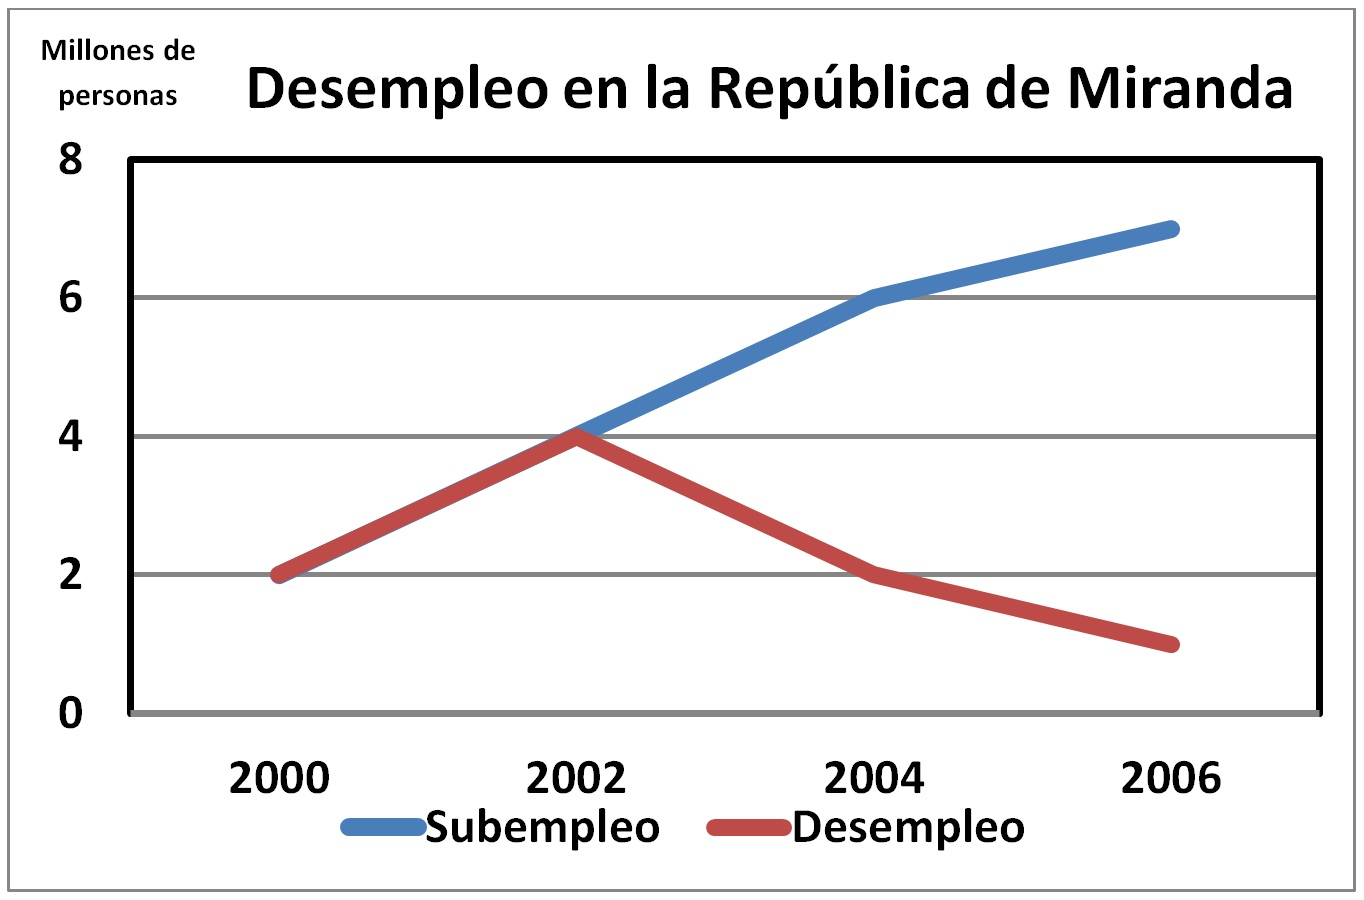
\includegraphics[width=0.45\textwidth]{sociii_img1.jpeg}

$\blacklozenge$ Se entiende por desempleo la situación de paro forzoso a la que es sometida aquella persona que teniendo las capacidades y el deseo de trabajar, no encuentra un empleo y por ende no percibe salario. \\

$\blacklozenge$ Se entiende por subempleo la situación de trabajo realizado sin suficiente regularidad o trabajo esporádico que se lleva a cabo cuando el trabajador no consigue una posición fija dentro del mercado laboral que le permita ocupar su disponibilidad temporal en un empleo estable. Dentro de esta categoría se encuentran los vendedores ambulantes y/o de economía informal.

\item De acuerdo con el gráfico 1, en la República de Miranda el subempleo:\label{sociii-23}


\begin{enumerate}[(A) ]
\item   Se toma en cuenta a partir del año 2000 registrando a dos millones de personas y para el año 2006 registraba siete millones de personas.
 \item  Se toma en cuenta a partir del año 2004 registrando a cuatro millones de personas y para el año 2006 registraba siete millones de personas.
\item Existía desde el año 2002 y registraba a dos millones de personas, pero recibía el nombre de desempleo.
\item Existía desde mucho antes de aparecer en la gráfica, pero se enmarcaba dentro de la categoría del desempleo.
\end{enumerate}
%%%%%%%%%%%%%%%%%%%%%%%%%%%%%

\item Se puede deducir que con relación a sus promesas de gobierno, el presidente Alberto Ubiria López:\label{sociii-24}


\begin{enumerate}[(A) ]
\item   Cumplió con lo prometido en tanto que la línea de desempleo disminuyó gradualmente hasta casi desaparecer por completo.
 \item  No cumplió con lo prometido debido a que nunca hubo una desaparición real del desempleo, sino una subsunción del mismo dentro de la categoría ``subempleo''.
\item Cumplió con lo prometido ya que en el 2002 recibió el país con cuatro millones de desempleados y lo entregó en el 2006 con tan sólo un millón.
\item No cumplió con lo prometido puesto que le faltó un millón de desempleados para lograr alcanzar sus metas propuestas.
\end{enumerate}
%%%%%%%%%%%%%%%%%%%%%%%%%%%%%

\item Se puede afirmar que para el 2006 la situación social y económica que atraviesa la República de Miranda es:\label{sociii-25}


\begin{enumerate}[(A)]
\item   Óptima ya que los niveles de desempleo han descendido de manera significativa.
 \item  Deficiente debido a que hay todavía un millón de personas que aún se encuentran sin trabajo.
\item Óptima puesto que de continuar la tendencia que registran las estadísticas, en menos de dos años se habría erradicado por completo el desempleo.
\item Deficiente, en tanto que se puede inferir que más de la mitad de la población se encuentra en la pobreza puesto que no existe una situación laboral estable que otorgue condiciones de trabajo y remuneración adecuados para la gran mayoría de la población. 
\end{enumerate}

%%%%%%%%%%%%%%%%%%%%%%%%%%%%%

%%%%%%%%%%%%%%%%%%%%%%%%%%%%%
\end{enumerate}
%%%%%%%%%%%%%%%%%%%%%%%%%%%%%5



\chapterimage{sociales3.jpg} % Table of contents heading image

\chapter{Literatura}\label{chap:lit1}


\subsubsection*{Marque en la hoja de respuestas la opción acertada para las preguntas \ref{lit-1}-\ref{lit-5}}

\textbf{La primera generación de cíclopes} estaba formada por los hermanos; Arges (resplandor), Brontes (trueno) y Steropes (relámpago). Estos 3 cíclopes eran, junto a los titanes y los gigantes de las cien manos, los hijos de Gaia y Urano. Se convirtieron en los herreros forjadores del Olimpo de los Dioses dada su gran aptitud para manejar el metal. También forjaron el rayo de Zeus.\\

Urano, que odiaba a sus descendientes, mantuvo a los cíclopes presos en el interior de Gaia (la diosa Tierra) hasta que fue abatido por otro de sus hijos: Cronus (un titán). Cronus temía el poder de los inmensos cíclopes así que los volvió a encerrar. Zeus rescató a los cíclopes y éstos con sus rayos ayudaron a Zeus a vencer a los Titanes.\\

\textbf{La segunda generación de cíclopes} eran los descendientes de Poseidón y no poseían la habilidad para la metalurgia que tenían sus antecesores. Se dedicaban al pastoreo en Sicilia, donde vivían bajo ninguna ley.
El más famoso de estos cíclopes es Polifemo, uno de los protagonistas de La Odisea de Homero. En el relato se cuenta que Polifemo era especialmente cruel y consiguió atrapar a Ulises y a sus doce compañeros, a los que encerró en una cueva para devorarlos vivos. Día tras día iban cayendo miembros del grupo hasta que Ulises emborrachó con vino dulce al bobo cíclope hasta dejarlo dormido. En ese momento le atacó e hirió su único ojo. Al día siguiente, con el cíclope prácticamente ciego, consiguieron escapar camuflados bajo pieles de cabras. \begin{flushright}
{\footnotesize Tomado de:\\ http://www.seresmitologicos.net/terrestres/ciclope}
\end{flushright}
\begin{enumerate}
%%%%%%%%%%%%%%%%%%%%%%%%%%%%%%%%%%

\item Según el texto anterior, el ciclope es un personaje común en la literatura \label{lit-1}


\begin{enumerate}[(A)]
\item Oriental
\item Americana
\item Griega
\item Trágica 
\end{enumerate}


%%%%%%%%%%%%%%%%%%%%%%%%%%%%%%%%%%

\item Según el texto Ulises escapa del ciclope mediante:\label{lit-2}

\begin{enumerate}[(A)]
\item La argucia.
\item La discusión. 
\item La verdad. 
\item El dialogo.
\end{enumerate}

%%%%%%%%%%%%%%%%%%%%%%%%%%%%%5

\item según el último párrafo del texto, es posible inferir que los ciclopes son seres que para Ulises representan: \label{lit-3}
\begin{enumerate}[(A)]
\item Ayuda. 
\item Oposición.
\item Guía. 
\item Proveedores.
\end{enumerate}

%%%%%%%%%%%%%%%%%%%%%%%%%%%%%
\item Según el texto, desde su origen, los ciclopes han generado\label{lit-4}
\begin{enumerate}[(A)]
\item Conflicto.
\item Alegrías.
\item Temor.
\item Guerras.
\end{enumerate}


%%%%%%%%%%%%%%%%%%%
\item a partir del texto se puede inferir que los ciclopes  son:\label{lit-5}

\begin{enumerate}[(A)]
\item Seres mitológicos que vivieron en Sicilia.
\item Seres fabulosos creados por la humanidad. 
\item Los protagonistas de la odisea
\item Los antecesores de los dioses
\end{enumerate}



\subsubsection*{Preguntas de selección múltiple con única respuesta.  Marque en la hoja de respuestas la opción acertada para las preguntas \ref{lit-6}-\ref{lit-14} a partir del siguiente texto}

\begin{center}
\textbf{LA CONCUPISCENCIA DE LOS SENTIMIENTOS\\
(Texto argumentativo)}
\end{center}


Uno de los rasgos más sobresalientes en la televisión durante los últimos años es la \textbf{\underline{exhibición impúdica}} de los sentimientos como recurso \textbf{\underline{infalible}} para el incremento de las audiencias. Se ha comprobado que la utilización \textbf{\underline{demagógica }} del dolor ajeno vende, y se ha explotado tanto, en los informativos como, en los \textit{reality shows}. En la mayor parte de los casos no se pretende analizar las situaciones de dolor, añadiendo racionalidad a la emotividad, sino embotar las sensibilidades y las conciencias anulando toda racionalidad y convirtiendo la lagrima en espectáculo.

La hipertrofia del sentimiento se corresponde con la represión de la racionalidad.  Los problemas se banalizan, se trivializan. No se pretende proyectar algo de luz sobre las situaciones dolorosas, sino aprovecharse comercialmente de ellas. Y no sólo se exhiben impúdicamente las emociones, sino que se recurre también a la humillación pública, sometiendo a concursantes y a participantes de reality shows a pruebas denigrantes.

En Estados Unidos esta tendencia alcanza límites delirantes; por ejemplo, al transmitir en vivo juicios reales sobre los casos más morbosos, o al transmitir en directo una ejecución, conseguido el \textbf{\underline{beneplácito}} del juez federal. La cadena estadounidense Court TV, que comenzó a emitir en julio de 1991, se dedicaba a retransmitir juicios reales las 24 horas del día.  El record de audiencia de la cadena lo tiene la retransmisión del juicio de Lyle y Eric Menéndez, dos hermanos de Beverly Hills que asesinaron a sus padres en el verano del 89. La prensa aireó el caso de un expolicía de Nueva York, Stanley Orlen, que atrasó su paso por el quirófano porque no quería perderse ni un solo día el juicio de los hermanos Menéndez. El lema de la emisora es elocuente. ``\textit{Si Court TV creara un poco más de adicción, sería ilegal}''

En Estado unidos unos 45 millones de personas siguen cada día los 12 \textit{talk shows}  que emiten las cadenas más populares del país. Seguramente estos espectadores esperan encontrar más confortables sus vidas al compararlas con las miserias ajenas. En marzo de 1995 un hombre mataba a otro en casa porque lo había humillado al declararle su amor ante las cámaras en uno de esos \textit{talk shows} matutinos.

En Italia, en 1994, la RAI-3 ideó y comenzó a emitir con éxito el programa: ``\textit{El, Ella y el Otro}'', emisión dedicada a parejas totas por la aparición de un tercero, amante heterosexual u homosexual de uno de ellos. Se realizaba con la presencia en el estudio de los tres interesados, que exhibían, a veces, a voz en grito, sus problemas, formulaban públicamente sus acusaciones, confesaban sus traumas… 

También las telenovelas forman parte de este resurgir de la pornografía de los sentimientos en una sociedad que, curiosamente, reprime sus sentimientos en la mayor parte de los ámbitos de la vida cotidian.  La Asociación de Telespectadores y Radioyentes hablaba de que la vida se ha dramatizado y ``ya sólo se llora ante el aparato de televisión''.

La pornografía de los sentimientos pone de manifiesto un extraordinario sentido de \textbf{\underline{exhibicionismo}} por parte de algunos ciudadanos y, además, una curiosidad morbosa cercana al voyerismo enfermizo, por parte de los espectadores. Violencia, sexo, mal gusto copan a menudo las pantallas.  No es de extrañar que en 1992 Gabe Pressman, reportero de la NBC exclamara: ``\textit{Emitimos una tonelada de basura al día}''.

Seguramente si la basura seduce, es porque remite inconscientemente al espectador a las dimensiones más oscuras de sí mismo, porque da cuerpo narcisísticamente a su fascinación por el mal,  por el dolor, por  la destrucción y la muerte, porque actúa como espejo inconsciente de las zonas más turbias del propio siquismo.


\begin{flushright}
{\footnotesize Ferres, Joan. 206. Televisión subliminal. Barcelona.  Paid\'os.}
\end{flushright}




%%%%%%%%%%%%%%%%%%%%%%%%%%%%%
\item  Las palabras exhibición impúdica corresponden respectivamente a un: \label{lit-6}

\begin{enumerate}[(A)]
\item Verbo y adverbio.
\item Sustantivo y adjetivo.
\item Artículo y preposición.
\item Conjunción y sustantivo.
\end{enumerate}

%%%%%%%%%%%%%%%%%%%%%%%%%%%%%
\item  En la frase... ``en la mayor parte de los ámbitos de la vida cotidiana'' las palabras subrayadas son respectivamente:\label{lit-7}

\begin{enumerate}[(A)]
\item Sustantivo - adjetivo.
\item Conjunción - pronombre.
\item Determinante - preposición.
\item Adverbio- verbo.
\end{enumerate}
%%%%%%%%%%%%%%%%%%%%%%%%%%%%%
\item En el primer párrafo del texto, las palabras subrayadas se pueden reemplazar respectivamente por: \label{lit-8}

\begin{enumerate}[(A)]
\item Muestra - vergonzosa - exhibicionista - habladora. 
\item Presentación - banal - charlatana - educativa- 
\item Exposición - correcta - precipitado- desahogado.
\item Manifestación - escabrosa - verdadero - populista.
\end{enumerate}
%%%%%%%%%%%%%%%%%%%%%%%%%%%%%
\item La palabra beneplácito, utilizada en el tercer párrafo, hace referencia a: \label{lit-9}


\begin{enumerate}[(A)]
\item Consentimiento.
\item Venerable.
\item Afecto.
\item Ejemplo. 
\end{enumerate}
%%%%%%%%%%%%%%%%%%%%%%%%%%%%%
\item Un sinónimo de la palabra exhibicionismo en el último párrafo, puede ser: \label{lit-10}

\begin{enumerate}[(A)]
\item Emboscada.
\item Exteriorización.
\item Peregrinación.
\item Exclusivismo. 
\end{enumerate}
%%%%%%%%%%%%%%%%%%%%%%%%%%%%%
\item El autor califica de voyeristas a los televidentes porque: \label{lit-11}


\begin{enumerate}[(A)]
\item Sienten satisfacción personal al observar las emociones y sentimientos más íntimos en personas de la televisión.
\item Manifiestan un tipo de parafilia relativa al disfrute ocasionado al observar actos íntimos.
\item Demuestran una evidente preferencia por los viajes en lugar de ver televisión.
\item Él siente un gran desprecio por los personajes de la televisión y por los televidentes.
\end{enumerate}
%%%%%%%%%%%%%%%%%%%%%%%%%%%%%
\item Para el autor, la televisión cautiva a los espectadores en gran medida. Porque: \label{lit-12}

\begin{enumerate}[(A)]
\item Es un medio de comunicación masivo al cual todo el mundo tiene acceso.
\item La televisión en Estados Unidos es de bastante contenido y bien hecha.
\item La televisión y el Internet atrofian el cerebro de los jóvenes.
\item Sienten más confortables sus vidas al compararlas con las tragedias ajenas. 
\end{enumerate}
%%%%%%%%%%%%%%%%%%%%%%%%%%%%%
\item A partir del texto, se puede inferir, que la posición del autor frente a la televisión es: \label{lit-13}

\begin{enumerate}[(A)]
\item Aprobatoria.
\item Crítica.
\item Desmedida.
\item Legal.
\end{enumerate}
%%%%%%%%%%%%%%%%%%%%%%%%%%%%%
\item En el texto, Gabe Pressman afirma: ``Emitimos una tonelada de basura al día''. Dicha expresión significa que: \label{lit-14}


\begin{enumerate}[(A)]
\item La televisión está produciendo programas de alta calidad y contenido.
\item Las programadoras desconocen los planes de reciclaje.
\item La televisión está produciendo programas que carecen de alta calidad y contenido.
\item La televisión debe apoyar el programa de ``Basura Cero''.
\end{enumerate}



%%%%%%%%%%%%%%%%%%%%%%%%%%%%%%%%%%%%%5

\subsubsection*{Lea los siguientes párrafos y responda las preguntas \ref{lit-15}-\ref{lit-20}}

\begin{center}
\textbf{¿CUÁL SERÁ EL FIN DE LA TIERRA?	}
\end{center}

 
En estas condiciones, también la Tierra se iría enfriando lentamente. El agua se congelaría y las regiones polares serían cada vez más extensas. En último término, ni siquiera las regiones ecuatoriales tendrían suficiente calor para mantener la vida.  El océano entero se congelaría en un bloque macizo de hielo, e incluso el aire se licuaría primero y se congelaría luego. Durante billones de años, esta Tierra gélida (y los demás planetas) seguiría girando alrededor del difunto Sol. Pero aun en esas condiciones, la Tierra, como planeta, seguiría existiendo.


 En tales condiciones, es probable que la Tierra se convierta en un ascua y luego se vaporice. En ese momento, la Tierra, como cuerpo planetario sólido, acabará sus días. Pero no os preocupéis demasiado: échale todavía ocho mil millones de años.


Hasta los años treinta, parecía evidente que el Sol, como cualquier otro cuerpo caliente, tenía que acabar enfriándose. Vertía y vertía energía al espacio, por lo cual este inmenso torrente tendría que disminuir y reducirse poco a poco a un simple chorrito. El Sol se haría naranja, luego rojo, iría apagándose cada vez más y, finalmente, se apagaría.	


 Sin embargo, durante la década de los treinta, los científicos nucleares empezaron a calcular por primera vez las reacciones nucleares que tienen lugar en el interior del Sol y otras estrellas. Y hallaron que, aunque el Sol tiene que acabar por enfriarse, habrá períodos de fuerte calentamiento antes de ese fin. Una vez consumida la mayor parte del combustible básico, que es el hidrógeno, empezarán a desarrollarse otras reacciones nucleares que calentarán el Sol y harán que se expanda enormemente. Aunque emitirá una cantidad mayor de calor, a cada porción de su ahora vastísima superficie le tocará una fracción mucho más pequeña de ese calor y será, por tanto, más fría.  El Sol se convertirá en una masa gigante roja. 
Isaac Asimov, Cien preguntas básicas sobre la ciencia.  

\begin{flushright}
{\footnotesize Tomado de:\\
Isaac Asimov, Cien preguntas básicas sobre la ciencia.\\
 http://www.xtea.cat/~jgenover/ordtexto3.htm}
\end{flushright}



%%%%%%%%%%%%%%%%%%%%%%%%%%%%%%%%555
\item La opción que corresponde al orden lógico del texto es: \label{lit-15}


Final del formulario

\begin{enumerate}[(A)]
\item  A - B - C - D 
\item  C - A - D - B
\item  C - D - B - A
\item  B - C -  D -  A 
\end{enumerate}
%%%%%%%%%%%%%%%%%%%%%%%%%%%%%%%%555
\item La idea principal y la conclusión del texto se encuentran respectivamente en los párrafos: \label{lit-16}


\begin{enumerate}[(A)]
\item  A - D
\item  B - C 
\item  A - C
\item  C - B 
\end{enumerate}
%%%%%%%%%%%%%%%%%%%%%%%%%%%%%%%%555
\item  Según su estructura el texto completo puede ser clasificado como:\label{lit-17}


\begin{enumerate}[(A)]
\item  Deductivo porque presenta una idea general y cierra con una idea particular.
\item  Inductivo porque parte de una idea especifica.
\item  Deductivo-inductivo porque la idea general se desarrolla con ideas secundarias y cierra con una conclusión.
\item  Inductivo-deductivo la idea principal está en la mitad del texto, y las ideas de la conclusión se deben desarrollar.
\end{enumerate}
%%%%%%%%%%%%%%%%%%%%%%%%%%%%%%%%555
\item  Según su finalidad el párrafo A del texto anterior se puede clasificar como:\label{lit-18}

\begin{enumerate}[(A)]
\item  Expositivo-Argumentativo porque presenta una idea y la sustenta con argumentos.
\item   Narrativo-Argumentativo porque presenta una idea y la sustenta con argumentos que relatan una historia. 
\item  Descriptivo- Expositivo porque presenta una idea y las características de un hecho, objeto o fenómeno.
\item  Argumentativo-Descriptivo porque presenta una idea y las características de un hecho, objeto o fenómeno.
\end{enumerate}
%%%%%%%%%%%%%%%%%%%%%%%%%%%%%%%%555
\item Según su estructura el párrafo D del texto anterior se puede clasificar como:\label{lit-19}

\begin{enumerate}[(A)]
\item  Conclusión porque cierra las ideas.
\item  Introducción porque contiene la idea principal.
\item  Enlace porque conecta información presentada anteriormente.
\item  Desarrollo porque presenta argumentos que sustentan la idea principal.
\end{enumerate}
%%%%%%%%%%%%%%%%%%%%%%%%%%%%%%%%555
\item  La expresión Sin embargo corresponde a un conector formado por una conjunción de tipo: \label{lit-20}


\begin{enumerate}[(A)]
\item  Aditivo.
\item  Temporal.
\item  Locativo.
\item  Adversativo.
\end{enumerate}

\subsubsection*{\textbf{PREGUNTAS ABIERTAS}
En relación con el siguiente texto responda las preguntas \ref{lit-21}-\ref{lit-25}}

A manera de introducción se hace necesario definir la literatura desde su dimensión filosófica ya que ésta valida el carácter epistemológico de la misma. La literatura es una episteme porque es una forma de conocer el mundo y la manera como nos relacionamos con él. La obra literaria permite reflexionar sobre la vida, el ser, la sociedad, la historia, la cultura, e incluso sobre el conflicto mismo de ser humano. Sin embargo, el objeto de conocimiento de la literatura no se enmarca dentro de las ciencias positivas,  caracterizadas por su racionalidad y empirismo, así como tampoco responde a las lógicas del mundo cotidiano. El objeto de conocimiento de la literatura permite construir un saber desde la sensibilidad  porque el elemento central  de su existir es la correlación entre el hombre y su mundo de vida, es decir desde la fenomenología.


 La fenomenología, tal como la define Gadamer en su texto “Verdad y Método” se constituye como la ciencia que orienta  y valida el saber del hombre sobre sí mismo en el ámbito de la experiencia, esto permite concebir la literatura como  recurso que permite al hombre construir un saber de si en el mundo de la vida. 
 
 
Sartre se basa en la fenomenología para definir la literatura porque la concibe como una cuestión esencial de la cultura en tanto es un arte y como tal se convierte en un componente fundamental de la condición del ser. En ese sentido la literatura según Sartre se transforma en un símbolo del ser al darle sentido a su proceso existencial histórico y cultural a través del lenguaje.


 Para sustentar la definición de Jean-Paul Sartre en el presente documento se sintetizan tres premisas fundamentales que se inter-relacionan y construyen mutuamente alrededor de la literatura, la primera es la escritura como arte, la segunda es la escritura como emancipación, y la tercera la dialéctica entre escritor, lector y obra. Además, se establece la relación entre la literatura y la labor docente.
 
 
En primer lugar, la escritura es entendida como arte porque el escritor pinta el mundo con palabras, en la poética se concibe el lenguaje como una metáfora del mundo que permite la metamorfosis de las emociones y sentimientos en las palabras, al punto que es imposible para el escritor diferenciar los unos de las otras. El hombre se construye a través del lenguaje porque, como dice Chomsky, estamos hechos desde y para el lenguaje. Dependiendo del uso que el escritor le dé al lenguaje se le reconocerá como prosista o como poeta. El primero se rodea de las palabras y las concibe como un espejo del mundo y por lo tanto Sartre lo niega como parte de la literatura. Dado que para él la literatura no es un marco de referencia y mucho menos existe para hacer una copia de las experiencias es imposible establecer una realidad universal.


Por otro lado, para el poeta las palabras son ``el medio para atrapar la realidad huidiza''; por lo tanto, dan cuenta de la forma que el hombre percibe el mundo. El poeta tiene el poder de crear mundos, es decir, la poesía le da la posibilidad de crear un conjunto infinito de posibilidades de sentido. Y entonces aparece la cuestión ¿cuál es el compromiso del escritor?  Al respecto, Sartre responde que el prosista es más comprometido que el poeta porque tiene la posibilidad de servirse de las palabras para crear conciencia. El prosista comprometido debe revelar el mundo y provocar indignación; de este modo, logrará establecer una relación con el lector y llegar a un acuerdo que les permitirá transformar la realidad. Por su parte, el poeta comprometido debe trascender su realidad histórica y escribir por y para la libertad.


Ese compromiso con la libertad humana define la escritura como emancipación al reflexionar el rol del escritor y del lector desde el ámbito social. En el cual se requiere de la negociación entre el uno y el otro. El poeta crea para revelar y producir nuevos mundos bajo sus propias reglas, esto significa que dada su función social de `guardián de los valores ideales', escribe para la libertad, ésa es su única manera de existir, para Sartre `el poeta no es libre por decisión es libre de hecho'. Sin embargo, para que ese ideal de libertad sea alcanzado se requiere de la relación dialógica y simbiótica entre el escritor, la obra y el lector. Esto quiere decir que el escritor necesita de un lector comprometido, dispuesto a construir el significado de la obra que él proyecta. La libertad del lector le permite descubrir lo bello que tiene el mundo desde su subjetividad. Entre tanto, La obra por sí misma no existe, pasa a ser un ente  dependiente de `su' lector-creador porque gracias a él la obra pasa de existir a ser. Así pues, el escritor aprende a confiar en la capacidad creadora del lector apelando a su libertad y el lector cumple su función y re-crea el mundo que le es revelado a través de la experiencia estética. 


La relación dialéctica del triado escritor, obra, lector nos lleva a la tercera premisa la cual invita a relacionar estos tres elementos dentro de un contexto histórico para lograr una sociedad consciente de sí misma. Desde  un punto de vista fenomenológico esa relación puede ser descrita de la siguiente manera. El escritor se erige como mediador y revelador del conflicto entre la organización social  y el lector, luego es el lector quien establece la esencia de la obra, un lector ideal comprometido con la re-creación de la obra y con la toma de conciencia sobre el uso de su libertad como fin último será capaz de dar sentido a la existencia humana desde la obra.


 Así pues, la obra se establece como un ente inacabado, fuente de conocimiento, que permite relacionar experiencias, comunicar deseos, liberar lo humano en tanto se construye en cada lector y trasciende a una realidad metafísica. 

\item ¿Qué es literatura? \label{lit-21}

\item ¿Por qué la literatura trasciende su tiempo y aún no ha llegado a su fin?\label{lit-22}
	
\item ¿Cuál es la relación entre filosofía y literatura?\label{lit-23}

\item ¿Cuál debe ser el compromiso del autor y de lector?\label{lit-24}

\item ¿La literatura tiene carácter de conocimiento?\label{lit-25}
	

%%%%%%%%%%%%%%%%%%%%%%%%%%%%%
\end{enumerate}
%%%%%%%%%%%%%%%%%%%%%%%%%%%%%5





%%%%%%%%%%%%%%%%%%%%%%%%%%%%%%%%%%%%%%%%%%%%%%%%%%
%%%%%%%%%%%%     Ciencias Quimica %%%%%%%%%%%%%%
%%%%%%%%%%%%%%%%%%%%%%%%%%%%%%%%%%%%%%%%%%%%%%%%%%

\chapterimage{quim3v.jpg} % Table of contents heading image

\chapter{Qu\'{i}mica I}\label{chap:quim1}

\begin{enumerate}
%%%%%%%%%
\item Para reconocer el estado en que esta la materia, su ordenamiento molecular está definido por la presión y temperatura a que este sometido para alejar o separar sus moléculas, llevando a ésta sustancia al estado sólido, líquido, gaseoso o plasma. El estado en el que se encuentra una sustancia a temperatura de -15$^o$C si su punto de ebullición es a 15$^o$C y de fusión es -12$^o$C es: \label{mon-1}


\begin{enumerate}[(A)]
\item Gaseoso porque sus moléculas se han separado.
\item Líquido porque sus moléculas experimentan cierto debilitamiento de sus enlaces. 
\item Líquido porque sus moléculas se han separado. 
\item Sólido porque sus moléculas están fuertemente enlazadas. 
\end{enumerate}

%%%%%%%%%%%
\item El diagrama de configuración electrónica presenta (figura \ref{fig:mon-2}) para cada nivel los subniveles y los electrones que les corresponde, como se muestra a continuación: \label{mon-2}

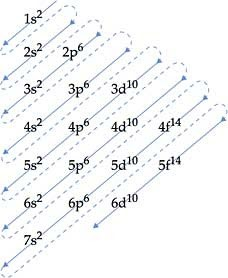
\includegraphics[width=0.35\textwidth]{imagen_0.jpg}
%\centering\captionof{figure}{Pregunta \ref{mon-2}}\label{fig:mon-2}
\justifying

Siguiendo ese diagrama para representar el siguiente átomo la configuración electrónica es:

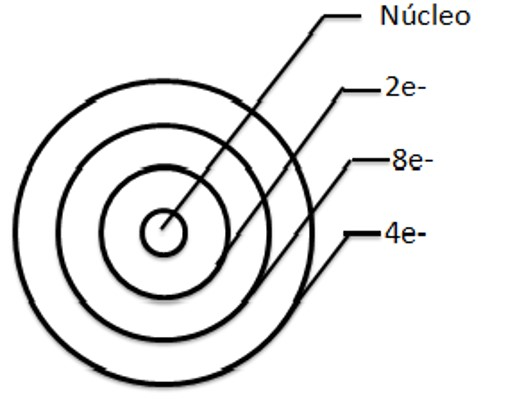
\includegraphics[width=0.45\textwidth]{imagen_1.jpg}
%\centering\captionof{figure}{Pregunta \ref{mon-2}}\label{fig:mon-2-2}
\justifying

\begin{enumerate}[(A)]
\item 1s$^2$ 2s$^2$ 2p$^6$ 3s$^2$ 3p$^4$
\item 1s$^2$ 2s$^2$ 3p$^2$ 2p$^6$ 3p$^4$
\item 1s$^2$ 2s$^2$ 2p$^6$ 3s$^2$ 3p$^2$
\item 1s$^2$ 2s$^2$ 3p$^2$ 2p$^6$ 4s$^2$
\end{enumerate}

%%%%%%%%%%%%%%
\item La estructura de Lewis es una representación de los electrones de valencia implicados en el enlace entre dos o más átomos. De acuerdo con la siguiente tabla, la estructura de Lewis que representa la molécula CO$_2$ es:\label{mon-3}


\begin{center}
\begin{tabular}{|ccc|}
\hline 
Características & C & O \\  
\hline 
Numero de e$^-$ & 6 & 8 \\ 
Numero de Protones & 6 & 8 \\ 
Numero de Neutrones & 6 & 8 \\ 
e$^-$ de valencia & 4 & 6 \\ 
\hline 
\end{tabular} 
\end{center}

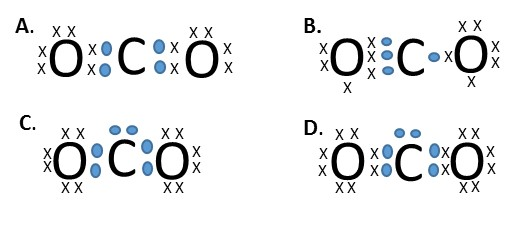
\includegraphics[width=0.45\textwidth]{imagen_2.jpg}
%\centering\captionof{figure}{Pregunta \ref{mon-3}}\label{fig:mon-3}
\justifying


%%%%%%%%%%%%%%%%%
\item La electronegatividad es una medida de la fuerza de atracción que ejerce un átomo sobre los electrones de otro y la diferencia entre las electronegatividades determina el tipo de enlace.  
En la siguiente tabla se presenta la electronegatividad de algunos elementos, por lo que el compuesto que posiblemente forme un enlace iónico es: \label{mon-4}


\begin{center}
\begin{tabular}{|ccccc|}
\hline 
Elemento & X & J & Y & L \\ 
\hline 
Electronegatividad & 4 & 1.5 & 0.9 & 1.6 \\ 
\hline 
\end{tabular} 
\end{center}
\begin{enumerate}[(A)]
\item YL
\item JL
\item YJ
\item YX
\end{enumerate}

%%%%%%%%%%%%%%%
\item Los iones, son especies químicas que han ganado o cedido electrones convirtiendo se en aniones o cationes, los aniones al ``ganar'' electrones queda con carga neta negativa y los cationes al ``perder'' electrones quedan con una carga neta positiva. El ión Cu$^{+2}$ cuenta con: \label{mon-5}

\begin{enumerate}[(A)]
\item 2 protones más que el átomo de cobre neutro.
\item 2 protones menos que el átomo de cobre neutro.
\item 2 electrones más que el átomo de cobre neutro.
\item 2 electrones menos que el átomo de cobre neutro.
\end{enumerate}

%%%%%%%%%%%%%%%%
\item Existen fuerzas al interior de los átomos de una molécula que se llaman \textbf{intramoleculares} y restando sus electronegatividades se puede conocer si se trata de un enlace iónico, covalente o metálico. Las fuerzas \textbf{intermoleculares} se refieren a atracción de moléculas para formar un estado de la materia y pueden ser dipolo-dipolo, ion-dipolo fuerzas de London o puentes de hidrógeno. Según el siguiente esquema La intensidad de fuerzas intermoleculares de los 3 estados de la materia organizada de menor a mayor es:\label{mon-6}

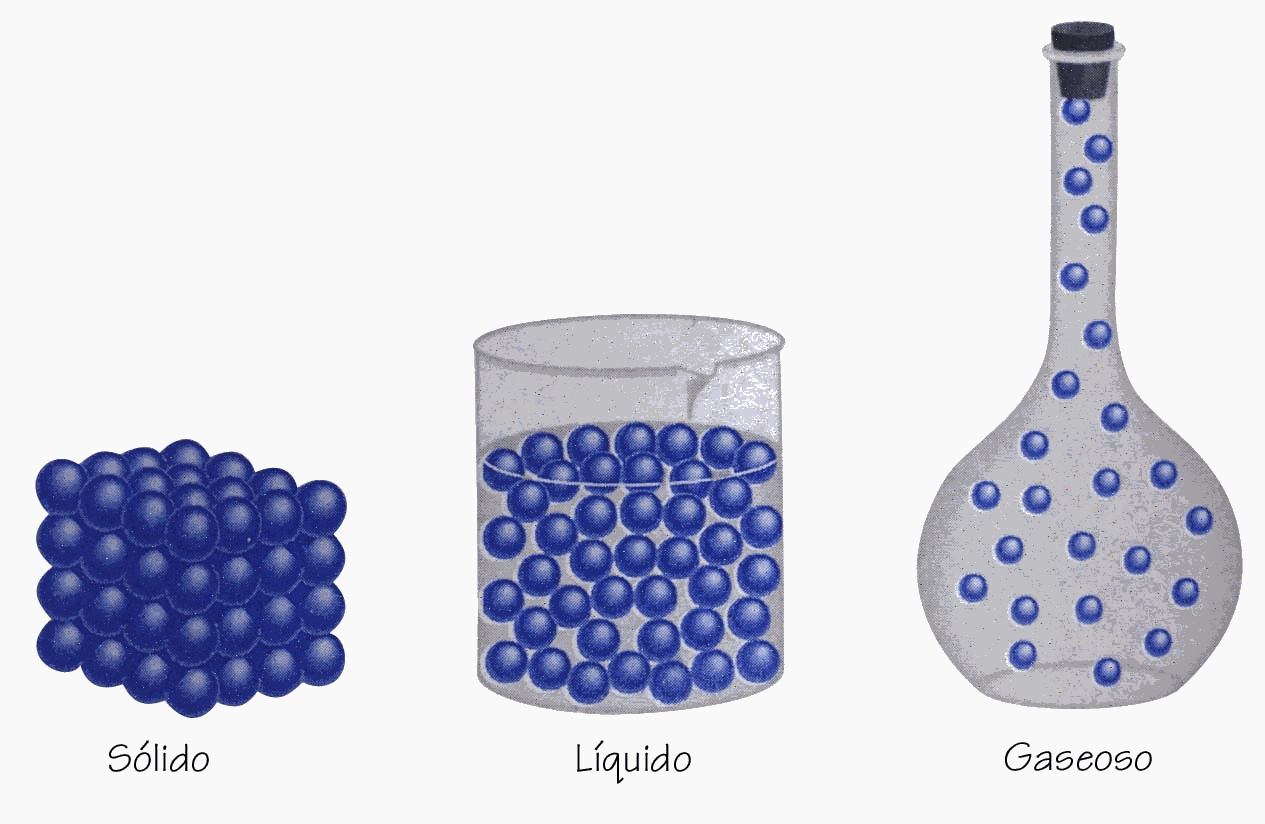
\includegraphics[width=0.45\textwidth]{imagen_4.jpg}
%\centering\captionof{figure}{Pregunta \ref{mon-3}}\label{fig:mon-6}
\justifying

\begin{enumerate}[(A)]
\item Líquido, sólido y gaseoso.
\item Gaseoso, líquido y sólido.
\item Líquido, gaseoso y sólido.
\item Sólido, líquido y gaseoso.
\end{enumerate}


%%%%%%%%%%%%%%%%
\item Con los diagramas de atómicos se identifican electrones de valencia, grupo, periodo, número atómico y por consiguiente número de electrones y protones. Además se usan las siguientes ecuaciones: \label{mon-7}

\begin{itemize}
\item Número de protones (\#p$^+$) = Número atómico (Z)
\item \#p$^+$ = Número de electrones (\#e$^-$)
\item \#neutrones = Masa atómica (A) - \#p$^+$
\end{itemize}

De acuerdo a los siguientes diagramas se presentan a continuación, una serie de afirmaciones, de las cuales NO son válidas:

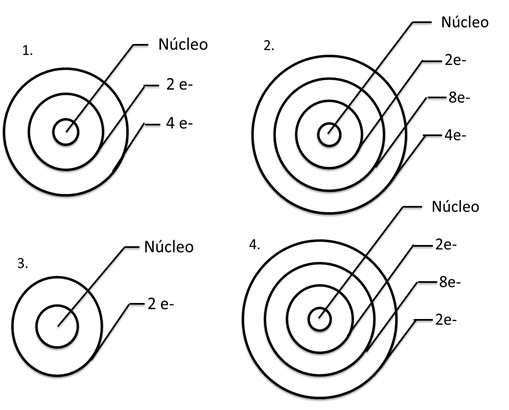
\includegraphics[width=0.45\textwidth]{imagen_5.jpg}
%\centering\captionof{figure}{Pregunta \ref{mon-3}}\label{fig:mon-7}
\justifying

\begin{enumerate}[I]
\item 1. Los diagramas 2 y 4 muestran átomos del periodo 3 
\item El diagrama 1 presenta \#e$^-$ de valencia: 4,  \#p$^+$: 6,  Z: 6, periodo:4
\item El diagrama 4 presenta \#e$^-$ de valencia: 8,  \#p$^+$: 12,  Z: 6, periodo:2
\item El diagrama 3 presenta \#e$^-$ de valencia: 2,  \#p$^+$: 2,  Z: 2, periodo:1
\end{enumerate}

\begin{enumerate}[(A)]
\item I
\item II y IV
\item I y II
\item III
\end{enumerate}


%%%%%%%%%%%%%%%%%%%%%%%%%%%
\item Una mezcla homogénea presenta una sola fase y una mezcla heterogénea dos o más fases visibles. Si se trata de una mezcla homogénea puede ser una solución cuando está compuesta de moléculas o compuestos diferentes o puede ser una sustancia pura si se compone de un solo tipo de molécula o compuesto.   El aire es una mezcla de varios gases, tales como O$_2$, N$_2$, CO, CO$_2$, CH$_4$, entre otros, por lo tanto el aire es: \label{mon-8}

\begin{enumerate}[(A)]
\item Una mezcla homogénea y sustancia pura.
\item Una mezcla heterogénea.
\item Una mezcla homogénea y solución.
\item Una mezcla heterogénea y sustancia pura. 
\end{enumerate}

%%%%%%%%%%%%%%%%%%%%%%%%%
\item La separación de una mezcla se realiza a partir de diferentes técnicas, entre éstas se encuentran: \label{mon-9}

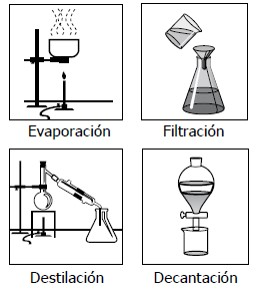
\includegraphics[width=0.45\textwidth]{imagen_6.jpg}
%\centering\captionof{figure}{Pregunta \ref{mon-3}}\label{fig:mon-7}

De éstas, la mejor técnica para desalinizar agua de mar es:
\begin{enumerate}[(A)]
\item Destilación y filtración
\item Evaporación
\item Destilación 
\item Decantación
\end{enumerate}

%%%%%%%%%%%%%%%%%%%%%%%%%%%%%%%%%%%%%%%%%%%

\item Con la destilación se separan los componentes de petróleo utilizados en las diferentes industrias a nivel mundial. En la siguiente figura se presentan los puntos de ebullición de éstos componentes, por lo que el orden en que se obtienen algunos de ellos en la destilación es:\label{mon-10}

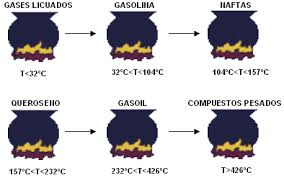
\includegraphics[width=0.45\textwidth]{imagen_7.jpg}
%\centering\captionof{figure}{Pregunta \ref{mon-3}}\label{fig:mon-7}

\begin{enumerate}[(A)]
\item Compuestos pesados, queroseno y gasolina.
\item Queroseno, gasolina y compuestos pesados
\item Gasolina, queroseno y compuestos pesados
\item Compuestos pesados, gasolina y queroseno 
\end{enumerate}

%%%%%%%%%%%%%%%%%%%%%%%%%%%%%%%%%%%%%%%%%%%%%%%
\item El astato At, es un no metal que trabaja con estados de oxidación 1,3, 5 y 7. Los ácidos se forman por la reacción de un óxido ácido y agua y las bases se forman por la reacción de un óxido básico y agua. La reacción para el ácido astático es: \label{mon-11}


\begin{enumerate}[(A)]
\item As$^{+3}$ + O$^{-2}$ $\;$ As$_2$O$_3$ + H$_2$O $\;$ As(OH)$_3$
\item As$^{+5}$ + O$^{-2}$ $\;$     As$_2$O$_5$ + H$_2$O	 $\;$  As(OH)$_5$ 
\item As$^{+5}$ + O$^{-2}$ $\;$     As$_2$O$_5$ + H$_2$O	 $\;$  H$_2$As$_2$O$_6$
\item As$^{+7}$ + O$^{-2}$ $\;$     As$_2$O$_7$ + H$_2$O	   H$_2$As$_2$O$_8$
\end{enumerate}

%%%%%%%%%%%%%%%%%%%%%%%%%%%%%%%%
\item Dependiendo de la presión y temperatura a la que se someta un material, se puede construir su diagrama de fases para observar los distintos estados de agregación. En la siguiente figura, se presentan los cambios de estado. La relación con el diagrama de fases de una sustancia desconocida que pasa del punto 1 al punto 2, experimenta los siguientes cambios de estado: \label{mon-12}

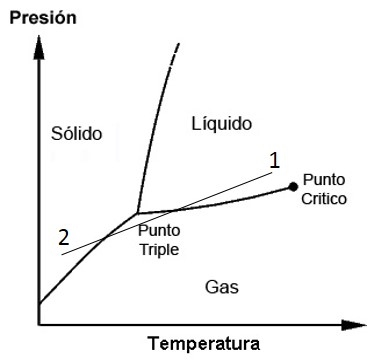
\includegraphics[width=0.45\textwidth]{imagen_9.jpg}
%\centering\captionof{figure}{Pregunta \ref{mon-3}}\label{fig:mon-7}
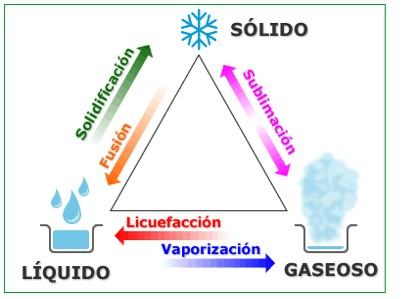
\includegraphics[width=0.45\textwidth]{imagen_8.jpg}
%\centering\captionof{figure}{Pregunta \ref{mon-3}}\label{fig:mon-7}

\begin{enumerate}[(A)]
\item Vaporización y solidificación
\item Vaporización y sublimación
\item Sublimación y licuefacción
\item Sublimación y fusión
\end{enumerate}

%%%%%%%%%%%%%%%%%%%%%%%%%%%%%%%%%%%%%%%%%%
\item La solubilidad se define como la cantidad máxima de soluto que puede disolverse en un disolvente a una presión y temperatura dada. En la siguiente gráfica se presenta la solubilidad de diversas sustancias en 100$g$ de agua y su variación con el cambio la temperatura. \label{mon-13}


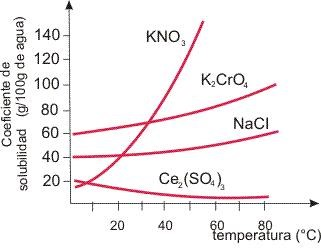
\includegraphics[width=0.4\textwidth]{imagen_10.jpg}
%\centering\captionof{figure}{Pregunta \ref{mon-3}}\label{fig:mon-7}
\begin{enumerate}[(A)]
\item Cloruro de sodio y sulfato de cesio.
\item Nitrato de potasio y dicromato de potasio.
\item Cloruro de sodio y dicromato de potasio.
\item Nitrato de potasio.
\end{enumerate}


%%%%%%%%%%%%%%%%%%%%%%%%%%%%%%%%%%%%%%%%%%
\item El magnesio es un elemento que el organismo necesita para funcionar correctamente. Su óxido es usado como antiácido, laxante o suplemento alimenticio. Se obtiene gracias a la acción del oxígeno sobre el metal con la siguiente reacción: \label{mon-14}

\begin{center}
\begin{tabular}{|cc|}
\hline 
Sustancia & Masa molar (g/mol) \\
\hline 
Mg & 24\\
O & 16 \\
\hline 
\end{tabular} 
\end{center}
\begin{equation*}
2Mg + O_2   \qquad \qquad        2 MgO   
\end{equation*}

Si existe suficiente cantidad de reactivos, para producir 10 g de MgO se necesita:

\begin{enumerate}[(A)]
\item 2.5 mol de Mg y 1,25 mol de O$_2$
\item 0.25 mol de Mg y 0,25 mol de O$_2$
\item 0.25 mol de Mg y 0,125 mol de O$_2$
\item 2.5 mol de Mg y 2.5 mol de O$_2$
\end{enumerate}

%%%%%%%%%%%%%%%%%%%%%%%%%%%%%%%%%%%%%%%%%%
\item La contaminación ambiental produce óxidos que al reaccionar con el agua de la atmosfera produce diversos ácidos, que al condensarse producen la lluvia ácida. El óxido de azufre (VI) produce ácido sulfúrico (H$_2$SO$_4$), el dióxido de carbono produce ácido carbónico (H$_2$CO$_3$). Si en una zona geográfica específica la cantidad de SO$_3$ producido genera 120 mL del ácido por cada 300mL de solución y un 56\% de concentración volumen-volumen de ácido carbónico, el ácido que más daño causa al caer por estar más concentrado es: \label{mon-15}

\begin{enumerate}[(A)]
\item El H$_2$SO$_4$ debido a que tiene un volumen mayor al de la concentración de H$_2$CO$_3$.
\item El H$_2$CO$_3$ debido a que su solución tiene un volumen menor y está más concentrado que el H$_2$SO$_4$.
\item El H$_2$SO$_4$ debido a que su concentración es mayor a la del H$_2$CO$_3$.
\item El H$_2$CO$_3$ debido a que su concentración del 56\% en comparación con el 40\% de H$_2$SO$_4$.
\end{enumerate}


%%%%%%%%%%%%%%%%%%%%%%%%%%%%%%%%%%%%%%%%%%
\item Un mol se define como la cantidad de sustancia que contiene $6,023 \times 10^{23} $ partículas, ya sea de un elemento o de un compuesto. Fue el italiano Amadeo Avogadro quien descubrió que volúmenes iguales de diferentes gases, bajo las mismas condiciones de temperatura y presión contenían igual número de moléculas. Según lo anterior, dos recipientes de igual capacidad contienen respectivamente 2 moles de N$_2$ y 2 moles de H$_2$, por lo que es válido afirmar que: \label{mon-16}

\begin{enumerate}[(A)]
\item La masa en los dos recipientes es igual.
\item  El volumen de los dos gases es igual.
\item  El número de moléculas de O$_2$ es mayor que el de N$_2$.
\item Los dos recipientes contiene igual número de moléculas.
\end{enumerate}


%%%%%%%%%%%%%%%%%%%%%%%%%%%%%%%%%%%%%%%%%%
\item La reacción F+ C  $\Longrightarrow$  Z + H se hace por duplicado y se reportan en la siguiente tabla las masas de reactivos y productos. \label{mon-17}

\begin{center}
\begin{tabular}{|ccccc|}
\hline 
Experimento & \multicolumn{2}{c}{Masa} & \multicolumn{2}{c|}{Masa}\\
 & \multicolumn{2}{c}{reactivos} & \multicolumn{2}{c|}{productos}\\ 
\hline 
 & F & C & Z & H \\ 

1 & 5 & 10 & 13 & 2 \\ 

2 & 10 & 20 & 8 & 22 \\ 
\hline 
\end{tabular}  

Según los datos reportados en la tabla es válido afirmar que se cumple la ley de la conservación de la materia porque:

\end{center}
\begin{enumerate}[(A)]
\item El número de sustancias reaccionantes es igual al número de sustancias obtenidas.
\item La masa de los productos es menor que la masa de los reactivos. 
\item La masa de los productos es igual a la masa de los reactivos.
\item El número de moles de los productos es igual al número de moles de los productos.
\end{enumerate}

%%%%%%%%%%%%%%%%%%%%%%%%%%%%%%%%%%%%%%%%%%
\item A 20$^o$C, un recipiente contiene un gas. En la siguiente figura se muestra el volumen del gas a diferentes presiones.\label{mon-18}


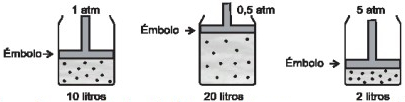
\includegraphics[width=0.45\textwidth]{imagen_11.jpg}
%\centering\captionof{figure}{Pregunta \ref{mon-3}}\label{fig:mon-7}

La grafica que mejor describe la variación del volumen cuando cambia la presión es



\begin{enumerate}[(A)]
\item 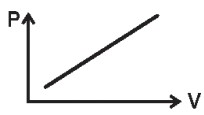
\includegraphics[width=0.4\textwidth]{imagen_12.jpg}
\item 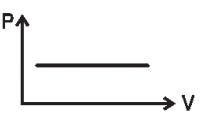
\includegraphics[width=0.4\textwidth]{imagen_13.jpg}
\item 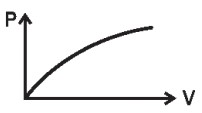
\includegraphics[width=0.4\textwidth]{imagen_14.jpg}
\item 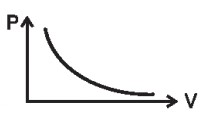
\includegraphics[width=0.4\textwidth]{imagen_15.jpg}
\end{enumerate}


%%%%%%%%%%%%%%%%%%%%%%%%%%%%%%%%%%%%%%%%%%
\item María agrega 3 cm3 de un gas a un pistón (ver figura \ref{fig:mon-19-1}). Posteriormente aumenta su temperatura sin afectar su presión (ver figura \ref{fig:mon-19-2}) \label{mon-19}

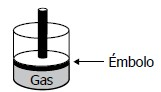
\includegraphics[width=0.4\textwidth]{imagen_16.jpg}
\captionof{figure}{}\label{fig:mon-19-1}
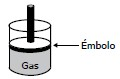
\includegraphics[width=0.4\textwidth]{imagen_17.jpg}
\captionof{figure}{}\label{fig:mon-19-2}

Desea conocer si el volumen aumentó o disminuyo de manera directa o inversamente proporcional al aumentar la temperatura. \hrulefill\\
\_\hrulefill\\
\_\hrulefill\\
\_\hrulefill.

%%%%%%%%%%%%%%%%%%%%%%%%%%%%%%%%%%%%%%%%%%
\item En el laboratorio se realizó el procedimiento que se describe en el diagrama, para identificar los cationes plata Ag$^+$, plomo Pb$^{2+}$ y mercurio Hg$^{+}$ en una muestra problema \label{mon-20}


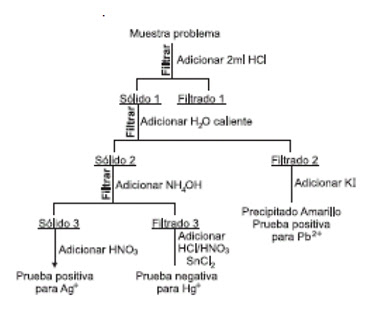
\includegraphics[width=0.45\textwidth]{imagen_18.jpg}
%\centering\captionof{figure}{Pregunta \ref{mon-3}}\label{fig:mon-7}

Durante el procedimiento se realizó una prueba de pH para cada uno de los filtrados arrojando los siguientes resultados:

\begin{enumerate}[(A)]
\item Filtrado 1 es ácido, 2 es neutro y 3 es ácido.
\item Filtrado 1 es neutro, 2 es básico y 3 es ácido. 
\item Filtrado 1 es ácido, 2 es neutro y 3 es básico.
\item Filtrado 1 es básico, 2 es ácido y 3 es neutro.
\end{enumerate}

%%%%%%%%%%%%%%%%%%%%%%%%%%%%%%%%%%%%%%%%%%
\item Durante la respiración celular se genera CO2 que se libera al torrente sanguíneo, donde puede reaccionar con agua para formar ácido carbónico, H2CO3 y contribuir, consecuentemente, al equilibrio acido - base; el proceso se ilustra mediante la siguiente serie de ecuaciones \label{mon-21}

\begin{enumerate}[(1)]
\item CO$_{2 (g)}$ + H$_2$O$_{(l)}$ $\qquad $ H$_2$CO$_{3 (ac)}$
\item   H$_2$CO$_{3 (ac)}$     $\qquad $ HCO$_{3 (ac)}^-$ + H$_{(ac)^+}$
\item  HCO$_{3 (ac)}^-$       $\qquad\ $  CO$_{3(ac)}^=$ + H$^{+}_{(ac)}$
\end{enumerate}

La siguiente tabla presenta algunas teorías del concepto ácido base.
\begin{tabular}{|p{.95in}p{2.2in}|}
\hline 
Autores & Teoría\\
\hline 
J.N Bronsted \& & \textit{Ácido}: Molécula o ion capaz de donar un protón (ion H$^{+}$) a otra sustancia. \\
T.M Lowry &\textit{Base}: Molécula o ion capaz de captar un protón (ion H$^{+}$). \\
\hline 
Gilbert & \textit{Ácido}: Molécula o ion capaz de aceptar un par de electrones libres para formar un enlace covalente. \\
\hline 
Newton  Lewis & \textit{Base}: Molécula o ion capaz de donar un par de electrones libres para formar un enlace covalente.\\
\hline 
\end{tabular} 


\begin{enumerate}[(A)]
\item 2, como una base porque tiene átomos de H en su estructura.
\item  3, como una base porque dona al medio un par de electrones libres.
\item  3, como un ácido porque libera al medio protones (iones H$^{+}$).
\item 2, como un ácido porque puede aceptar protones (iones H$^{+}$) del medio.
\end{enumerate}


%%%%%%%%%%%%%%%%%%%%%%%%%%%%%%%%%%%%%%%%%%
\item Un sistema se considera en equilibrio cuando la velocidad de formación de productos coincide con la velocidad de descomposición de éstos. Según Louis Le Chatelier, al cambiar las condiciones del equilibrio, tales como la concentración de reactivos o productos, la reacción se desplazará en la dirección que tienda a restablecer el equilibrio. Un ejemplo es la síntesis de Haber para producir amoniaco como se presenta en la siguiente reacción: \label{mon-22}
\begin{equation*}
N_2 + 3H_2 \qquad  2NH_3 
\end{equation*}

El equilibrio se modifica si se cambia la concentración de 	H2, por lo que al disminuir su concentración el equilibrio se desplaza hacía

\begin{enumerate}[(A)]
\item Los reactivos, porque se favorece la producción de N$_2$.
\item  Los productos, porque se favorece la formación de NH$_3$.
\item  Los reactivos, porque se favorece la producción de H$_2$.
\item Los productos, porque aumenta su concentración.
\end{enumerate}

%%%%%%%%%%%%%%%%%%%%%%%%%%%%%%%%%%%%%%%%%%
\item Los alcoholes primarios se oxidan hasta su correspondiente aldehído o ácido carboxílico, los alcoholes secundarios se oxidan a cetona y los terciarios no se oxidan, lo cual depende de la concentración y cantidad de oxidante. \label{mon-23}

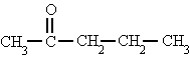
\includegraphics[width=0.4\textwidth]{imagen_19.jpg}
%\centering\captionof{figure}{Pregunta \ref{mon-3}}\label{fig:mon-7}
El alcohol del que proviene del anterior compuesto 
\begin{enumerate}[(A)]
\item 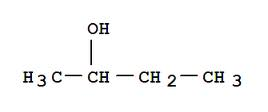
\includegraphics[width=0.4\textwidth]{imagen_20}
\item 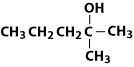
\includegraphics[width=0.35\textwidth]{imagen_21}
\item 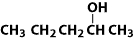
\includegraphics[width=0.35\textwidth]{imagen_22}
\item 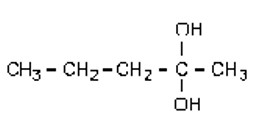
\includegraphics[width=0.4\textwidth]{imagen_23}
\end{enumerate}


%%%%%%%%%%%%%%%%%%%%%%%%%%%%%%%%%%%%%%%%%%
\item La halogenación de alquenos produce la ruptura de su insaturación, por lo que la reacción que mejor representa este proceso es \label{mon-24}


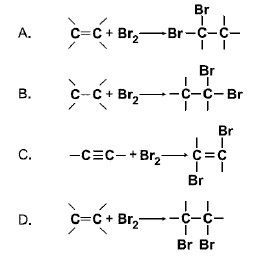
\includegraphics[width=0.4\textwidth]{imagen_24.jpg}
%\centering\captionof{figure}{Pregunta \ref{mon-3}}\label{fig:mon-7}



%%%%%%%%%%%%%%%%%%%%%%%%%%%%%%%%%%%%%%%%%%
\item La fórmula general de los alcanos es C$_n$ + H$_{2n+2}$ siendo n el número de átomos de carbono de la molécula. La fórmula para el butano es  \label{mon-25}\hrulefill\\
\_\hrulefill\\
\_\hrulefill\\
\_\hrulefill.



%%%%%%%%%%%%%%%%%%%%%%%%%%%%%
\end{enumerate}
%%%%%%%%%%%%%%%%%%%%%%%%%%%%%5




\chapterimage{quim2.jpg} % Table of contents heading image

\chapter{Qu\'{i}mica II}\label{chap:quim2}

\begin{enumerate}
%%%%%%%%%
\item  Gracias a los esteres y algunos compuestos aromáticos es posible percibir el olor de las frutas y de las flores, por esto son utilizados para la elaboración de esencias, aromatizantes, perfumes. La esencia de naranja es el acetato de octilo el cual corresponde a la siguiente fórmula: \label{jenn-1}


\begin{enumerate}[(A)]
\item CH$_3$-CH$_2$-COO-(CH$_2$)$_6$-CH$_3$
\item CH$_3$-COO-(CH$_2$)$_7$-CH$_3$
\item CH$_3$-CH$_2$-COO-(CH$_2$)$_5$-CH$_3$
\item CH$_3$-(CH$_2$)$_6$-COO-CH$_2$-CH$_3$
\end{enumerate}


%%%%%%%%%%%%%%%%%%%%%%%%%%%%%


\item La lactosa, azúcar de la leche, es un disacárido, constituido por una molécula de glucosa y una de galactosa. Algunas personas pueden ser intolerantes a este carbohidrato debido a la ausencia de la enzima lactasa, y por ello deben consumir productos deslactosados. Una de las siguientes estructuras corresponde a la lactosa. \label{jenn-2}


\begin{enumerate}[(A)]
\item 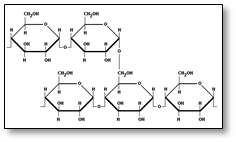
\includegraphics[width=0.35\textwidth]{img1.png}
\item 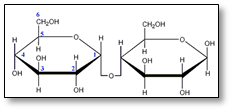
\includegraphics[width=0.35\textwidth]{img2.png}
\item 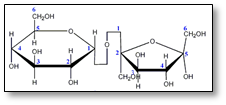
\includegraphics[width=0.35\textwidth]{img3.png}\\
\item \includegraphics[width=0.35\textwidth]{img4.png}
\end{enumerate}


%%%%%%%%%%%%%%%%%%%%%%%%%%%%%


\item  La fuerza que mantiene unidos los átomos entre sí, se le llama enlace químico, el cual le confiere ciertas propiedades a los compuestos formados. De acuerdo con lo anterior son propiedades de los compuestos iónicos:\label{jenn-3}


\begin{enumerate}[(A)]
\item   sólidos a temperatura ambiente y altos puntos de fusión.
\item buenos conductores de la electricidad y poseen brillo metálico.
\item bajos puntos de fusión y de ebullición.
\item malos conductores del calor y la electricidad.
\end{enumerate}


%%%%%%%%%%%%%%%%%%%%%%%%%%%%%


\item  Según el modelo atómico de Bohr, la representación correcta para un elemento que se encuentra ubicado en el grupo IIIA, periodo 3 es:\label{jenn-4}


\begin{enumerate}[(A)]
\item \includegraphics[width=0.25\textwidth]{img5.png}
\item \includegraphics[width=0.25\textwidth]{img6.png}
\item \includegraphics[width=0.25\textwidth]{img7.png}\\
\item \includegraphics[width=0.25\textwidth]{img8.png}
\end{enumerate}


%%%%%%%%%%%%%%%%%%%%%%%%%%%%%


\item   La estructura de Lewis son representaciones de los enlaces químicos, la cual permite explicar la tendencia de los átomos a completar con ocho electrones su última capa. De acuerdo con la anterior información la estructura correcta para el compuesto BCl$_3$ es:\label{jenn-5}


\begin{enumerate}[(A)]
\item \includegraphics[width=0.22\textwidth]{img9.png}
\item \includegraphics[width=0.25\textwidth]{img10.png}
\item \includegraphics[width=0.25\textwidth]{img11.png}\\
\item \includegraphics[width=0.30\textwidth]{img12.png}
\end{enumerate}


%%%%%%%%%%%%%%%%%%%%%%%%%%%%%


\item  6. En la etiqueta de un vino tinto se especifica que este contiene un 13.5 \% de volumen en alcohol, esto quiere decir que el vino contiene:\label{jenn-6}


\begin{enumerate}[(A)]
\item 13.5 g de alcohol por cada 100 mL 
\item  13.5 g de alcohol por cada 100 g
\item  13.5 mL de alcohol por cada 100 mL
\item  13.5 mL de alcohol por cada 100O mL
\end{enumerate}


%%%%%%%%%%%%%%%%%%%%%%%%%%%%%

\subsubsection*{Conteste las preguntas \ref{jenn-7} y \ref{jenn-8} de acuerdo con la siguiente información.}

\item \includegraphics[width=0.45\textwidth]{img13.png}

Respectivamente T = 20$^o$C, H2 = 1 atm, Ar = 3 atm, CO2 = 1 atm.



\item  La temperatura y el volumen que se obtiene al mezclarse los gases en el nuevo cilindro es de:\label{jenn-7}


\begin{enumerate}[(A)]
\item 20$^o$C y 3L
\item  60$^o$C y 3L
\item  60$^o$C y 1L
\item  20$^o$C y 1L
\end{enumerate}


%%%%%%%%%%%%%%%%%%%%%%%%%%%%%


\item Según la teoría de Dalton la presión total de los tres gases al mezclarse es de: \label{jenn-8}


\begin{enumerate}[(A)]
\item    5 atm
\item  1 atm
\item  3 atm
\item  2 atm
\end{enumerate}


%%%%%%%%%%%%%%%%%%%%%%%%%%%%%


\item  El propanoato de calcio es una sal cálcica de fórmula Ca(C2H5COO)2, utilizada como conservante en la elaboración de algunos productos alimenticios como el pan blanco. El grupo funcional al que pertenece es:\label{jenn-9}


\begin{enumerate}[(A)]
\item Acido carboxílico
\item Aldehído
\item Cetona
\item Éster 
\end{enumerate}


%%%%%%%%%%%%%%%%%%%%%%%%%%%%%


\item  La cerveza es una bebida de sabor amargo, producto de la fermentación anaerobia de cereales como la cebada, que por medio de microorganismos como la levadura procesan los carbohidratos como (glucosa, fructosa, sacarosa, almidón entre otros) para obtener alcohol y dióxido de carbono. La reacción que se lleva a cabo en la fermentación alcohólica es la siguiente: C$_6$H$_12$O$_6$ + 2 ADP $\longrightarrow$ 2 CH$_3$-CH$_2$OH + 2 CO$_2$ + 2 ATP + 25.5 kcal \label{jenn-10}\\
De acuerdo con la siguiente información el alcohol que se obtiene es:


\begin{enumerate}[(A)]
\item Etanol
\item Metanol
\item Alcohol propílico
\item Alcohol metílico
\end{enumerate}


%%%%%%%%%%%%%%%%%%%%%%%%%%%%%


\item Según la gráfica de la curva de valoración entre el HCl (un ácido fuerte) y el NaOH (una base fuerte), 
 \label{jenn-11}


\item \includegraphics[width=0.45\textwidth]{img14.png}

El indicador que deja observar claramente el punto de equivalencia en la titulación es:

\begin{enumerate}[(A)]
\item   fenolftaleína
\item rojo de metilo
\item naranja de metilo
\item ninguna de las anteriores
\end{enumerate}


%%%%%%%%%%%%%%%%%%%%%%%%%%%%%


\item  Para la titulación de 25 mL de ácido acético (CH$_3$COOH) se necesitaron 36 mL de hidróxido de potasio (KOH) 0.2 N ¿Cuál es la concentración del ácido acético? \label{jenn-12}


\begin{enumerate}[(A)]
\item   0.3N 
\item 0.5N
\item 1N
\item 0.2N
\end{enumerate}


%%%%%%%%%%%%%%%%%%%%%%%%%%%%%


\item  Para la siguiente reacción  \label{jenn-13}

\begin{equation*}
C_{11}H_{22}O_{11}+O_{2}\longrightarrow CO_{2}+H_{2}O
\end{equation*}

El balanceo correspondiente es,
\begin{enumerate}[(A)]
\item   1;33;11;11
\item 1;11;11;11
\item 1;2;11;22
\item 1;2 ;11;2
\end{enumerate}


%%%%%%%%%%%%%%%%%%%%%%%%%%%%%


\item   La IUPAC es el la Unión Internacional de Química Pura y Aplicada, encargada de establecer las reglas para nombrar los compuestos químicos orgánicos e inorgánicos. De acuerdo a lo anterior el NaClO4, se conoce como:\label{jenn-14}


\begin{enumerate}[(A)]
\item   perclorato de sodio
\item clorato de sodio
\item hipoclorito de sodio
\item clorito de sodio
\end{enumerate}


%%%%%%%%%%%%%%%%%%%%%%%%%%%%%


\item Una reacción de desplazamiento o sustitución es aquella en la que un elemento sustituye y libera a otro elemento presente en el compuesto. De acuerdo con esta información es una reacción de desplazamiento,  \label{jenn-15}


\begin{enumerate}[(A)]
\item $2KClO_{3}\longrightarrow 2KCl + 3O_{2}$
\item $As_{2}O_{3}+4HNO_{3}+H_{2}O$\\ 
 $\longrightarrow\ 2H_{3}AsO_{4}+4NO_{2}$\hfill
\item $Zn + CuSO_{4}+H_{2}O\longrightarrow Cu + ZnSO_{4}$
\item $NaCl+AgNO_{3}\longrightarrow AgCl + NaNO_{3}$
\end{enumerate}


%%%%%%%%%%%%%%%%%%%%%%%%%%%%%


\item  Para las siguientes reacciones, \label{jenn-16}

\begin{align*}
R+O_{2}&\longrightarrow N\\
N+H_{2}O&\longrightarrow U\\
U+HX&\longrightarrow Z+H_{2}O
\end{align*}

De acuerdo con lo anterior $X$ es un no metal, $Z$ es una sal y $U$ es, oxido acido

\begin{enumerate}[(A)]
\item   Oxido básico
\item Ácido oxácido
\item Hidróxido
\end{enumerate}


%%%%%%%%%%%%%%%%%%%%%%%%%%%%%


\item En el compuesto Cl$_2$O$_3$, los estados de oxidación del cloro y del oxígeno son respectivamente, \label{jenn-17}


\begin{enumerate}[(A)]
\item   -2, +2   
\item +2, -2                         
\item -3, +2    
\item   +3, -2
\end{enumerate}


%%%%%%%%%%%%%%%%%%%%%%%%%%%%%


\item  La tabla muestra el porcentaje en peso de unos iones presentes en dos muestras de agua tomados de dos lugares diferentes,\label{jenn-18}

\begin{center}
\begin{tabular}{c|cc}
\hline 
\hline 
 & \multicolumn{2}{c}{Porcentaje en peso}   \\ 
Iones & Muestra 1 & Muestra 2 \\ 
\hline 
\hline 
K$^{+}$ & 4.25 & 0 \\		 
Na$^{++}$ & 6.36 & 0 \\ 
Ca$^{++}$ & 7.38 & 0 \\ 
Cl$^{-}$ & 16.25 & 12.00 \\ 
\hline 
\end{tabular} 
\end{center}

\begin{enumerate}[(A)]
\item   CaNa$_2$; CaK$_2$; CaCl$_2$
\item NaK; CaCl$_2$; NaKCl
\item NaCl; KCl; CaCl$_2$
\item NaCa; KCa; KCl$_2$
\end{enumerate}


%%%%%%%%%%%%%%%%%%%%%%%%%%%%%


\item  La isomería es una propiedad de los compuestos químicos, en el cual se presenta una misma fórmula molecular pero con estructura u organización diferente de los átomos. De este modo es un isómero del ácido 2-hidroxihexanoico \label{jenn-19}


\begin{enumerate}[(A)]
\item \includegraphics[width=0.35\textwidth]{img15.png}
\item \includegraphics[width=0.32\textwidth]{img16.png}
\item \includegraphics[width=0.38\textwidth]{img17.png}\\
\item \includegraphics[width=0.3\textwidth]{img18.png}
\end{enumerate}


%%%%%%%%%%%%%%%%%%%%%%%%%%%%%


\item La aspirina o acido acetilsalicilico, es uno de los principales analgesicos a nivel mundial, \label{jenn-20}

\begin{center}
\includegraphics[width=0.30\textwidth]{img19.jpeg}
\end{center}

Químicamente, las funciones que integran la estructura de la aspirina es,


\begin{enumerate}[(A)]
\item   Benceno, éster y acido carboxílico
\item Fenol, cetona y acido carboxílico
\item Aldehído, éter y benceno
\item Aldehído, cetona y benceno
\end{enumerate}


%%%%%%%%%%%%%%%%%%%%%%%%%%%%%


\item El reactivo de Lugol es una disolución entre yodo molecular (I2) y yoduro potásico (KI), el cual es utilizado para la identificación de polisacáridos como el almidón. ¿Por qué el reactivo de Lugol presenta una coloración azul oscura o negra en presencia de almidón? \label{jenn-21}\hrulefill\\
\_\hrulefill\\
\_\hrulefill\\
\_\hrulefill.



%%%%%%%%%%%%%%%%%%%%%%%%%%%%%


\item   ¿Qué diferencia hay entre una solución homogénea y un coloide?\label{jenn-22}\hrulefill\\
\_\hrulefill\\
\_\hrulefill\\
\_\hrulefill.


%%%%%%%%%%%%%%%%%%%%%%%%%%%%%


\item ¿Qué es un polímero? \label{jenn-23}\hrulefill\\
\_\hrulefill\\
\_\hrulefill\\
\_\hrulefill.



%%%%%%%%%%%%%%%%%%%%%%%%%%%%%


\item  Los aldehídos presentan reacciones de oxidación, de acuerdo con la anterior información si se oxida el 2-metil-hexanal¿ Cuál es el compuesto que se forma \label{jenn-24}\hrulefill\\
\_\hrulefill\\
\_\hrulefill\\
\_\hrulefill.





%%%%%%%%%%%%%%%%%%%%%%%%%%%%%


\item  En la determinación de la cantidad de sustancia que se produce durante una reacción química, es necesario conocer el reactivo limite, ¿Por qué es necesario conocerlo?
\label{jenn-25}\hrulefill\\
\_\hrulefill\\
\_\hrulefill\\
\_\hrulefill.








%%%%%%%%%%%%%%%%%%%%%%%%%%%%%
\end{enumerate}
%%%%%%%%%%%%%%%%%%%%%%%%%%%%%5


%%%%%%%%%%%%%%%%%%%%%%%%%%%%%%%%%%%%%%%%%%%%%%%%%%
%%%%%%%%%%%%     Ciencias Biolog´ia %%%%%%%%%%%%%%
%%%%%%%%%%%%%%%%%%%%%%%%%%%%%%%%%%%%%%%%%%%%%%%%%%
\chapterimage{bio1.jpg} % Table of contents heading image

\chapter{Biolog\'{i}a}\label{chap:bio1}
\begin{enumerate}



\item Las plantas que poseen flores se originan por reproducción  sexual. En este proceso siempre intervienen dos componentes: uno masculino y otro femenino. Siguiendo el esquema   de la derecha que representa la fecundación vegetal en los momentos I y II, usted diría que este proceso ocurre exactamente cuándo: \label{bio-2}
\begin{center}
\includegraphics[width=0.45\textwidth]{bio_1.jpg} 
\end{center}
\begin{enumerate}[(A)]
\item El grano de polen se deposita sobre el estigma.
\item El polen se une con el óvulo en el ovario.
\item El óvulo madura y es el único componente que interviene.
\item El polen se une con el óvulo en el tubo polínico.
\end{enumerate}


%%%%%%%%%%%%%%%%%%%%%%%%%%%%
\newpage
\item La reproducción asexual se presenta    principalmente en tres modalidades. Cuando en la pared del progenitor se forma un brote o yema se desarrolla y se transforma en un nuevo individuo que se separa para vivir independientemente se conoce con el nombre de: \label{bio-1}
\begin{enumerate}[(A)]
\item Reproducción sexual 
\item Fecundación externa 
\item Gemación 
\item Regeneración 
\end{enumerate}
%%%%%%%%%%%%%%%%%%%%%%%%%%%%%%%%%%%%%%%%%%%%
\item En una especie de planta, el gen para flores rojas ($R$) es dominante sobre el gen para flores blancas ($r$). El siguiente cuadro de Punnett muestra el cruce entre una planta pura (homocigota) con flores rojas y una planta pura con flores blancas: \label{bio-3}\\[-1.1cm]
\begin{center}
\includegraphics[width=0.45\textwidth]{bio_2.jpg} 
\end{center}
En el cuadro de Punnet las letras $R$ y $r$ simbolizan los alelos del gen para el color. Un alelo queda en cada gameto debido al proceso de 
\begin{enumerate}[(A)]
\item Meiosis.
\item Mitosis.
\item Fecundación.
\item Reproducción asexual.
\end{enumerate}
%%%%%%%%%%%%%%%%%%%%%%%%%%%%%%%%%%%%%
\item En los guisantes el gen que determina el color amarillo (A) domina sobre el que determina el color verde (a) que es recesivo. En el esquema  se representa: \label{bio-4}

\begin{center}
\includegraphics[width=0.35\textwidth]{bio_3.jpg} 
\end{center}
\begin{enumerate}[(A)]
\item La primera ley de Mendel.
\item La segunda ley de Mendel.
\item La tercera ley de Mendel.
\item Un cruce dihíbrido.
\end{enumerate}

%%%%%%%%%%%%%%%%%%%%%%%%%%%%%%%%%%%%%%%%%%%
\item Observa los siguientes dibujos: \label{bio-5}

\begin{center}
\includegraphics[width=0.5\textwidth]{bio_4} 
\end{center}

Según estas dos cadenas, ¿Cuales seres vivos ocupan el mismo nivel trófico?

\begin{enumerate}[(A)]
\item  as hormigas y el pasto.
\item El venado y el gato.
\item El cocodrilo y el gato.
\item El cocodrilo y el ratón.
\end{enumerate}


%%%%%%%%%%%%%%%%%%%%%%%%%%%%%%%%%%%%%%%%%%%%%%%%
\newpage
\item En una isla (A) se encuentra una especie de lagartijas conformadas por hembras. Por esta razón la reproducción es asexual y en consecuencia las hijas son una copia idéntica de la madre.  Por otro lado, en una isla cercana (B) hay otra especie de lagartijas con machos y hembras que se reproducen sexualmente.  La siguiente grafica representa la población de lagartijas en cada una de las islas:\label{bio-6}

Si una enfermedad comienza a provocar la muerte de las poblaciones de lagartijas en las islas ¿en cuál de ellas es más  probable que la población de lagartijas sobreviva?.


\begin{center}
\includegraphics[width=0.45\textwidth]{bio_5.jpg} 
\end{center}
\begin{enumerate}[(A)]
\item En la isla A porque todas las lagartijas son genéticamente iguales.
\item En la isla A porque las hembras son más resistentes.
\item En la isla B porque la variabilidad genética de las lagartijas es alta. 
\item En la isla b porque las lagartijas macho son m\'as fuertes.
\end{enumerate}

%%%%%%%%%%%%%%%%%%%%%%%%%%%%%%%%%%%%%%%%%%%%%%%%%%%%%%%%%%%%5
\newpage
\subsubsection*{Responda las preguntas \ref{bio-7} y \ref{bio-8} de acuerdo con la siguiente información}
Una especie de mono presentaba alta tasa de predación debido a su poca agilidad para escapar de sus depredadores. En un momento de su historia evolutiva surgieron individuos con brazos más largos que lograron huir con más facilidad. En la actualidad la mayoría de los monos de dicha especie presentan brazos largos.


%%%%%%%%%%%%%%%%%%%%%%%%%%%%%%%%%%%%%%%%%%%%%5
\item  Según los principios de Darwin y analizando la evolución de dicha especie de monos se podría plantear que con mayor probabilidad: \label{bio-7}

\begin{enumerate}[(A)]
\item En una época determinada la característica de los brazos largos apareció simultáneamente en la mayoría de los individuos, los cuales al reproducirse heredaron esta característica a sus hijos.
\item El tamaño largo de los brazos se logró poco a poco y de manera individual a medida que los monos huían de sus depredadores, los actuales monos de brazos largos son producto de la ejercitación de los brazos.
\item El tamaño largo de los brazos fue una característica que apareció al azar, se heredó y afectó el éxito reproductivo de generación en generación hasta que la mayor parte de los individuos de esta especie tuvieron brazos largos.
\item Los brazos largos los obtuvieron algunos individuos al azar, característica que no se heredó por carecer de utilidad para la especie.
\end{enumerate}

%%%%%%%%%%%%%%%%%%%%%%%%%%%%%%%%%%%%%%%%%%%%%%%%%%%%%%%%%%%%%%%%%%%
\newpage
\item En la actualidad, esta especie de mono es exitosa en bosques húmedos tropicales. Debido a sus movimientos estos monos deben consumir diariamente gran cantidad de energía, por lo que requieren una dieta rica en calorías. De las siguientes, la dieta que mejor se acomodaría a los requerimientos de estos monos sería: \label{bio-8}

\begin{center}
\includegraphics[width=0.45\textwidth]{bio_6.jpg} 
\end{center}


%%%%%%%%%%%%%%%%%%%%%%%%%%%%%%%%%%%%%%%%%%%%%%%%%%%%%%%%%%%%%%%%%%%
\item El siguiente dibujo muestra un experimento en el que se sembraron plantas en soluciones que contenían diferentes nutrientes. \label{bio-9}

\begin{center}
\includegraphics[width=0.45\textwidth]{bio_7.jpg} 
\end{center}

La pregunta que puede responderse con base en los resultados de este experimento es:

\begin{enumerate}[(A)]
\item ¿Cuál  es el efecto de cada nutriente en la absorción de agua en las plantas?
\item ¿Cuál  es el efecto de cada nutriente en el desarrollo de las plantas?
\item ¿Cuál  es el nivel mínimo de nutrientes en que una planta puede crecer?
\item ¿Cuál  eses el efecto del agua en la absorción de nutrientes en las plantas?
\end{enumerate}

%%%%%%%%%%%%%%%%%%%%%%%%%%%%%%%%%%%%%%%%%%%%%%%%%%%%%%%%%%%%%%%%%%%
\newpage
\item Los receptores sensosiales son parte del sistema nerviosdos de los animales y les permiten a estos percibir el ambiente.  Se metio un raton en un  cuarto oscuro donde habia un trozo de queso con olor agradable para el animal.  ¿Cuáles fueron los receptores sensoriales que uso el ratón para llegar al queso? \label{bio-10}

\begin{enumerate}[(A)]
\item Quimiorreceptores y termorreceptores.
\item Mecanorreceptores y receptores de dolor.
\item Termorreceptores y fotorreceptores.
\item Quimiorreceptores y mecanorreceptores.
\end{enumerate}


\subsubsection*{Las preguntas \ref{bio-11} a la \ref{bio-13}  se contestan teniendo en cuenta la siguiente lectura}

Las enfermedades de transmisión sexual (ETS), causadas por virus, bacterias, protistas o artrópodos que infectan los órganos sexuales o el aparato reproductor representan un serio y creciente problema de salud en todo el mundo. La Organización Mundial de la Salud calcula que hay 250 millones de casos nuevos de ETS cada año. Como su nombre lo dice, estas enfermedades se transmiten ya sea exclusiva o principalmente a través del contacto sexual. 


Algunas de las enfermedades más comunes de este tipo son: 
Infecciones bacterianas, la gonorrea, una infección del aparato genital y urinario, es una de las más comunes de todas las enfermedades infecciosas y se calcula que infecta a por lo menos dos millones de personas cada año. 

La bacteria causante, la cual no puede sobrevivir fuera del cuerpo, se transmite casi exclusivamente por contacto íntimo. Penetra las membranas limitantes de la uretra, ano, cérvix, útero, oviductos y garganta. En los hombres, la inflamación de la uretra da como resultado la salida de pus por el pene y una micción dolorosa, Aproximadamente el 10\% de los hombres infectados y 50\% de las mujeres infectadas tienen síntomas ligeros o ausentes y, por tanto, no buscan tratamiento. Se convierten en portadores quienes pueden diseminar fácilmente la enfermedad. La gonorrea puede ocasionar infertilidad al bloquear los oviductos con tejido cicatrizante. El tratamiento con penicilina en un principio fue muy satisfactorio, pero las cepas resistentes ahora requieren el uso de otros antibióticos. Los niños nacidos de madres infectadas pueden adquirir la bacteria durante el parto. La bacteria ataca a los ojos de los recién nacidos y en alguna ocasión representó una causa importante de ceguera. Hoy en día, a la mayoría de los nacidos se les administran inmediatamente gotas con antibiótico para matar esta bacteria. 

%%%%%%%%%%%%%%%%%%%%%%%%%%%%%%%%%%%%%%%%%%%%%%%%%%%%%%%%%%%%%%%%%%%
\item La gonorrea, una infección del aparato genital y urinario, es una de las más comunes de todas las enfermedades infecciosas, en su etapa inicial: \label{bio-11}

\begin{enumerate}[(A)]
\item Afecta los ojos de los recién nacidos y en alguna ocasión representó una causa importante de ceguera. 
\item Penetra las membranas limitantes de la uretra, ano, cérvix, útero, oviductos y garganta.
\item Puede ocasionar infertilidad al bloquear los oviductos con tejido cicatrizar. 
\item Los niños nacidos de madres infectadas pueden adquirir la bacteria durante el parto. 
\end{enumerate}


%%%%%%%%%%%%%%%%%%%%%%%%%%%%%%%%%%%%%%%%%%%%%%%%%%%%%%%%%%%%%%%%%%%
\item Para combatir la gonorrea se utiliza: \label{bio-12}

\begin{enumerate}[(A)]
\item Penicilina y analgésicos. 
\item Penicilina y barbitúricos. 
\item Penicilina y antibióticos. 
\item Penicilina y calmantes. 
\end{enumerate}

%%%%%%%%%%%%%%%%%%%%%%%%%%%%%%%%%%%%%%%%%%%%%%%%%%%%%%%%%%%%%%%%%%%
\item  Las enfermedades de transmisión\\ sexual (ETS), son causadas por:\label{bio-13}

\begin{enumerate}[(A)]
\item Vírus, leveduras, protistas o\\ garrapatas. 
\item Vírus, bactérias, protistas o\\ artrópodos. 
\item Vírus, bactérias, nematódeos o\\ artrópodos. 
\item Vírus, hongos, protistas o\\ garrapatas.
\end{enumerate}

%%%%%%%%%%%%%%%%%%%%%%%%%%%%%%%%%%%%%%%%%%%%%%%%%%%%%%%%%%%%%%%%%%%
\item En la figura se muestra  la localización  del gen que produce una proteína en humanos. Cuándo este gen muta (figura    derecha), produce una proteína diferente de la proteína normal. Lo que determina la proteína que produce el gen es:  \label{bio-14}
\begin{center}
\includegraphics[width=0.45\textwidth]{bio_8.jpg} 
\end{center}
\begin{enumerate}[(A)]
\item El  cromosoma  al  que pertenece  el gen.
\item La secuencia de  nucleótidos  que posee.
\item Su  localización dentro   del cromosoma.
\item La  configuración  helicoidea el ADN.	
\end{enumerate}


%%%%%%%%%%%%%%%%%%%%%%%%%%%%%%%%%%%%%%%%%%%%%%%%%%%%%%%%%%%%%%%%%%%
\newpage
\item Unos   investigadores  evaluaron  la relación ecológica de los insectos consumidores de néctar y una planta de interés comercial.  Como resultado  reportaron los datos  en las siguientes gráficas \label{bio-15}
\begin{center}
\includegraphics[width=0.45\textwidth]{bio_9.jpg} 
\end{center}
A partir   de las  gráficas.  Una de las  relaciones  que  se puede  proponer  entre los insectos y planta  es   que los insectos:
\begin{enumerate}[(A)]
\item Dispersan los frutos de la planta.
\item Se alimenta de las hojas de la planta.
\item Polinizan la  planta.
\item Nutren la   planta.
\end{enumerate}


%%%%%%%%%%%%%%%%%%%%%%%%%%%%%%%%%%%%%%%%%%%%%%%%%%%%%%%%%%%%%%%%%%%
\newpage
\item Los  antibióticos   son sustancias  químicas  que impiden  el  crecimiento de   las  bacterias.  Por  sus  características, los  antibióticos  se   utilizan   para tratar   infecciones.  Sin  embargo, algunos  microrganismos  pueden   ser  resistentes  y trasmitirlo   a  su descendencia.  Una  forma  de evitar  la  resistencia a los antibióticos   por parte   de los  microorganismos   es: \label{bio-16}


\begin{enumerate}[(A)]
\item Utilizar  otros  medicamentos  regulares.
\item Seguir  el tratamiento  recomendado para  el antibiótico.
\item No utilizar  antibiótico.
\item Evitar  el contacto  con las bacterias resistentes.
\end{enumerate}


%%%%%%%%%%%%%%%%%%%%%%%%%%%%%%%%%%%%%%%%%%%%%%%%%%%%%%%%%%%%%%%%%%%
\item  Observe el siguiente  modelo  del flujo   de la energía  en un ecosistema. \label{bio-18}
\begin{center}
\includegraphics[width=0.45\textwidth]{bio_11.jpg} 
\end{center}
Según  el modelo se puede  concluir   que  este ecosistema es  un sistema  abierto ¿por qué?
\begin{enumerate}[(A)]
\item Los seres vivos usan el alimento para transformarlo en energía.
\item Varios  nutrientes  pueden salir por  lixiviados  a otros ecosistemas.
\item Los descomponedores  trasforman  los desechos   en nutrientes  para las plantas.
\item La energía fluye  a través  de los niveles    tróficos.
\end{enumerate}
%%%%%%%%%%%%%%%%%%%%%%%%%%%%%%%%%%%%%%%%%%%%%%%%%%%%%%%%%%%%%%%%%%%
\item Las  abejas  tienen un  completo   sistema   de   dos  pares  de  alas   unidas    entre  sí    que  se mueven  al tiempo,   como se  observa  en el siguiente  dibujo. \label{bio-17}
\begin{center}
\includegraphics[width=0.45\textwidth]{bio_10.jpg} 
\end{center}
Para  lograr  el vuelo rápido las  abejas  necesitan:
\begin{enumerate}[(A)]
\item Músculos  para mover  las  alas.
\item Exoesqueleto  articulado  que permita flexibilidad de durante  el  vuelo.
\item Hormonas para estimular el movimiento.
\item  Venas en las alas que  le den rigidez.
\end{enumerate}



%%%%%%%%%%%%%%%%%%%%%%%%%%%%%%%%%%%%%%%%%%%%%%%%%%%%%%%%%%%%%%%%%%%
\newpage
\item El dióxido de carbono (CO2) se reconoce  como el gas  más  importante junto al  metano  y los   hidroflurocarbonos  en el calentamiento global. La actividad  humana  ha llevado  al    incremento de  este gas en la atmósfera, aunque las plantas y las algas fijan este gas  disminuyendo su  concentración.  Se determinó  el aporte del CO2  a la atmósfera en 4  zonas y los resultados se mostraron  en la siguiente gráfica. \label{bio-19}


\begin{center}
\includegraphics[width=0.45\textwidth]{bio_12.jpg} 
\end{center}
Según los resultados anteriores,  a  que corresponde   cada  una de las zonas en la gráfica: 

\begin{enumerate}[(A)]
\item Zona 1: Océano.   Zona 2: Bosque. Zona 3: Rular.    Zona 4: Fabricas.
\item Zona 1: Bosque.   Zona 2: Rural.  Zona 3: Fabricas. Zona 4: Océano.
\item Zona 1: Fabricas. Zona 2: Rural.  Zona 3: Bosque.   Zona 4: Oceano.
\item Zona 1: Bosque.   Zona 2: Océano. Zona 3: Rural.    Zona 4: Fabric.
\end{enumerate}


%%%%%%%%%%%%%%%%%%%%%%%%%%%%%%%%%%%%%%%%%%%%%%%%%%%%%%%%%%%%%%%%%%%
\newpage
\item Entre  los  años  de  1845 y 1852, todos  los  cultivos  de papa  de  la isla de  Irlanda  fueron   destruidos por  una enfermedad  producida por un  hongo. Dos factores  contribuyen  a la  alta  dispersión de  la  enfermedad: \label{bio-20}
(1)en Irlanda  se cultivaba únicamente una variedad de papa y (2) los  cultivos  de papa  se  encontraban aislados del resto de  mundo, por lo  cual se producía únicamente entre sí.
Desde un punto de  vista genético estos  2  factores contribuyeron  a la dispersión de la enfermedad por qué:
\begin{enumerate}[(A)]
\item Se  redujo  la variedad  genética de los cultivos  de papa  haciéndolos susceptibles a la epidemia.
\item Produjeron una alta  variedad  genética  generando plantas  de  papas  muy  diferentes entre  si  y  susceptibles  a la epidemia.
\item El genoma     del  hongo  se incorporó rápidamente  al  ADN  de las papas y la enfermedad  se trasmitió genéticamente.
\item Ocasiones  un   aumento  en  el número  de  cromosomas  de  las  papas  cultivadas, haciéndolas    susceptibles  a   la  epidemia.
\end{enumerate}

%%%%%%%%%%%%%%%%%%%%%%%%%%%%%%%%%%%%%%%%%%%%%%%%%%%%%%%%%%%%%%%%%%%
\item Observa la  figura \label{bio-22}\\[-1.1cm]
\begin{center}
\includegraphics[width=0.45\textwidth]{bio_13.jpg} 
\end{center}
Las  flechas    en la figura    muestran  la membrana   interdactilar  que se encuentra en las extremidades de animales  como ranas  acuáticas patos    y ornitorrincos. Está membrana  es común   en estos  animales ¿por qué?
\begin{enumerate}[(A)]
\item Descienden   de  un ancestro común  cercano.
\item Evolucionaron al mismo tiempo.
\item Se desplazan en medios acuáticos.
\item Les sirve para agarrar la presa.
\end{enumerate}
%%%%%%%%%%%%%%%%%%%%%%%%%%%%%%%%%%%%%%%%%%%%%%%%%%%%%%%%%%%%%%%%%%%
\item El  alcohol   es  una  sustancia  que  puede generar  dependencia en  las  personas  que  lo  consumen, inhibe  la  producción  de glóbulos blancos, genera un deterioro  de las mucosas  del   sistema  digestivo , incrementa la  actividad  cardiaca  y  altera la acción  de  algunos  neurotransmisores. \label{bio-21}

De  acuerdo  con  lo  anterior,  cuál  de las  siguientes  alteraciones en  la  salud , estaría  relacionada  con el consumo  excesivo  de  alcohol.

\begin{enumerate}[(A)]
\item Ser  propenso a contraer  infecciones  bacterianas o  virales.
\item Tener  una baja producción  de  gástricos  en el estómago.
\item Aumentar  el  estado  de  alerta  y la  velocidad  de los  reflejos.
\item Reducir significativamente  la  presión   arterial.
\end{enumerate}

%%%%%%%%%%%%%%%%%%%%%%%%%%%%%%%%%%%%%%%%%%%%%%%%%%%%%%%%%%%%%%%%%%%
\item Observe la siguiente red alimenticia que existe en un ecosistema. Teniendo en cuenta las relaciones establecidas en la anterior red alimentaria, ¿Qué se espera que suceda con la población de sapos si todos los peces pequeños se extinguen? ¿Por qué? \label{bio-25}
\begin{center}
\includegraphics[width=0.45\textwidth]{bio_14.jpg} 
\end{center}
Para responder esta pregunta lo debe hacer en las líneas siguientes sin salirse del recuadro, debe ser clara y concisa  \hrulefill\\
\_\hrulefill\\
\_\hrulefill\\
\_\hrulefill\hrulefill\\
\_\hrulefill

%%%%%%%%%%%%%%%%%%%%%%%%%%%%%%%%%%%55
\newpage
\item La  leshmaneasis  es una  enfermedad   tropical   cuyos   síntomas     característicos   son ulceras cutáneas   e inflamación del  hígado  y del bazo.  Se  trasmite  principalmente   por la picadura   de  insectos  hematófagos    que  inyectan en la victima  un   protozoario  del  genero Leishmania, aunque también  puede trasmitirse por transfusiones   de  sangre infectadas    o con  congénitamente.  A partir  de esta información sobre la leishmaniasis  ¿Cuál de las  siguientes preguntas  puede resolverse      en una investigación de ciencias naturales?  \label{bio-23}       


\begin{enumerate}[(A)]
\item ¿Qué   ideas   y  concepciones  sobre el  ciclo de  vida de los  insectos hematófagos tiene las culturas   de los   países   afectados   por leishmaneasis?
\item ¿Cómo fluye  la presencia  de leishmaniasis   en el ingreso  per cápita  de los  países  de la región   ecuatorial?
\item ¿Por qué se inflama el hígado  y el bazo   de las personas  que han  sido infectadas con Leishmania?
\item ¿Qué políticas  deben    adoptarse    para l  asignación   de  recursos   para el control  de la enfermedad?
\end{enumerate}


%%%%%%%%%%%%%%%%%%%%%%%%%%%%%%%%%%%%%%%%%%%%%%%%%%%%%%%%%%%%%%%%%%%
\newpage
\item Durante la fotosíntesis, los estomas en las hojas permanecen abiertos  el tiempo suficiente para captar dióxido de carbono, lo que a su vez genera  una pérdida de agua por transpiración.  Los espacios que deja el agua transpirada tienen que ocuparse nuevamente  por moléculas de agua nueva, que ascienden a las hojas desde las raíces a través del xilema. Según esta información, se puede afirmar que los estomas son importantes en el proceso de nutrición de las plantas, porque: \label{bio-24}

\begin{enumerate}[(A)]
\item Son células especializadas en la absorción de sales minerales.
\item Por ellos ingresan sales que se distribuyen a toda la planta a través del xilema.
\item Cuando están abiertos permiten que el agua suba con iones para las células.
\item Permiten el flujo de sabia elaborada por el xilema.  
\end{enumerate}


%%%%%%%%%%%%%%%%%%%%%%%%%%%%%%%%%%%%%%%%%%%%%%%%%%%%%%%%%%%%%%%%%%%



%%%%%%%%%%%%%%%%%%%%%%%%%%%%%
\subsubsection*{Responda las preguntas \ref{bio-26} y \ref{bio-27} a partir de la  siguiente lectura}


\noindent Las bacterias son células procariotas sin núcleo definido en su interior. Su tamaño es unas diez veces inferior  de las células eucariotas. En su estructura podemos observar los siguientes componentes:\\
La pared bacteriana es una envoltura rígida y permeable, que da forma a las células bacterianas está rodeada por la membrana plasmática. Existen dos tipos de pared: Gram positiva y Gram negativa. La pared Gram positiva es monoestraficada, está formada por una capa basal de peptidoglucanos (mureína), a la cual se asocian polisacáridos, ácidos teicoicos y proteínas. La pared Gram negativa es biestratificada, con una capa basal de peptidoglucanos rodeada de una bicapa lipídica que además contiene fosfolípidos, polisacáridos y proteínas.\\

La membrana plasmática es una bicapa lipídica con proteínas, similar a la de las células eucariotas, pero más fluida. Mesosomas: la membrana presenta invaginaciones hacia el interior, en esta zona se encuentran las enzimas responsables de la respiración celular.  En el plasma del interior de las bacterias se encuentran los ribosomas que son más pequeños que los de las células eucariotas. Su función es la síntesis de proteínas. El cromosoma bacteriano es una molécula de ADN circular de doble cadena asociado con unas pocas proteínas que está anclado en un punto de la membrana plasmática.  Algunas bacterias tienen flagelos que sirven para el movimiento, otras tienen fimbrias o pelos  que sirven para adherirse a superficies.\\

Formas de nutrición en función de la fuente de carbono que utilicen las bacterias se dividen en:\\

\textbf{Autótrofas:} utilizan el CO2 como fuente de carbono para construir a partir de él todas sus biomoléculas orgánicas.\\

\textbf{Heterótrofas:} utilizan el carbono de moléculas orgánicas ya elaboradas por otros seres vivos.\\

Según la fuente de energía que utilizan, las bacterias pueden ser:\\

\textbf{Fotótrofas o fotosintéticas:} utilizan como fuente de energía la luz solar.\\

\textbf{Quimiótrofas o quimiosintéticas:} utilizan la energía liberada en las reacciones químicas exotérmicas, reacciones de óxido-reducción.


%%%%%%%%%%%%%%%%%%%%5
\newpage
\item Son componentes importantes de la estructura de una bacteria:\label{bio-26}


\begin{enumerate}[(A)]
\item Cílios, pelos, núcleo, ribosomas.
\item Pared, La membrana plasmática, el plasma, ADN.
\item Gram positiva y Gram negativa, ácidos teicoicos y proteínas.
\item Bicapa lipídica, fosfolípidos, polisacáridos y proteínas.
\end{enumerate}


%%%%%%%%%%%%%%%%%%%%%%%%%%%%%
\newpage
\item En relación a la forma de nutrición de las bacterias es correcto afirmar: \label{bio-27}


\begin{enumerate}[(A)]
\item Las bacterias autótrofas y heterótrofas utilizan el alimento presente en la atmósfera.
\item  Las bacterias Fotótrofas o fotosintéticas,  utilizan como fuente de energía el agua.
\item  Quimiótrofas o quimiosintéticas: utilizan la energía liberada en las reacciones químicas      exotérmicas, reacciones de óxido-reducción.
\item  Las bacterias son descomponedoras.
\end{enumerate}

%%%%%%%%%%%%%%%%%%%%%%%%%%%%%
\end{enumerate}
%%%%%%%%%%%%%%%%%%%%%%%%%%%%%

\let\cleardoublepage\clearpage
\newpage
%%%%%%%%%%%%%%%%%%%%%%%%%%%%%%%%%%%%%%%%%%%%%%%%%%
%%%%%%%%%%%% Hoja de Respuesta%%%%%%%%%%%%%%%%%%%%
%%%%%%%%%%%%%%%%%%%%%%%%%%%%%%%%%%%%%%%%%%%%%%%%%%
\let\cleardoublepage\clearpage

\onecolumn
\setlength{\headsep}{-80pt}
\chapterimage{blanck.jpg}
\chapter{Hoja de Respuestas}

\newcommand*\mycirc[1]{%
  \begin{tikzpicture}
    \node[draw,circle,inner sep=1pt,minimum width=.5cm]  (bigc) {#1};
  \end{tikzpicture}}
%\mycirc{N}
%\mycirc{F}



%\section*{
%{\fontsize{40}{60}\selectfont Hoja de Respuestas}}
\renewcommand{\arraystretch}{2.}

\begin{center}
\begin{tabular}[t]{|c|c|c|c|c|c|c|c|}
\cline{1-2}\cline{4-5}\cline{7-8}
Pregunta &  Respuesta & &Pregunta &  Respuesta && Pregunta &  Respuesta \\
\cline{1-2}\cline{4-5}\cline{7-8}
1. & \mycirc{a} \mycirc{b} \mycirc{c} \mycirc{d} && 21. & \mycirc{a} \mycirc{b} \mycirc{c} \mycirc{d}  && 41 & \mycirc{a} \mycirc{b} \mycirc{c} \mycirc{d}  \\
2. & \mycirc{a} \mycirc{b} \mycirc{c} \mycirc{d} && 22. & \mycirc{a} \mycirc{b} \mycirc{c} \mycirc{d}  && 42. & \mycirc{a} \mycirc{b} \mycirc{c} \mycirc{d}  \\
3.  & \mycirc{a} \mycirc{b} \mycirc{c} \mycirc{d} && 23. & \mycirc{a} \mycirc{b} \mycirc{c} \mycirc{d}  && 43. & \mycirc{a} \mycirc{b} \mycirc{c} \mycirc{d}  \\
4.   & \mycirc{a} \mycirc{b} \mycirc{c} \mycirc{d} && 24. & \mycirc{a} \mycirc{b} \mycirc{c} \mycirc{d}  && 44. & \mycirc{a} \mycirc{b} \mycirc{c} \mycirc{d}  \\
 5.   & \mycirc{a} \mycirc{b} \mycirc{c} \mycirc{d} && 25. & \mycirc{a} \mycirc{b} \mycirc{c} \mycirc{d}  && 45. & \mycirc{a} \mycirc{b} \mycirc{c} \mycirc{d}  \\
6.     & \mycirc{a} \mycirc{b} \mycirc{c} \mycirc{d} && 26. & \mycirc{a} \mycirc{b} \mycirc{c} \mycirc{d}  && 46. & \mycirc{a} \mycirc{b} \mycirc{c} \mycirc{d}  \\
7.      & \mycirc{a} \mycirc{b} \mycirc{c} \mycirc{d} && 27. & \mycirc{a} \mycirc{b} \mycirc{c} \mycirc{d}  && 47. & \mycirc{a} \mycirc{b} \mycirc{c} \mycirc{d}  \\
  8.     & \mycirc{a} \mycirc{b} \mycirc{c} \mycirc{d} && 28. & \mycirc{a} \mycirc{b} \mycirc{c} \mycirc{d}  && 48. & \mycirc{a} \mycirc{b} \mycirc{c} \mycirc{d}  \\
9.    & \mycirc{a} \mycirc{b} \mycirc{c} \mycirc{d} && 29. & \mycirc{a} \mycirc{b} \mycirc{c} \mycirc{d}  && 49. & \mycirc{a} \mycirc{b} \mycirc{c} \mycirc{d}  \\
10.   & \mycirc{a} \mycirc{b} \mycirc{c} \mycirc{d} && 30. & \mycirc{a} \mycirc{b} \mycirc{c} \mycirc{d}  && 50. & \mycirc{a} \mycirc{b} \mycirc{c} \mycirc{d}  \\
11.  & \mycirc{a} \mycirc{b} \mycirc{c} \mycirc{d} && 31. & \mycirc{a} \mycirc{b} \mycirc{c} \mycirc{d}  && 51. & \mycirc{a} \mycirc{b} \mycirc{c} \mycirc{d}  \\
12.   & \mycirc{a} \mycirc{b} \mycirc{c} \mycirc{d} && 32. & \mycirc{a} \mycirc{b} \mycirc{c} \mycirc{d}  && 52. & \mycirc{a} \mycirc{b} \mycirc{c} \mycirc{d}  \\
13.  & \mycirc{a} \mycirc{b} \mycirc{c} \mycirc{d} && 33. & \mycirc{a} \mycirc{b} \mycirc{c} \mycirc{d}  && 53. & \mycirc{a} \mycirc{b} \mycirc{c} \mycirc{d}  \\
 14. & \mycirc{a} \mycirc{b} \mycirc{c} \mycirc{d} && 34. & \mycirc{a} \mycirc{b} \mycirc{c} \mycirc{d}  && 54. & \mycirc{a} \mycirc{b} \mycirc{c} \mycirc{d}  \\
15. & \mycirc{a} \mycirc{b} \mycirc{c} \mycirc{d} && 35. & \mycirc{a} \mycirc{b} \mycirc{c} \mycirc{d}  && 55. & \mycirc{a} \mycirc{b} \mycirc{c} \mycirc{d}  \\
16.  & \mycirc{a} \mycirc{b} \mycirc{c} \mycirc{d} && 36. & \mycirc{a} \mycirc{b} \mycirc{c} \mycirc{d}  && 56. & \mycirc{a} \mycirc{b} \mycirc{c} \mycirc{d}  \\
17.   & \mycirc{a} \mycirc{b} \mycirc{c} \mycirc{d} && 37. & \mycirc{a} \mycirc{b} \mycirc{c} \mycirc{d}  && 57. & \mycirc{a} \mycirc{b} \mycirc{c} \mycirc{d}  \\
 18.   & \mycirc{a} \mycirc{b} \mycirc{c} \mycirc{d} && 38. & \mycirc{a} \mycirc{b} \mycirc{c} \mycirc{d}  && 58. & \mycirc{a} \mycirc{b} \mycirc{c} \mycirc{d}  \\
 19.    & \mycirc{a} \mycirc{b} \mycirc{c} \mycirc{d} && 39. & \mycirc{a} \mycirc{b} \mycirc{c} \mycirc{d}  && 59. & \mycirc{a} \mycirc{b} \mycirc{c} \mycirc{d}  \\
  20.    & \mycirc{a} \mycirc{b} \mycirc{c} \mycirc{d} && 40. & \mycirc{a} \mycirc{b} \mycirc{c} \mycirc{d}  && 60. & \mycirc{a} \mycirc{b} \mycirc{c} \mycirc{d}  \\
\cline{1-2}\cline{4-5}\cline{7-8}
\end{tabular} 
\end{center}
\newpage
\setlength{\headsep}{25pt}
\begin{center}
\begin{tabular}[t]{|c|c|c|c|c|c|c|c|}
\cline{1-2}\cline{4-5}\cline{7-8}
Pregunta & Respuesta & &Pregunta & Respuesta && Pregunta &  Respuesta \\
\cline{1-2}\cline{4-5}\cline{7-8}
61. & \mycirc{a} \mycirc{b} \mycirc{c} \mycirc{d} && 81. & \mycirc{a} \mycirc{b} \mycirc{c} \mycirc{d}  && 101 & \mycirc{a} \mycirc{b} \mycirc{c} \mycirc{d}  \\
62. & \mycirc{a} \mycirc{b} \mycirc{c} \mycirc{d} && 82. & \mycirc{a} \mycirc{b} \mycirc{c} \mycirc{d}  && 102. & \mycirc{a} \mycirc{b} \mycirc{c} \mycirc{d}  \\
63.  & \mycirc{a} \mycirc{b} \mycirc{c} \mycirc{d} && 83. & \mycirc{a} \mycirc{b} \mycirc{c} \mycirc{d}  && 103. & \mycirc{a} \mycirc{b} \mycirc{c} \mycirc{d}  \\
64.   & \mycirc{a} \mycirc{b} \mycirc{c} \mycirc{d} && 84. & \mycirc{a} \mycirc{b} \mycirc{c} \mycirc{d}  && 104. & \mycirc{a} \mycirc{b} \mycirc{c} \mycirc{d}  \\
65.   & \mycirc{a} \mycirc{b} \mycirc{c} \mycirc{d} && 85. & \mycirc{a} \mycirc{b} \mycirc{c} \mycirc{d}  && 105. & \mycirc{a} \mycirc{b} \mycirc{c} \mycirc{d}  \\
66.     & \mycirc{a} \mycirc{b} \mycirc{c} \mycirc{d} && 86. & \mycirc{a} \mycirc{b} \mycirc{c} \mycirc{d}  && 106. & \mycirc{a} \mycirc{b} \mycirc{c} \mycirc{d}  \\
67.      & \mycirc{a} \mycirc{b} \mycirc{c} \mycirc{d} && 87. & \mycirc{a} \mycirc{b} \mycirc{c} \mycirc{d}  && 107. & \mycirc{a} \mycirc{b} \mycirc{c} \mycirc{d}  \\
68.     & \mycirc{a} \mycirc{b} \mycirc{c} \mycirc{d} && 88. & \mycirc{a} \mycirc{b} \mycirc{c} \mycirc{d}  && 108. & \mycirc{a} \mycirc{b} \mycirc{c} \mycirc{d}  \\
69.    & \mycirc{a} \mycirc{b} \mycirc{c} \mycirc{d} && 89. & \mycirc{a} \mycirc{b} \mycirc{c} \mycirc{d}  && 109. & \mycirc{a} \mycirc{b} \mycirc{c} \mycirc{d}  \\
70.   & \mycirc{a} \mycirc{b} \mycirc{c} \mycirc{d} && 90. & \mycirc{a} \mycirc{b} \mycirc{c} \mycirc{d}  && 110. & \mycirc{a} \mycirc{b} \mycirc{c} \mycirc{d}  \\
71.  & \mycirc{a} \mycirc{b} \mycirc{c} \mycirc{d} && 91. & \mycirc{a} \mycirc{b} \mycirc{c} \mycirc{d}  && 111. & \mycirc{a} \mycirc{b} \mycirc{c} \mycirc{d}  \\
72.   & \mycirc{a} \mycirc{b} \mycirc{c} \mycirc{d} && 92. & \mycirc{a} \mycirc{b} \mycirc{c} \mycirc{d}  && 112. & \mycirc{a} \mycirc{b} \mycirc{c} \mycirc{d}  \\
73.  & \mycirc{a} \mycirc{b} \mycirc{c} \mycirc{d} && 93. & \mycirc{a} \mycirc{b} \mycirc{c} \mycirc{d}  && 113. & \mycirc{a} \mycirc{b} \mycirc{c} \mycirc{d}  \\
 74. & \mycirc{a} \mycirc{b} \mycirc{c} \mycirc{d} && 94. & \mycirc{a} \mycirc{b} \mycirc{c} \mycirc{d}  && 114. & \mycirc{a} \mycirc{b} \mycirc{c} \mycirc{d}  \\
75. & \mycirc{a} \mycirc{b} \mycirc{c} \mycirc{d} && 95. & \mycirc{a} \mycirc{b} \mycirc{c} \mycirc{d}  && 115. & \mycirc{a} \mycirc{b} \mycirc{c} \mycirc{d}  \\
76.  & \mycirc{a} \mycirc{b} \mycirc{c} \mycirc{d} && 96. & \mycirc{a} \mycirc{b} \mycirc{c} \mycirc{d}  && 116. & \mycirc{a} \mycirc{b} \mycirc{c} \mycirc{d}  \\
77.   & \mycirc{a} \mycirc{b} \mycirc{c} \mycirc{d} && 97. & \mycirc{a} \mycirc{b} \mycirc{c} \mycirc{d}  && 117. & \mycirc{a} \mycirc{b} \mycirc{c} \mycirc{d}  \\
 78.   & \mycirc{a} \mycirc{b} \mycirc{c} \mycirc{d} && 98. & \mycirc{a} \mycirc{b} \mycirc{c} \mycirc{d}  && 118. & \mycirc{a} \mycirc{b} \mycirc{c} \mycirc{d}  \\
 79.    & \mycirc{a} \mycirc{b} \mycirc{c} \mycirc{d} && 99. & \mycirc{a} \mycirc{b} \mycirc{c} \mycirc{d}  && 119. & \mycirc{a} \mycirc{b} \mycirc{c} \mycirc{d}  \\
  80.    & \mycirc{a} \mycirc{b} \mycirc{c} \mycirc{d} && 100. & \mycirc{a} \mycirc{b} \mycirc{c} \mycirc{d}  && 120. & \mycirc{a} \mycirc{b} \mycirc{c} \mycirc{d}  \\
\cline{1-2}\cline{4-5}\cline{7-8}
\end{tabular} 
\end{center}

\newpage
\begin{center}
\begin{tabular}[t]{|c|c|c|c|c|c|c|c|}
\cline{1-2}\cline{4-5}\cline{7-8}
Pregunta &  Respuesta & &Pregunta & Respuesta && Pregunta & Respuesta \\
\cline{1-2}\cline{4-5}\cline{7-8}
121. & \mycirc{a} \mycirc{b} \mycirc{c} \mycirc{d} && 141. & \mycirc{a} \mycirc{b} \mycirc{c} \mycirc{d}  && 161 & \mycirc{a} \mycirc{b} \mycirc{c} \mycirc{d}  \\
122. & \mycirc{a} \mycirc{b} \mycirc{c} \mycirc{d} && 142. & \mycirc{a} \mycirc{b} \mycirc{c} \mycirc{d}  && 162. & \mycirc{a} \mycirc{b} \mycirc{c} \mycirc{d}  \\
123.  & \mycirc{a} \mycirc{b} \mycirc{c} \mycirc{d} && 143. & \mycirc{a} \mycirc{b} \mycirc{c} \mycirc{d}  && 163. & \mycirc{a} \mycirc{b} \mycirc{c} \mycirc{d}  \\
124.   & \mycirc{a} \mycirc{b} \mycirc{c} \mycirc{d} && 144. & \mycirc{a} \mycirc{b} \mycirc{c} \mycirc{d}  && 164. & \mycirc{a} \mycirc{b} \mycirc{c} \mycirc{d}  \\
125.   & \mycirc{a} \mycirc{b} \mycirc{c} \mycirc{d} && 145. & \mycirc{a} \mycirc{b} \mycirc{c} \mycirc{d}  && 165. & \mycirc{a} \mycirc{b} \mycirc{c} \mycirc{d}  \\
126.     & \mycirc{a} \mycirc{b} \mycirc{c} \mycirc{d} && 146. & \mycirc{a} \mycirc{b} \mycirc{c} \mycirc{d}  && 166. & \mycirc{a} \mycirc{b} \mycirc{c} \mycirc{d}  \\
127.      & \mycirc{a} \mycirc{b} \mycirc{c} \mycirc{d} && 147. & \mycirc{a} \mycirc{b} \mycirc{c} \mycirc{d}  && 167. & \mycirc{a} \mycirc{b} \mycirc{c} \mycirc{d}  \\
128.     & \mycirc{a} \mycirc{b} \mycirc{c} \mycirc{d} && 148. & \mycirc{a} \mycirc{b} \mycirc{c} \mycirc{d}  && 168. & \mycirc{a} \mycirc{b} \mycirc{c} \mycirc{d}  \\
129.    & \mycirc{a} \mycirc{b} \mycirc{c} \mycirc{d} && 149. & \mycirc{a} \mycirc{b} \mycirc{c} \mycirc{d}  && 169. & \mycirc{a} \mycirc{b} \mycirc{c} \mycirc{d}  \\
130.   & \mycirc{a} \mycirc{b} \mycirc{c} \mycirc{d} && 150. & \mycirc{a} \mycirc{b} \mycirc{c} \mycirc{d}  && 170. & \mycirc{a} \mycirc{b} \mycirc{c} \mycirc{d}  \\
131.  & \mycirc{a} \mycirc{b} \mycirc{c} \mycirc{d} && 151. & \mycirc{a} \mycirc{b} \mycirc{c} \mycirc{d}  && 171. & \mycirc{a} \mycirc{b} \mycirc{c} \mycirc{d}  \\
132.   & \mycirc{a} \mycirc{b} \mycirc{c} \mycirc{d} && 152. & \mycirc{a} \mycirc{b} \mycirc{c} \mycirc{d}  && 172. & \mycirc{a} \mycirc{b} \mycirc{c} \mycirc{d}  \\
133.  & \mycirc{a} \mycirc{b} \mycirc{c} \mycirc{d} && 153. & \mycirc{a} \mycirc{b} \mycirc{c} \mycirc{d}  && 173. & \mycirc{a} \mycirc{b} \mycirc{c} \mycirc{d}  \\
 134. & \mycirc{a} \mycirc{b} \mycirc{c} \mycirc{d} && 154. & \mycirc{a} \mycirc{b} \mycirc{c} \mycirc{d}  && 174. & \mycirc{a} \mycirc{b} \mycirc{c} \mycirc{d}  \\
135. & \mycirc{a} \mycirc{b} \mycirc{c} \mycirc{d} && 155. & \mycirc{a} \mycirc{b} \mycirc{c} \mycirc{d}  && 175. & \mycirc{a} \mycirc{b} \mycirc{c} \mycirc{d}  \\
136.  & \mycirc{a} \mycirc{b} \mycirc{c} \mycirc{d} && 156. & \mycirc{a} \mycirc{b} \mycirc{c} \mycirc{d}  && 176. & \mycirc{a} \mycirc{b} \mycirc{c} \mycirc{d}  \\
137.   & \mycirc{a} \mycirc{b} \mycirc{c} \mycirc{d} && 157. & \mycirc{a} \mycirc{b} \mycirc{c} \mycirc{d}  && 177. & \mycirc{a} \mycirc{b} \mycirc{c} \mycirc{d}  \\
 138.   & \mycirc{a} \mycirc{b} \mycirc{c} \mycirc{d} && 158. & \mycirc{a} \mycirc{b} \mycirc{c} \mycirc{d}  && 178. & \mycirc{a} \mycirc{b} \mycirc{c} \mycirc{d}  \\
 139.    & \mycirc{a} \mycirc{b} \mycirc{c} \mycirc{d} && 159. & \mycirc{a} \mycirc{b} \mycirc{c} \mycirc{d}  && 179. & \mycirc{a} \mycirc{b} \mycirc{c} \mycirc{d}  \\
  140.    & \mycirc{a} \mycirc{b} \mycirc{c} \mycirc{d} && 160. & \mycirc{a} \mycirc{b} \mycirc{c} \mycirc{d}  && 180. & \mycirc{a} \mycirc{b} \mycirc{c} \mycirc{d}  \\
\cline{1-2}\cline{4-5}\cline{7-8}
\end{tabular} 
\end{center}

\newpage
\chapter{{\Large Hoja de Respuestas: Sección escrita}}
\begin{itemize}
\item Respuesta P. \ref{dia-5} \hrulefill\par
\_\hrulefill\par
\_\hrulefill\par
\_\hrulefill\par
\_\hrulefill.
\item Respuesta P. \ref{dia-13} \hrulefill\par
\_\hrulefill\par
\_\hrulefill\par
\_\hrulefill\par
\_\hrulefill.
\item Respuesta P. \ref{socandres-3} \hrulefill\par
\_\hrulefill\par
\_\hrulefill\par
\_\hrulefill\par
\_\hrulefill\par
\_\hrulefill.
\item Respuesta P. \ref{socandres-11} \hrulefill\par
\_\hrulefill\par
\_\hrulefill\par
\_\hrulefill\par
\_\hrulefill\par
\_\hrulefill.
\item Respuesta P. \ref{socandres-12} \hrulefill\par
\_\hrulefill\par
\_\hrulefill\par
\_\hrulefill\par
\_\hrulefill\par
\_\hrulefill.
\item Respuesta P. \ref{socandres-15} \hrulefill\par
\_\hrulefill\par
\_\hrulefill\par
\_\hrulefill\par
\_\hrulefill\par
\_\hrulefill.
\item Respuesta P. \ref{socandres-23} \hrulefill\par
\_\hrulefill\par
\_\hrulefill\par
\_\hrulefill\par
\_\hrulefill\par
\_\hrulefill.
\item Respuesta P. \ref{lit-21} \hrulefill\par
\_\hrulefill\par
\_\hrulefill\par
\_\hrulefill\par
\_\hrulefill\par
\_\hrulefill\par
\_\hrulefill.
\item Respuesta P. \ref{lit-22} \hrulefill\par
\_\hrulefill\par
\_\hrulefill\par
\_\hrulefill\par
\_\hrulefill\par
\_\hrulefill\par
\_\hrulefill.
\item Respuesta P. \ref{lit-23} \hrulefill\par
\_\hrulefill\par
\_\hrulefill\par
\_\hrulefill\par
\_\hrulefill\par
\_\hrulefill\par
\_\hrulefill.
\item Respuesta P. \ref{lit-24} \hrulefill\par
\_\hrulefill\par
\_\hrulefill\par
\_\hrulefill\par
\_\hrulefill\par
\_\hrulefill\par
\_\hrulefill.
\item Respuesta P. \ref{lit-25} \hrulefill\par
\_\hrulefill\par
\_\hrulefill\par
\_\hrulefill\par
\_\hrulefill\par
\_\hrulefill\par
\_\hrulefill.
\item Respuesta P. \ref{mon-19} \hrulefill\par
\_\hrulefill\par
\_\hrulefill\par
\_\hrulefill.
\item Respuesta P. \ref{mon-25} \hrulefill\par
\_\hrulefill\par
\_\hrulefill\par
\_\hrulefill.
\item Respuesta P. \ref{bio-25} \hrulefill\par
\_\hrulefill\par
\_\hrulefill\par
\_\hrulefill.
\end{itemize}

\twocolumn
%%%%%%%%%%%%%%%%%%%%%%%%%%%%%%%%%%%%%%%%%%%%%%%%%%%%%%
%                  Document Appendix                 %
%%%%%%%%%%%%%%%%%%%%%%%%%%%%%%%%%%%%%%%%%%%%%%%%%%%%%%

%\appendix
%%%%%%%%%%%%%%%%%%%%%%%%%%%%%%%%%%%%%%%%%%%%%%
%\newcounter{savedpagenum}
%\setcounter{savedpagenum}{\value{page}}
%%%% Cover Page Text Start
%An example appendix showing how to insert a pdf file into the
%thesis.
%%%% Cover Page Text End
%\clearpage
%\setcounter{page}{100}% Large number to stop the clash of page numbers
%\includepaper[pages=-]{inserted.pdf}

%%%%%%%%%%%%%%%%%%%%%%%%%%%%%%%%%%%%%%%%%%%%%%%%%%%%%%
%%%%%%%%%%%%%%%%%%%%%%%%%%%%%%%%%%%%%%%%%%%%%%%%%%%%%%
%%%%%%%%%%%%%%%%%%%%%%%%%%%%%%%%%%%%%%%%%%%%%%%%%%%%%%




%%%%%%%%%%%%%%%%%%%%%%%%%%%%%%%%%%%%%%%%%%%%%%%%%%
%%%%%%%%%%%% Hoja de Respuesta%%%%%%%%%%%%%%%%%%%%
%%%%%%%%%%%%%%%%%%%%%%%%%%%%%%%%%%%%%%%%%%%%%%%%%%

\chapter{Respuestas a las preguntas}

\section*{\nameref{chap:math1}}

%%% Hoja de respuestas de Victor
\noindent \ref{vic-1} C\\
\ref{vic-2} A\\
\ref{vic-3} A\\
\ref{vic-4} A\\
\ref{vic-5} 30.8 segundos\\
\ref{vic-6} El Empire State\\
\ref{vic-7} A\\
\ref{vic-8} B\\
\ref{vic-9} 47.5\%\\
\ref{vic-10} 30 metros.\\
\ref{vic-11} B\\
\ref{vic-12} D\\
\ref{vic-13} D\\
\ref{vic-14} B\\
\ref{vic-15} B\\
\ref{vic-16} Marzo 31.\\
\ref{vic-17} A\\
\ref{vic-18} C\\
\ref{vic-19} D\\
\ref{vic-20} D\\
\ref{vic-21} 298 kilos de az\'ucar.\\
\ref{vic-22} D\\
\ref{vic-23} D\\
\ref{vic-24} D\\
\ref{vic-25} D\\
\newpage

\section*{\nameref{chap:math2}}


%%%%%%%%%%%%%%%%%%%%%%%%%%%%%%%%%%%%%%%%%%%%
%%%%%%%%%%%%%%%%  RESPUESTAS %%%%%%%%%%%%%%
%%%%%%%%%%%%%%%%%%%%%%%%%%%%%%%%%%%%%%%%%%
\noindent \ref{yolma-1} D\\
\ref{yolma-2} D\\
\ref{yolma-3} A\\
\ref{yolma-4} B\\
\ref{yolma-5} A\\
\ref{yolma-6} D\
\ref{yolma-7} D\\
\ref{yolma-8} C\\
\ref{yolma-9} B\\
\ref{yolma-10} C\\
\ref{yolma-11} B\\
\ref{yolma-12} A\\
\ref{yolma-13} Los números que dividen exactamente a otro.\\
\ref{yolma-14} D\\
\ref{yolma-15} D\\
\ref{yolma-16} D\\
\ref{yolma-17} Entre los lados de un triángulo rectángulo.\\
\ref{yolma-18} C\\
\ref{yolma-19} Cantidad de espacio ocupado por un cuerpo.\\
\ref{yolma-20} B\\
\ref{yolma-21} A\\
\ref{yolma-22} C\\
\ref{yolma-23} Es la relación en que están los números que expresan sus longitudes-\\
\ref{yolma-24} A\\
\ref{yolma-25} Parte de las matemáticas que estudia la solución de triángulos, dando normas para calcular lados y ángulos desconocidos a partir de datos conocidos.\\




\section*{\nameref{chap:phy1}}

\noindent \ref{dia-1} B\\
\ref{dia-2} D\\
\ref{dia-3} A\\
\ref{dia-4} D\\
\ref{dia-5} \\
\ref{dia-6} B\\
\ref{dia-7} B\\
\ref{dia-8} B\\
\ref{dia-9} C\\
\ref{dia-10} A\\
\ref{dia-11} B\\
\ref{dia-12} C\\
\ref{dia-13} \\
\ref{dia-14} C\\
\ref{dia-15} C\\
\ref{dia-16} B\\
\ref{dia-17} D\\
\ref{dia-18} D\\
\ref{dia-19} A\\
\ref{dia-20} D\\
\ref{dia-21} C\\
\ref{dia-22} D\\
\ref{dia-23} A\\
\ref{dia-24} C\\
\ref{dia-25} A\\


\section*{\nameref{chap:phy2}}

\noindent \ref{yolf-1} A\\
\ref{yolf-2} C\\
\ref{yolf-3} B\\
\ref{yolf-4} A\\
\ref{yolf-5} B\\
\ref{yolf-6} C\\
\ref{yolf-7} D\\
\ref{yolf-8} B\\
\ref{yolf-9} C\\
\ref{yolf-10} B\\
\ref{yolf-11} D\\
\ref{yolf-12} D\\
\ref{yolf-13} El producto de la fuerza neta paralela al plano de aplicación por la distancia en la cual actúa dicha fuerza.\\
\ref{yolf-14} C\\
\ref{yolf-15} Es la relación entre el trabajo que hace una fuerza y el tiempo que dura actuando dicha fuerza.\\
\ref{yolf-16} B\\
\ref{yolf-17} D\\
\ref{yolf-18} B\\
\ref{yolf-19} C\\
\ref{yolf-20} Estudia los fenómenos relativos al calor y la temperatura y los cambios experimentados en la materia cuando ellos actúan.\\
\ref{yolf-21} B\\
\ref{yolf-22} D\\
\ref{yolf-23} Propiedad de los cuerpos de no modificar su estado de reposo o movimiento.\\
\ref{yolf-24} D\\
\ref{yolf-25} La diferencia de potencial entre dos puntos o la diferencia de energía potencial eléctrica por unidad de carga entre dos puntos.\\





\section*{\nameref{chap:soc1}}


\noindent \ref{socandres-1}. C\\
\ref{socandres-2}. D\\
\ref{socandres-3}. Es un ``descubrimiento'' para Europa, mas no un descubrimiento universal.\\
\ref{socandres-4}. C\\ 
\ref{socandres-5}. B \\
\ref{socandres-6}. C\\
\ref{socandres-7}. B\\
\ref{socandres-8}. B\\
\ref{socandres-9}. A \\ 
\ref{socandres-10}. B\\
\ref{socandres-11}. Burguesía y proletariado.\\
\ref{socandres-12}. Reestructuración.\\
\ref{socandres-13}. B\\
\ref{socandres-14}. D\\
\ref{socandres-15}. Sí, porque el reglamento genera discriminación.\\
\ref{socandres-16}. C\\
\ref{socandres-17}. B\\
\ref{socandres-18}. C\\
\ref{socandres-19}. D\\
\ref{socandres-20}. C\\
\ref{socandres-21}. C \\
\ref{socandres-22}. B\\
\ref{socandres-23}. Quienes pueden válidamente sufragar en determinado certamen democrático. \\
\ref{socandres-24}. B \\
\ref{socandres-25}. A \\


\section*{\nameref{chap:soc2}}

%%% Hoja de respuestas de Ciencias Sociales III
\noindent \ref{sociii-1}. C\\
\ref{sociii-2}. B\\
\ref{sociii-3}. C\\
\ref{sociii-4}. 3. Son derechos inherentes a todos los seres humanos, sin distinción alguna de nacionalidad, lugar de residencia, sexo, origen nacional o étnico, color, religión, lengua, o cualquier otra condición. \\ 
\ref{sociii-5}. C \\
\ref{sociii-6}. C\\
\ref{sociii-7}. B\\
\ref{sociii-8}. A\\
\ref{sociii-9}. D \\ 
\ref{sociii-10}. D\\
\ref{sociii-11}. Camilo Torres Restrepo.\\
\ref{sociii-12}. B\\
\ref{sociii-13}. Regular la manera en que se presentan los conflictos armados con el fin de proteger a las personas que no participan en las hostilidades y a los que ya no pueden seguir participando en los combates.\\
\ref{sociii-14}. D\\
\ref{sociii-15}. D\\
\ref{sociii-16}. B\\
\ref{sociii-17}. C\\
\ref{sociii-18}. Que se llegue a un acuerdo entre las guerrillas y el gobierno no quiere decir que el conflicto va a desaparecer, pues la insurgencia armada es sólo una expresión más del conflicto y por tanto no puede ser considerada como causa sino como consecuencia del mismo.\\
\ref{sociii-19}. A\\
\ref{sociii-20}. A\\
\ref{sociii-21}. B\\
\ref{sociii-22}. D\\
\ref{sociii-23}. B\\
\ref{sociii-24}. B\\
\ref{sociii-25}. D\\


\section*{\nameref{chap:lit1}}

\noindent \ref{lit-1}. C\\
\ref{lit-2}. A\\
\ref{lit-3}. B\\
\ref{lit-4}. A\\ 
\ref{lit-5}. B \\
\ref{lit-6}. B\\
\ref{lit-7}. C\\
\ref{lit-8}. D\\
\ref{lit-9}. A \\ 
\ref{lit-10}. B\\
\ref{lit-11}. A\\
\ref{lit-12}. D\\
\ref{lit-13}. B\\
\ref{lit-14}. C\\
\ref{lit-15}. B\\
\ref{lit-16}. D\\
\ref{lit-17}. C\\
\ref{lit-18}. A\\
\ref{lit-19}. D\\
\ref{lit-20}. D\\



\section*{\nameref{chap:quim1}}

\noindent \ref{mon-1} D\\
\ref{mon-2} C\\
\ref{mon-3} A\\
\ref{mon-4} D\\
\ref{mon-5} D\\
\ref{mon-6} B\\
\ref{mon-7} D\\
\ref{mon-8} C\\
\ref{mon-9} B\\
\ref{mon-10} C\\
\ref{mon-11} C\\
\ref{mon-12} \\
\ref{mon-13} A\\
\ref{mon-14} C\\
\ref{mon-15} D\\
\ref{mon-16} D\\
\ref{mon-17} C\\
\ref{mon-18} D\\
\ref{mon-19} Directamente proporcional. El volumen aumenta cuando la temperatura aumenta.\\
\ref{mon-20} A\\
\ref{mon-21} C\\
\ref{mon-22} \\
\ref{mon-23} C\\
\ref{mon-24} D\\
\ref{mon-25} C$_4$H$_{10}$\\





\section*{\nameref{chap:quim2}}



%%%%%%%%%%%%%%%%%%%%%%%%%%%%%%%%%%%%%%%%%%%%
%%%%%%%%%%%%%%%%  RESPUESTAS %%%%%%%%%%%%%%
%%%%%%%%%%%%%%%%%%%%%%%%%%%%%%%%%%%%%%%%%%
\noindent \ref{jenn-1} B\\
\ref{jenn-2} D\\
\ref{jenn-3} ?\\
\ref{jenn-4} A\\
\ref{jenn-5} B\\
\ref{jenn-6} C\\
\ref{jenn-7} ???\\
\ref{jenn-8} ???\\
\ref{jenn-9} A\\\
\ref{jenn-10} A\\
\ref{jenn-11} A\\
\ref{jenn-12} A\\
\ref{jenn-13} B\\
\ref{jenn-14} A\\
\ref{jenn-15} C\\
\ref{jenn-16} A\\
\ref{jenn-17} D\\
\ref{jenn-18} C\\
\ref{jenn-19} ???\\
\ref{jenn-20} ???\\
\ref{jenn-21} Porque esta sustancia adsorbe el yodo el cual se introduce entre las hélices que forma  la molécula de almidón produciendo una coloración azul intensa.\\
\ref{jenn-22} El tamaño de las partículas son más grandes en un coloide, haciendo que se vean las dos fases; mientras en una solución homogénea solo se ve una fase.\\
\ref{jenn-23} ???\\
\ref{jenn-24} Acido 2-metil-hexanoico\\
\ref{jenn-25} El reactivo limite condiciona la cantidad de sustancia que produce, debido a que este es el primero que se consume durante una reacción.\\




\section*{\nameref{chap:bio1}}

\noindent \ref{bio-1} C\\
\ref{bio-2} C\\
\ref{bio-3} A\\
\ref{bio-4} A\\
\ref{bio-5} C\\
\ref{bio-6} C\\
\ref{bio-7} C\\
\ref{bio-8} D\\
\ref{bio-9} B\\
\ref{bio-10} D\\
\ref{bio-11} B\\
\ref{bio-12} C\\
\ref{bio-13} B\\
\ref{bio-14} B\\
\ref{bio-15} A\\
\ref{bio-16} B\\
\ref{bio-17} A\\
\ref{bio-18} B\\
\ref{bio-19} C\\
\ref{bio-20} A\\
\ref{bio-21} A\\
\ref{bio-22} C\\
\ref{bio-23} C\\
\ref{bio-24} C\\
\ref{bio-25} 32. Al extinguirse los peces pequeños la población de sapos permanece igual, al observar las redes alimenticias estos  no son alimento directo del sapo, esté se alimenta de moscas y libélulas, por el contrario  los peces alimentan  a depredadores más grandes, lo posible es que si se acaban los peces pequeños estos  depredadores remplazaran  estos organismos por otro tipo de alimento organismo en el caso de la nutria esta se alimenta de tres animales  diferentes.\\
\ref{bio-26} D\\
\ref{bio-27} C\\






%%%%%%%%%%%%%%%%%%%%%%%%%%%%%%%%%%%%%%%%%%%%%%%%%%
%%%%%%%%%%%% Respuestas Desarrolladas %%%%%%%%%%%%
%%%%%%%%%%%%%%%%%%%%%%%%%%%%%%%%%%%%%%%%%%%%%%%%%%
\onecolumn
\chapter{Respuestas Desarrolladas}
\begin{itemize}

%%%%%%%%%%%%%%%%%%%%%%%%%%%%%%%%%%%%%%%%%%%%%%%%%%%%%%%%%%%%%%%%%%%%%%%%%%

\item[P. \ref{vic-5}] Lo primero que se debe realizar es unificar las unidades de tiempo y tomar la más pequeña que en este caso es el segundo.
5/3 de minuto (1 minuto es igual a 60 segundos) = $\frac{5}{3	}x60=100$ segundos.

4 minutos y 15 segundos = 60 x 4 = 240 + 15 = 255 segundos.
 1/12 de hora (1 Hora es igual a 3600 segundos) $\frac{1}{12}x3600=300$ segundos.
3 y 3/4 de minutos (3 minutos = 180 segundos y 3/4 de minuto = 3/4x60 = 45 segundos)  total 225 segundos

Entonces para una responder una pregunta se demora 100 + 255 + 300 + 225 = 880 segundos.

Carlos se demora por cada pregunta 880 segundos y si son 35 preguntas se multiplican estos dos valores 
880 x 35  = 30.800 segundos.

%%%%%%%%%%%%%%%%%%%%%%%%%%%%%%%%%%%%%%%%%%%%%%%%%%%%%%%%%%%%%%%%%%%%%%%%%%

\item[P. \ref{vic-12}] Empleando un diagrama de  Venn  representamos por $B$ el conjunto de los artistas que bailan, por  $C$  el conjunto de los artistas de cantan y por $U$ el conjunto de todos los artistas; de esta manera, en la intersección de los conjuntos $B\cap C$ irían los 12 artistas que bailan y cantan, como los artistas que bailan son 16 y 12 están en la intersección, los artistas que solo bailan serían 4; de igual forma como los artistas que cantan son 25 y 12 están en la intersección, 13 serían los artistas que solo cantan, de tal forma que 3 serían los artistas que ni cantan ni bailan para poder así completar el conjunto $U$ de los 32 artistas.

%%%%%%%%%%%%%%%%%%%%%%%%%%%%%%%%%%%%%%%%%%%%%%%%%%%%%%%%%%%%%%%%%%%%%%%%%%

\end{itemize}
\twocolumn
%%%%%%%%%%%%%%%%%%%%%%%%%%%%%%%%%%%%%%%%%%%%%%%%%%
%%%%%%%%%%%% Bibliografia %%%%%%%%%%%%%%%%%%%%%%%%
%%%%%%%%%%%%%%%%%%%%%%%%%%%%%%%%%%%%%%%%%%%%%%%%%%
\onecolumn
\chapterimage{biblio.jpg}
\chapter{Bibliografia}

\begin{itemize}\label{vic-bib}
\item Ángel A. R. 1994 Álgebra elemental. Prentice Hall. México.
\item Libro tu pre icfes web.
\item Drooyan, I; Franklin, K. 1998. Elementos de álgebra para bachillerato. Limusa. México.
\item Smith, S; Charles, R; Dossey, J.1992. Álgebra. Addison-Wesley. México
%\end{itemize}

%%%%%%%%%%%%%%%%%%%%%%%%%%%%%%%%%%

%\begin{itemize}\label{pr-bib}
\item Constitución Política de Colombia de 1991. Editorial Panamericana.
\item De Juan, J. y Pérez, F. (1985) La inquisición. Editora Cinco S.A. Bogotá.
\item Diccionario de la Real Academia Española. 2014
\item Gorbachov, M. (1988) La perestroika. Editorial Oveja Negra. Bogotá.
\item Marx C, Engels F. (1976) La ideología Alemana. Ediciones Calarcá. Bogotá.
\item Marx Karl, Engels F. (1970) Manifiesto del partido comunista y otros escritos políticos. Editorial Grijalbo. México, D.F.

%%%%%%%%%%%%%%%%%%%%%%%%%%%%%%
%\begin{itemize}
\item Academica, G. (s.f.). Guia academica. simulacro interactivo. Obtenido de http://www.guiaacademica.com/educacion/que-estudiar/home/PruebaIcfesRapida.aspx
\item ICFES. (2010). ICFES- EJEMPLOS DE PREGUNTAS BIOLOGIA .
\item ICFES. (2013). ICFES MEJOR SABER 3,5, 9, Cuadernillo de preguntas.
\item ICFES. (2014). Lineamientos para las aplicaciones . Obtenido de http://www.icfes.gov.co/examenes/evaluaciones-internacionales
\item Nacional, M. d. (2013). Sistema nacional de Evaluación Estandarizada de la Educación Alineación del examen SABER 11. Obtenido de http://www.icfes.gov.co/examenes/component/docman/doc\_view/775-alineacion-del-examen-saber-11?Itemid=

\item SERWAY, física volumen I (solucionario) editorial San Marcos
\item GRUPO GESTION LTDA. Manual para reforzamiento saber 11.

\item http://www.uib.cat/facultat/ciencies/prof/ josefa.donoso/campus/modulos/modulo6/ modulo6\_4.htm

\item http://darisfuentes.wikispaces.com/file/view/ LIBRO\%20HIPERTEXTO\%20QUIMICA\%201.pdf
\end{itemize}
%\end{itemize}


\twocolumn
%%%%%%%%%%%%%%%%%%%%%%%%%%%%%%%%%%%%%%%%%%%%%%%%%%





\end{document}